\documentclass[final]{article}
\usepackage[margin=1in]{geometry}
\usepackage{quantikz}
\usepackage{caption}
\usepackage{float}
\usepackage{tikz}
\usepackage[dvipsnames]{xcolor}
\usepackage{subcaption}
\usetikzlibrary{calc,arrows.meta}
\usepackage{authblk}
\renewcommand\Authfont{\large\bfseries}
\renewcommand\Affilfont{\normalfont\itshape\normalsize}

\usepackage{graphicx} 
\usepackage{amssymb,amsthm}

\DeclareMathOperator{\Tr}{\mathrm{Tr}}

\usetikzlibrary{calc}     

\usepackage{hyperref}
\definecolor{LightBlue}{HTML}{00A6D6} % A standard "LightBlue" RGB
\usepackage{cleveref}

\newtheorem{theorem}{Theorem}[subsection]
\newtheorem{lemma}[theorem]{Lemma}
\newtheorem{cor}{Corollary}[theorem]

\usepackage{xcolor}

% Shared TikZ colors, sizes, and figure macros for all figures.
% ============================================================
% tikz preamble.tex
% Shared TikZ colors, sizes, and figure macros for the whole paper.
% Loaded once from main.tex. Individual figures live in the
% 'fig - ...' files and only use what is defined here.
% ============================================================

% ---------- shared colors ----------
\definecolor{Zcol}{HTML}{FF1744}
\definecolor{Xcol}{HTML}{00B7FF}
\definecolor{HCol}{HTML}{D35400}
\definecolor{SwapCol}{HTML}{8E44AD}
\colorlet{Rcol}{Zcol}
\colorlet{Bcol}{Xcol}
% luminance-balanced stabilizer tints (annotated diagrams, Figure 3)
\colorlet{Xtint}{Xcol!26}
\colorlet{Ztint}{Zcol!17}
% luminance-balanced vivid fills (lattice maps, Figure 2)
\colorlet{Xvivid}{Xcol!95}
\colorlet{Zvivid}{Zcol!50}
\newcommand{\qdLine}{0.7pt}  % qudit circle rim weight

% ---------- shared sizes ----------
\newcommand{\qdR}{4.8pt}      % qudit circle radius
\newcommand{\numFont}{\scriptsize} % numbers inside circles
\newcommand{\labelFont}{\normalsize} % X/Z labels
\newcommand{\arrAngle}{70}    % wedge arrow half-angle
\newcommand{\arrLen}{0.17cm}  % wedge arrow tail length
\newcommand{\edge}{1.20cm}
\newcommand{\thick}{1pt}

% ---------- five-qutrit patch and stabilizer macros (d=2 figure) ----------
% Outlined stabilizer-patch fills used in the d=2 redefined X/Z grids.
% These match the d=3 convention: each stabilizer is shown as a lightly
% filled patch with its own colored perimeter, while X- and Z-type checks
% are drawn on separate copies of the lattice.
\newcommand{\FiveQBlueTriOutlined}[3]{%
  \path[fill=Xtint,draw=Xcol,line width=1.0pt]
    (#1) -- (#2) -- (#3) -- cycle;
}

\newcommand{\FiveQRedTriOutlined}[3]{%
  \path[fill=Ztint,draw=Zcol,line width=1.0pt]
    (#1) -- (#2) -- (#3) -- cycle;
}

% On the d=2 redefined grids, one stabilizer boundary would otherwise run
% straight through qudit 2 even though qudit 2 is not in that stabilizer.
% These helper paths replace that diagonal by a clean detour around the
% visible q2 silhouette. The blue detour keeps the circular line-around-node
% shape from the previous version. The red detour follows the left outline of
% the q2 arrow/circle silhouette so B_1 reads as bypassing q2 rather than using
% q2.
\newcommand{\FiveQDetourR}{\qdR}
\newcommand{\FiveQArrowTipDetour}{\dimexpr\qdR+\arrLen\relax}
\newcommand{\FiveQDetouredBlueTriQoneQthreeQfour}{%
  % A_2 bypasses q2. Fill the detoured patch, draw the normal boundary, then
  % overdraw only the q2-contacting arc underneath q2 so the visible blue sits
  % flush against the black circle with no white halo.
  \path[fill=Xtint,draw=none,line cap=round,line join=round]
    (q1)
    -- ($(q2)+(45:\FiveQDetourR)$)
    arc[start angle=45,end angle=-135,radius=\FiveQDetourR]
    -- (q3) -- (q4) -- cycle;
  \draw[Xcol,line width=1.0pt,line cap=round,line join=round]
    (q1)
    -- ($(q2)+(45:\FiveQDetourR)$)
    arc[start angle=45,end angle=-135,radius=\FiveQDetourR]
    -- (q3) -- (q4) -- cycle;
  \draw[Xcol,line width=1.8pt,line cap=round,line join=round]
    ($(q2)+(45:\FiveQDetourR)$)
    arc[start angle=45,end angle=-135,radius=\FiveQDetourR];
}
\newcommand{\FiveQDetouredRedTriQzeroQoneQthree}{%
  % B_1 bypasses q2. The contact path exactly follows the q2 silhouette:
  % right wedge base -> wedge tip -> left wedge base -> left-lower circle arc.
  % That contact path is overdrawn slightly wider underneath q2; after q2 is
  % redrawn, the visible red has zero white gap to the black qudit/arrow.
  \path[fill=Ztint,draw=none,line cap=round,line join=round]
    (q0) -- (q1)
    -- ($(q2)+(20:\FiveQDetourR)$)
    -- ($(q2)+(90:\FiveQArrowTipDetour)$)
    -- ($(q2)+(160:\FiveQDetourR)$)
    arc[start angle=160,end angle=225,radius=\FiveQDetourR]
    -- (q3) -- cycle;
  \draw[Zcol,line width=1.0pt,line cap=round,line join=round]
    (q0) -- (q1)
    -- ($(q2)+(20:\FiveQDetourR)$)
    -- ($(q2)+(90:\FiveQArrowTipDetour)$)
    -- ($(q2)+(160:\FiveQDetourR)$)
    arc[start angle=160,end angle=225,radius=\FiveQDetourR]
    -- (q3) -- cycle;
  \draw[Zcol,line width=1.8pt,line cap=round,line join=round]
    ($(q2)+(20:\FiveQDetourR)$)
    -- ($(q2)+(90:\FiveQArrowTipDetour)$)
    -- ($(q2)+(160:\FiveQDetourR)$)
    arc[start angle=160,end angle=225,radius=\FiveQDetourR];
}

% === AUTO-GENERATED routed stabilizer macros (d=2) ===
%% AUTO-GENERATED d=2 routed stabilizers
\newcommand{\FiveQRouteX}{%
  \path[fill=Xtint,draw=none] (0.0000,0.0000)--(1.0000,1.0000)--(-1.0000,1.0000)--cycle;
  \path[fill=Xtint,draw=none] (-1.0000,-1.0000)--(1.0000,-1.0000)--(1.0000,1.0000)--(0.1423,0.1423)--(0.1492,0.1309)--(0.1559,0.1197)--(0.1625,0.1085)--(0.1688,0.0975)--(0.1751,0.0863)--(0.1812,0.0751)--(0.1868,0.0634)--(0.1905,0.0510)--(0.1934,0.0385)--(0.1955,0.0257)--(0.1968,0.0129)--(0.1972,0.0000)--(0.1968,-0.0129)--(0.1955,-0.0257)--(0.1934,-0.0385)--(0.1905,-0.0510)--(0.1868,-0.0634)--(0.1822,-0.0755)--(0.1769,-0.0872)--(0.1708,-0.0986)--(0.1640,-0.1096)--(0.1565,-0.1201)--(0.1483,-0.1300)--(0.1395,-0.1395)--(0.1300,-0.1483)--(0.1201,-0.1565)--(0.1096,-0.1640)--(0.0986,-0.1708)--(0.0872,-0.1769)--(0.0755,-0.1822)--(0.0634,-0.1868)--(0.0510,-0.1905)--(0.0385,-0.1934)--(0.0257,-0.1955)--(0.0129,-0.1968)--(0.0000,-0.1972)--(-0.0129,-0.1968)--(-0.0257,-0.1955)--(-0.0385,-0.1934)--(-0.0510,-0.1905)--(-0.0634,-0.1868)--(-0.0755,-0.1822)--(-0.0872,-0.1769)--(-0.0986,-0.1708)--(-0.1096,-0.1640)--(-0.1201,-0.1565)--(-0.1300,-0.1483)--(-0.1395,-0.1395)--cycle;
  \draw[Xcol,line width=1.0pt,line cap=round,line join=round] (0.0000,0.0000) -- (1.0000,1.0000) -- (-1.0000,1.0000) -- cycle;
  \draw[Xcol,line width=1.0pt,line cap=round,line join=round] (-1.0000,-1.0000) -- (1.0000,-1.0000) -- (1.0000,1.0000) -- (0.1423,0.1423) -- (0.1492,0.1309) -- (0.1559,0.1197) -- (0.1625,0.1085) -- (0.1688,0.0975) -- (0.1751,0.0863) -- (0.1812,0.0751) -- (0.1868,0.0634) -- (0.1905,0.0510) -- (0.1934,0.0385) -- (0.1955,0.0257) -- (0.1968,0.0129) -- (0.1972,0.0000) -- (0.1968,-0.0129) -- (0.1955,-0.0257) -- (0.1934,-0.0385) -- (0.1905,-0.0510) -- (0.1868,-0.0634) -- (0.1822,-0.0755) -- (0.1769,-0.0872) -- (0.1708,-0.0986) -- (0.1640,-0.1096) -- (0.1565,-0.1201) -- (0.1483,-0.1300) -- (0.1395,-0.1395) -- (0.1300,-0.1483) -- (0.1201,-0.1565) -- (0.1096,-0.1640) -- (0.0986,-0.1708) -- (0.0872,-0.1769) -- (0.0755,-0.1822) -- (0.0634,-0.1868) -- (0.0510,-0.1905) -- (0.0385,-0.1934) -- (0.0257,-0.1955) -- (0.0129,-0.1968) -- (0.0000,-0.1972) -- (-0.0129,-0.1968) -- (-0.0257,-0.1955) -- (-0.0385,-0.1934) -- (-0.0510,-0.1905) -- (-0.0634,-0.1868) -- (-0.0755,-0.1822) -- (-0.0872,-0.1769) -- (-0.0986,-0.1708) -- (-0.1096,-0.1640) -- (-0.1201,-0.1565) -- (-0.1300,-0.1483) -- (-0.1395,-0.1395) -- cycle;
}
\newcommand{\FiveQRouteZ}{%
  \path[fill=Ztint,draw=none] (-1.0000,-1.0000)--(-0.1395,-0.1395)--(-0.1483,-0.1300)--(-0.1565,-0.1201)--(-0.1640,-0.1096)--(-0.1708,-0.0986)--(-0.1769,-0.0872)--(-0.1822,-0.0755)--(-0.1868,-0.0634)--(-0.1905,-0.0510)--(-0.1934,-0.0385)--(-0.1955,-0.0257)--(-0.1968,-0.0129)--(-0.1972,-0.0000)--(-0.1968,0.0129)--(-0.1955,0.0257)--(-0.1934,0.0385)--(-0.1905,0.0510)--(-0.1868,0.0634)--(-0.1812,0.0751)--(-0.1751,0.0863)--(-0.1688,0.0975)--(-0.1625,0.1085)--(-0.1559,0.1197)--(-0.1492,0.1309)--(-0.1423,0.1423)--(-0.1351,0.1540)--(-0.1275,0.1661)--(-0.1194,0.1787)--(-0.1109,0.1921)--(-0.1017,0.2063)--(-0.0918,0.2216)--(-0.0809,0.2385)--(-0.0689,0.2572)--(-0.0554,0.2784)--(-0.0399,0.3029)--(-0.0218,0.3319)--(-0.0000,0.3672)--(0.0218,0.3319)--(0.0399,0.3029)--(0.0554,0.2784)--(0.0689,0.2572)--(0.0809,0.2385)--(0.0918,0.2216)--(0.1017,0.2063)--(0.1109,0.1921)--(0.1194,0.1787)--(0.1275,0.1661)--(0.1351,0.1540)--(0.1423,0.1423)--(1.0000,1.0000)--(-1.0000,1.0000)--cycle;
  \path[fill=Ztint,draw=none] (1.0000,-1.0000)--(1.0000,1.0000)--(0.0000,0.0000)--cycle;
  \draw[Zcol,line width=1.0pt,line cap=round,line join=round] (-1.0000,-1.0000) -- (-0.1395,-0.1395) -- (-0.1483,-0.1300) -- (-0.1565,-0.1201) -- (-0.1640,-0.1096) -- (-0.1708,-0.0986) -- (-0.1769,-0.0872) -- (-0.1822,-0.0755) -- (-0.1868,-0.0634) -- (-0.1905,-0.0510) -- (-0.1934,-0.0385) -- (-0.1955,-0.0257) -- (-0.1968,-0.0129) -- (-0.1972,-0.0000) -- (-0.1968,0.0129) -- (-0.1955,0.0257) -- (-0.1934,0.0385) -- (-0.1905,0.0510) -- (-0.1868,0.0634) -- (-0.1812,0.0751) -- (-0.1751,0.0863) -- (-0.1688,0.0975) -- (-0.1625,0.1085) -- (-0.1559,0.1197) -- (-0.1492,0.1309) -- (-0.1423,0.1423) -- (-0.1351,0.1540) -- (-0.1275,0.1661) -- (-0.1194,0.1787) -- (-0.1109,0.1921) -- (-0.1017,0.2063) -- (-0.0918,0.2216) -- (-0.0809,0.2385) -- (-0.0689,0.2572) -- (-0.0554,0.2784) -- (-0.0399,0.3029) -- (-0.0218,0.3319) -- (-0.0000,0.3672) -- (0.0218,0.3319) -- (0.0399,0.3029) -- (0.0554,0.2784) -- (0.0689,0.2572) -- (0.0809,0.2385) -- (0.0918,0.2216) -- (0.1017,0.2063) -- (0.1109,0.1921) -- (0.1194,0.1787) -- (0.1275,0.1661) -- (0.1351,0.1540) -- (0.1423,0.1423) -- (1.0000,1.0000) -- (-1.0000,1.0000) -- cycle;
  \draw[Zcol,line width=1.0pt,line cap=round,line join=round] (1.0000,-1.0000) -- (1.0000,1.0000) -- (0.0000,0.0000) -- cycle;
}
% === end routed macros ===

\newcommand{\FiveQPatchRedefinedXGrid}{%
  \def\L{1.0}
  \coordinate (q0) at (-\L, \L); \coordinate (q1) at ( \L, \L);
  \coordinate (q2) at ( 0 , 0 );
  \coordinate (q3) at (-\L,-\L); \coordinate (q4) at ( \L,-\L);
  \FiveQRouteX
  \FiveQPatchEdges
}

\newcommand{\FiveQPatchRedefinedZGrid}{%
  \def\L{1.0}
  \coordinate (q0) at (-\L, \L); \coordinate (q1) at ( \L, \L);
  \coordinate (q2) at ( 0 , 0 );
  \coordinate (q3) at (-\L,-\L); \coordinate (q4) at ( \L,-\L);
  \FiveQRouteZ
  \FiveQPatchEdges
}

% standard black wedge arrow
\newcommand{\WedgeArrow}[2]{%
  \path[fill=black,draw=none]
    ($(#1)+({\qdR*cos(#2+\arrAngle)},{\qdR*sin(#2+\arrAngle)})$)
      arc[start angle=#2+\arrAngle, end angle=#2-\arrAngle, radius=\qdR]
      -- ($(#1)+({(\qdR+\arrLen)*cos(#2)},{(\qdR+\arrLen)*sin(#2)})$) -- cycle;
}

% ----- PATCH GEOMETRY -----

% 1. Edges Only
\newcommand{\FiveQPatchEdges}{%
  \def\L{1.0} \def\thick{1.0pt}
  \coordinate (q0) at (-\L, \L); \coordinate (q1) at ( \L, \L);
  \coordinate (q2) at ( 0 , 0 );
  \coordinate (q3) at (-\L,-\L); \coordinate (q4) at ( \L,-\L);
  \draw[line width=\thick] (q0) -- (q1);
  \draw[line width=\thick] (q3) -- (q4);
  \draw[line width=\thick] ( 0,\L) -- (0,-\L);
}

% 2. Filled (Reference)
\newcommand{\FiveQPatchFilled}{%
  \def\L{1.0} \def\thick{1.0pt}
  \coordinate (q0) at (-\L, \L); \coordinate (q1) at ( \L, \L);
  \coordinate (q2) at ( 0 , 0 );
  \coordinate (q3) at (-\L,-\L); \coordinate (q4) at ( \L,-\L);
  \path[fill=Xvivid,draw=none] (q0) -- (q2) -- (q1) -- cycle;
  \path[fill=Xvivid,draw=none] (q3) -- (q2) -- (q4) -- cycle;
  \path[fill=Zvivid,draw=none] (q0) -- (q2) -- (q3) -- cycle;
  \path[fill=Zvivid,draw=none] (q1) -- (q2) -- (q4) -- cycle;
  \draw[line width=\thick] (q0) -- (q1);
  \draw[line width=\thick] (q3) -- (q4);
  \draw[line width=\thick] ( 0,\L) -- (0,-\L);
}

% NEW: 2b. Overlapped Fill
\newcommand{\FiveQPatchOverlapped}{%
  \def\L{1.0} \def\thick{1.0pt}
  \coordinate (q0) at (-\L, \L); \coordinate (q1) at ( \L, \L);
  \coordinate (q2) at ( 0 , 0 );
  \coordinate (q3) at (-\L,-\L); \coordinate (q4) at ( \L,-\L);
  % Fill specific triangles with Blue
  \path[fill=Bcol,opacity=0.55,draw=none] (q0) -- (q2) -- (q3) -- cycle;
  \path[fill=Bcol,opacity=0.55,draw=none] (q2) -- (q3) -- (q4) -- cycle;
  % Fill specific triangles with Red
  \path[fill=Rcol,opacity=0.55,draw=none] (q0) -- (q2) -- (q3) -- cycle;
  \path[fill=Rcol,opacity=0.55,draw=none] (q2) -- (q3) -- (q4) -- cycle;
  % Draw lines
  \draw[line width=\thick] (q0) -- (q1);
  \draw[line width=\thick] (q3) -- (q4);
  \draw[line width=\thick] ( 0,\L) -- (0,-\L);
}

% 3. Circles + Wedges
\newcommand{\FiveQPatchCircles}{%
  \foreach \P/\txt in {q0/0,q1/1,q2/2,q3/3,q4/4}{
    \draw[line width=\qdLine,fill=white] (\P) circle (\qdR);
    \node[font=\numFont] at (\P) {\txt};
  }
  \WedgeArrow{q0}{0}\WedgeArrow{q1}{0}\WedgeArrow{q3}{0}\WedgeArrow{q4}{0}\WedgeArrow{q2}{90}
}

% 3b. Circles + Wedges (Smaller Font for Part d, e, f)
\newcommand{\FiveQPatchCirclesSmall}{%
  \foreach \P/\txt in {q0/0,q1/1,q2/2,q3/3,q4/4}{
    \draw[line width=\qdLine,fill=white] (\P) circle (\qdR);
    \node[font=\numFont] at (\P) {\txt};
  }
  \WedgeArrow{q0}{0}\WedgeArrow{q1}{0}\WedgeArrow{q3}{0}\WedgeArrow{q4}{0}\WedgeArrow{q2}{90}
}

% 4. Circles + Wedges Layered
\newcommand{\FiveQPatchCirclesOneUnderThree}{%
  \foreach \P/\txt in {q0/0,q2/2,q4/4}{
    \draw[line width=\qdLine,fill=white] (\P) circle (\qdR);
    \node[font=\numFont] at (\P) {\txt};
  }
  \def\off{0.10}
  \coordinate (qoneBR) at ($(q3)+(\off,-\off)$);
  \draw[line width=\qdLine,fill=white] (qoneBR) circle (\qdR);
  \node[font=\numFont] at (qoneBR) {1};
  \draw[line width=\qdLine,fill=white] (q3) circle (\qdR);
  \node[font=\numFont] at (q3) {3};
  \WedgeArrow{q0}{0}\WedgeArrow{q3}{0}\WedgeArrow{q4}{0}\WedgeArrow{q2}{90}\WedgeArrow{qoneBR}{0}
}


% --- title block ---
\title{Logical Randomized Benchmarking on a Qutrit Surface Code}

\author[1]{Sohan Ghosh\thanks{\texttt{sohghosh@ucdavis.edu, orcid:0000-0003-1318-5502}}}
\author[2]{Chuan-Hong Liu}
\author[2]{Noah Goss\thanks{\texttt{noahgoss@berkeley.edu}}}
\author[3]{Adeeb Kabir\thanks{\texttt{ask171@scarletmail.rutgers.edu}}}
\author[1]{Aidan Epperly}

\author[3]{Yipeng Huang\thanks{\texttt{}}}
\author[2]{Irfan Siddiqi}
\author[1]{Isaac Kim\thanks{\texttt{ikekim@ucdavis.edu}}}

\affil[1]{Department of Physics and Astronomy, University of California Davis, Davis, CA}
\affil[2]{Quantum Nanoelectronics Laboratory, University of California, Berkeley, CA}
\affil[3]{Department of Computer Science, Rutgers University, New Brunswick, New Jersey}

\newcommand{\ACE}[1]{{\color{red}#1}} % Feel free to move this -Aidan

\date{\today}

\begin{document}
\maketitle

\begin{abstract}
A short summary of the project goes here. Describe the objective,
methods, key results, and significance in one concise paragraph.
\end{abstract}

\section{Introduction}\label{sec:intro}

Quantum computations are intrinsically susceptible to noise and hence, quantum error correction (QEC) is essential for achieving fault tolerant quantum computing. The current landscape of the field is changing as it is transitioning from the noisy intermediate scale era towards more concrete demonstrations of fault tolerance. The current paradigm relies on qubit-based codes and architectures but an alternative approach has been proposed in the avenue of qudits. This paper will specifically look at the $q=3$ case of qudits, referred to as qutrits, and will work in the early fault tolerant quantum computing (early-FTQC) regime. At this stage, the goal is to realize small logical qutrits with protection against errors, before full scale QEC is feasible. 

Qutrits are three-level systems that present compelling alternatives for early FTQC research, where the aim is to study encoded logical devices before full error-correction cycles are practical. They display a larger and more connected computational state space than qubits: a single qutrit stores $\log_2 3 \approx 1.585$ bits of quantum information, increasing information density and, in principle, reducing both computational and ancillary overheads. Algorithmic primitives admit direct ternary advantages, for example, base-3 decompositions reduce \emph{(i)} circuit depth and \emph{(ii)} the count of costly entangling/non-Clifford gates in Shor’s modular exponentiation and generalized-Toffoli subroutines \cite{Gokhale2019}. Moreover, implementing the quantum Fourier transform (QFT) directly in \emph{base-3} reduces the register length from \(q_2=\lceil \log_2 N\rceil\) bits to \(q_3=\lceil \log_3 N\rceil\) trits; since a QFT over \(q\) digits uses \(\Theta(q^2)\) controlled rotations / controlled-\(\mathrm{SUM}\) operations, the entangling-gate count (and leading-order depth) drops by a factor \((\log_3 N/\log_2 N)^2 \approx 0.40\) at fixed \(N\), with explicit qudit-QFT circuit constructions given in \cite{PavlidisFloratos2021}. Similarly, Grover's search algorithm implemented with qutrits uses multi-level oracles and diffusion operators, reducing the gate count and circuit depth per iteration on hardware with native qutrit control \cite{Ivanov2012}. Beyond algorithms, higher-dimensional encodings improve quantum communication: in qutrit quantum key distribution (QKD), each carrier can encode more than one bit of key and protocols exhibit higher error tolerance than binary schemes \cite{BechmannPasquinucciPeres2000,Cerf2002}. Higher-dimensional systems strengthen foundational certificates used in quantum communication. With three-level systems, entangled pairs achieve larger violations of the Collins–Gisin–Linden–Massar–Popescu (CGLMP) Bell inequality than any qubit-based test, which increases the noise margin available to device-independent protocols \cite{Collins2002}. Further, qutrits are the smallest systems that can violate the Klyachko–Can–Binicioglu–Shumovsky (KCBS) contextuality inequality, improving robustness in semi-device-independent protocols \cite{Klyachko2008}. Qutrits also provide a natural language for simulating spin-1 and \(\mathrm{SU}(3)\) models and related phenomena, broadening the space of near-term scientific targets \cite{Senko2015}.
From a QEC standpoint, \emph{magic-state distillation} (MSD) in odd prime dimensions is especially attractive: quantum Reed Muller codes provide transversal qutrit gates enabling small block, high rate MSD protocols across all prime \(q\) \cite{CampbellPRX2012}, and working directly with \((q>2)\)-level systems further improves MSD overheads and provides routes to universal non-Clifford gates \cite{CampbellPRL2014}. Despite these advantages, systematic stabilizer-code design and logical benchmarking for qudits remain comparatively underexplored and merit systematic study. These considerations align with hardware reality: superconducting transmons, trapped ions, and photonic platforms natively provide multilevel structure.  Multi-platform demonstrations of coherent qutrit control, randomized benchmarking, and entangling operations now exist \cite{Morvan2021,Ringbauer2022,Goss2024}.

In this work, we employ the $[[5,1,2]]_3$ quantum error detection code to encode logical information. The code layout is tailored to the connectivity of IQM’s superconducting Garnet QPU, ensuring native compatibility with the hardware topology. We rigorously characterize the code properties and its constant-depth transversal logical Clifford gates using the \texttt{sdim} qudit stabilizer simulator \cite{sdim}, establishing a numerical baseline prior to hardware execution. We perform this characterization under two circuit-level noise models, a uniform depolarizing model and a superconducting-inspired SI1000 model \cite{GidneyHoneycomb2021} that we generalize to qutrits, with the latter sampled through a qudit detector error model to reach the shot counts that heavy post-selection demands. Our primary objective is to benchmark the average fidelity of logical Clifford gates and demonstrate a quantifiable advantage over their physical counterparts. To achieve this, we adapt standard protocols to implement Logical Randomized Benchmarking with Detection (LRB-D). Since the distance $d=2$ code supports error detection but not faithful correction, LRB-D isolates logical performance by post-selecting on error-free trajectories. Crucially, our analysis highlights that logical dynamics can exhibit emergent non-Markovian behavior even under Markovian physical noise, a phenomenon driven by the coupling to syndrome subspaces \cite{Ziyad2025}. We demonstrate that LRB-D, particularly through the use of intermediate post-selection, effectively suppresses these non-Markovian memory effects by filtering leakage trajectories, thereby recovering a single exponential decay and validating the logical performance gain.

\section{Background}\label{sec:bg}

\subsection{Qudit Pauli Group}
For a prime $q$-dimensional quantum system, a qudit, the Pauli group $\mathcal{P}_q$ is defined as the group of unitary error operators generated by the generalized $X$ and $Z$ gates. They form a set of elementary operations and a discrete basis for arbitrary errors \cite{Gottesman1999,Hostens2005,Wang2020,SarkarYoder2024}.
The generators obey the shift and phase action on the computational basis $|j\rangle$ where $j=\{0,\ldots,q-1\}$:

\begin{itemize}
    \item $X$ (shift operator): $X,|j\rangle = |(j+1)\bmod q\rangle$.

    \item $Z$ (phase operator): $Z,|j\rangle = \omega^j,|j\rangle$,
    where $\omega = e^{2\pi i/q}$ is a primitive $q$th root of unity.
\end{itemize}

Formally, the single-qudit Pauli group is the finite subgroup of $\mathrm{U}(q)$ generated by $X$ and $Z$ together with the global phase
$\omega I$:
\begin{equation}
  \mathcal{P}_q
  := \bigl\{\, \omega^c X^a Z^b : a,b,c \in \mathbb{Z}_q \,\bigr\},
\end{equation}
where $\mathbb{Z}_q = \{0,1,\dots,q-1\}$ denotes integers modulo $q$ and $I$ is the $q\times q$ identity operator.

By construction $X^q = Z^q = I$, and $X^a Z^b = \omega^{-ab}\, Z^b X^a$ for any integers $a,b \in \mathbb{Z}_q$. In particular, $Z X = \omega\, X Z$, so $X$ and $Z$ anticommute up to a
phase $\omega$. All other Pauli operators, including analogs of the qubit $Y$, can be expressed, up to a global phase, as $X^a Z^b$ for
some $a,b\in \mathbb{Z}_q$. In fact, any single-qudit Pauli is proportional to $\omega^c X^a Z^b$ for a unique tuple $(a,b,c)\in \mathbb{Z}_q^3$.

For an $n$-qudit system, the $n$-qudit Pauli group is
\begin{equation}
  \mathcal{P}_q^{\otimes n}
  := \bigl\{\, \omega^c
      X_1^{a_1} \otimes \cdots \otimes X_n^{a_n} \otimes
      Z_1^{b_1} \otimes \cdots \otimes Z_n^{b_n}
      : \mathbf{a},\mathbf{b} \in \mathbb{Z}_q^n,\;
        c \in \mathbb{Z}_q
     \,\bigr\},
\end{equation}
where $X_k$ and $Z_k$ act as $X$ and $Z$ on the $k$th qudit and as the identity on all others, and
$\mathbf{a}=(a_1,\dots,a_n)$, $\mathbf{b}=(b_1,\dots,b_n)$.
These $n$-fold tensor products of single-qudit Paulis are often called \emph{Pauli strings} \cite{Hostens2005,SarkarYoder2024}.

\subsection{Qudit Clifford Group}

The Qudit Clifford group $\mathcal{C}_q$ is the normalizer of the Pauli group $\mathcal{P}_q$ within the unitary group $U(q^n)$. It is defined as the set of operations that map Pauli operators to Pauli operators under conjugation \cite{Gottesman1999}:
\begin{equation}
    \mathcal{C}_q = \{ U \in U(q^n) \mid U \mathcal{P}_q U^\dagger = \mathcal{P}_q \}
\end{equation}
This property is central to the Gottesman-Knill theorem, which states that quantum circuits composed solely of Clifford gates and Pauli measurements can be efficiently simulated on a classical computer \cite{Gottesman1998}.

For a prime dimension $q$, the Clifford group is generated by three elementary gates: the Hadamard gate $H$, the Phase gate $S$, and the two-qudit $SUM$ gate (generalizing the qubit CNOT) \cite{Hostens2005}.

\subsubsection{Generators and Conjugation Rules}
The action of these generators on the computational basis and their conjugation effects on the Pauli operators are defined as follows:

\textbf{1. The Hadamard Gate ($H$)} \\
The Hadamard gate implements a Discrete Fourier Transform over $\mathbb{Z}_d$, changing the basis from computational ($Z$) to conjugate ($X$):
\begin{equation}
    H |j\rangle = \frac{1}{\sqrt{d}} \sum_{k=0}^{d-1} \omega^{jk} |k\rangle
\end{equation}
For arbitrary $q$, its conjugation action rotates the Pauli operators, mapping $X$ to $Z$ and $Z$ to $X^{q-1}$:
\begin{align}
    H X H^\dagger &= Z, \\
    H Z H^\dagger &= X^\dagger = X^{q-1} = X^{-1}
\end{align}

\textbf{2. The Phase Gate ($S$)} \\
The Phase gate applies a quadratic phase to the basis states. For odd prime $q$ (such as qutrits, $q=3$), it is defined as:
\begin{equation}
    S |j\rangle = \omega^{j(j-1)2} |j\rangle
\end{equation}
This gate preserves $Z$ operators but mixes $X$ and $Z$:
\begin{align}
    P X P^\dagger &= X Z, \\
    P Z P^\dagger &= Z
\end{align}

\textbf{3. The Sum Gate ($SUM$)} \\
The $SUM$ gate is the canonical two-qudit entangling gate, generalizing the CNOT. It adds the state of the control qudit ($c$) to the target qudit ($t$) modulo $d$:
\begin{equation}
    SUM (|j\rangle_c \otimes |k\rangle_t)= |j\rangle_c \otimes |(j+k) \pmod d\rangle_t.
\end{equation}
The conjugation rules describe the propagation of errors between qudits:
\begin{align}
    SUM (X \otimes I) SUM^\dagger &= X \otimes X, \\
    SUM (I \otimes X) SUM^\dagger &= I \otimes X, \\
    SUM (Z \otimes I) SUM^\dagger &= Z \otimes I, \\
    SUM (I \otimes Z) SUM^\dagger &= Z^{-1} \otimes Z
\end{align}
Note the appearance of $Z^{-1}$ on the control qudit when a $Z$ error propagates from the target, a distinct feature of qudit stabilizer logic ($d>2$) compared to qubits.
\subsection{Randomized Benchmarking}
Randomized Benchmarking (RB) is a Monte Carlo protocol for estimating the average error rate of a set of quantum gates \cite{Magesan2011PRL,Knill2008,Emerson2005}. Originally developed for qubit systems, RB has been generalized to qudits by considering the appropriate Clifford group in higher dimensions, which also form unitary 2-designs \cite{Appleby2005,Dankert2009,Gross2007}. In essence, RB produces a decay parameter $f \in [0,1]$ such that the probability of a circuit returning the correct result after a sequence of gates of length $m$ is approximately
\begin{equation}
F_{seq}(m) = Af^{m} + B,
\label{eq:fseq}
\end{equation}
(for some constant $A$ and $B$), assuming gate independent Markovian errors \cite{Magesan2011PRL,Magesan2012PRA}. This decay is directly related to the average fidelity of the gates; intuitively, $f^m$ represents the fraction of runs that remain error-free after $m$ gates. One of the powerful features of RB is that it is insensitive to the details of the error model when the noise is gate-independent and Markovian: the randomization in the protocol twirls arbitrary errors to an effective depolarizing form giving a single-exponential decay; with mild gate dependence the decay remains approximately exponential, while strong deviations (e.g., drift, non-Markovianity, leakage) can break the single-exponential model \cite{Emerson2005,Wallman2018}. Nonetheless, this relative robustness has been established in prior works, which show that an RB experiment using only Clifford gates with depolarizing noise can accurately capture the performance of a hardware with more general errors, as long as an effective error probability is chosen \cite{Magesan2011PRL,Proctor2019DRB}.

RB protocol for qutrits: At a high level, RB involves applying a random sequence of gates and measuring how often the system returns to a reference state. In the qutrit case, we uniformly sample random elements from the qutrit Clifford group (which normalizes the qutrit Pauli operators) as our gate set \cite{Appleby2005,Morvan2021}. A standard physical-level RB experiment proceeds as follows:

\begin{enumerate}
    \item \textbf{State Preparation:} Initialize the qutrit in a standard basis state (e.g. $|0\rangle$ in the computational basis). This state serves as the reference for the benchmarking experiment.

    \item \textbf{Random Clifford Sequence:} Apply a sequence of $m$ randomly chosen Clifford gates $C_1, C_2, \dots, C_m$ on the qutrit. Each gate in the sequence is followed by a brief period during which the qutrit experiences noise. The reference model for this exposition is the depolarizing channel
    \begin{equation}
        \mathcal{E}_{\mathcal{D}}(\rho)= (1-p)\,\rho+\frac{p}{3}\,I
        \label{eq:1-depol}
    \end{equation}
    with some fixed error probability $p$ per gate (gate-independent noise), while the circuit-level noise models we actually sweep in our simulations are defined in \autoref{sub:noise_models}. In a qutrit, a depolarizing error can be thought of as applying a random Pauli error or mixing the state toward the completely mixed state with probability $p$. This sequence of interleaved gates and errors is illustrated in the RB circuit schematic (each Clifford gate $C_j$ is immediately followed by a “noise” box representing a depolarizing error) \cite{NielsenChuang2010,Emerson2005}. 
    
    We can justify this because the qutrit Clifford group forms a unitary 2-design. Therefore, averaging (“twirling”) any fixed completely positive and trace preserving (CPTP) noise channel $\Lambda$ over random Clifford
    conjugations matches the Haar second moments and symmetrizes its action on the
    traceless subspace, yielding an effective depolarizing channel with the same
    average gate fidelity.\cite{Dankert2009,Gross2007,Appleby2005,Magesan2011PRL,Emerson2005}
    Formally, the Clifford twirl is
    \begin{equation}
        \mathcal{T}_{\mathcal{C}_3}(\Lambda)(\rho)
        = \frac{1}{|\mathcal{C}_3|}\sum_{C\in\mathcal{C}_3}
        C^\dagger\,\Lambda(C\rho C^\dagger)\,C
        = \int_{U(3)} U^\dagger\,\Lambda(U\rho U^\dagger)\,U\,
        d\mu_{\mathrm{Haar}}(U).
    \label{eq:clifford-twirl}
    \end{equation}
    and it has the depolarizing form
    $\mathcal{T}_{\mathcal{C}_3}(\Lambda)(\rho)=\mathcal{E}_{\mathcal{D}}(\rho)$.
    Representation-theoretically, the Clifford twirl decomposes the 
    Pauli transfer matrix representation into two irreducible subspaces: the trivial irrep spanned by the identity and the $(d^{2}\!-\!1)$-dimensional traceless irrep. By Schur’s lemma the twirled channel has block form
    \begin{equation}
        W_{\mathcal{C}_3}\!\big(R_{\Lambda}\big)=
        \begin{bmatrix}
        1 & 0 \\
        0 & f\,\Pi
        \end{bmatrix},
        \qquad
        \big[W_{\mathcal{C}_3}\!\big(R_{\Lambda}\big)\big]^m=
        \begin{bmatrix}
        1 & 0 \\
        0 & f^{m}\,\Pi
        \end{bmatrix},
    \label{eq:twirl_irrep}
    \end{equation}
    where $\Pi$ projects onto the traceless Pauli subspace (dimension $d^{2}{-}1=8$
    for a qutrit). Thus the identity block contributes a constant offset $B$ while
    the traceless block contributes $A\,f^{m}$, giving the single-exponential
    decay in Eq.~\eqref{eq:fseq} and an effective depolarizing channel with
    parameter $f = 1-p$.
    

    \item \textbf{Inverting Operation:} After the $m$ random gates, apply the inverse of the overall Clifford operation. That is, classically compute $C_{\text{inv}} = (C_m C_{m-1}\cdots C_1)^{-1}$, and apply this final Clifford gate. In the absence of errors, $C_{\text{inv}}$ should ideally return the qutrit to the initial state $|0\rangle$. We include one more noise event after this inverse gate to account for error during the inversion.

    \item \textbf{Measurement:} Finally, measure the qutrit in the computational basis. We record whether the outcome is the expected state or an error. By repeating the experiment many times, we can estimate the probability of returning the correct state for that sequence. The expectation value is given by 
    \begin{equation}
         \text{Exp}=P_{0}(1)+P_{1}(\omega)+P_{2}(\omega^{2})
    \end{equation}
    where $P_j$ are the proportions of classical $j$ readouts for the various shots, which are then weighed by their respective eigenvalues.
\end{enumerate}

\begin{figure}[H]
  \centering
    \begin{quantikz}
      \lstick{\textcolor{LightBlue}{$\rho := \ket{\varphi}\!\bra{\varphi}$}} &
        \gate{\textcolor{red}{C_1}} &
        \gate{\textcolor{violet}{\mathcal{D}_3}} &
        \gate{\textcolor{red}{C_2}} &
        \gate{\textcolor{violet}{\mathcal{D}_3}} &
        \push{\,\dots\,} &
        \gate{\textcolor{red}{C_x}} &
        \gate{\textcolor{violet}{\mathcal{D}_3}} &
        \gate{\textcolor{red}{C_{1:x}^{-1}}} &
        \gate{\textcolor{violet}{\mathcal{D}_3}} &
        \meter{}
        \qw
    \end{quantikz}
  \caption{Simulated Randomized Benchmarking (RB) circuit for a single physical qutrit. The circuit consists of a sequence of Clifford gates sampled uniformly from the single-qutrit Clifford group, followed by a final recovery gate that inverts the sequence. A noise channel, drawn here as depolarizing, is applied after every gate, and the product of inverses, to simulate errors. This protocol simulates twirling by sampling from a set of gates forming a unitary 2-design. Finally, the state is measured in the computational basis.}
  \label{fig:rb-stacked} 
\end{figure}

Steps 1–4 are repeated for many independent random sequences at the same length $m$, and then for various sequence lengths $m$. The resulting survival probabilities (fraction of runs yielding the correct outcome) will decline as $m$ increases, since longer sequences give more opportunity for errors. Crucially, under the assumption of gate-independent depolarizing noise, this decay in survival probability is exponential in the number of gates \cite{Magesan2011PRL}. The data is fit using Eq.\eqref{eq:fseq}, with $f$ the per-gate decay and $A,B$ absorbing State Preparation and Measurement (SPAM) errors~\cite{Magesan2011PRL,Magesan2012PRA}.
 The decay parameter $f$ is then used to extract the average gate fidelity. For a qutrit, the relationship between $f$ and the average gate fidelity $\bar{F}$ is given by
\begin{equation}
\bar{F} = \frac{(d-1)f + 1}{d},
\label{eq:fbar}
\end{equation}
(with $d=3$ in this case) \cite{Nielsen2002,Magesan2012PRA}. In other words, if $f=1$ the gates are ideal (fidelity 1), whereas if $f$ is significantly less than 1, the gates lose fidelity with each application. By plotting the measured expectation value versus sequence length (circuit depth) and fitting an exponential, one obtains $f$ and thereby quantifies the average error rate per gate. This methodology has become a standard way to benchmark multilevel quantum gates, offering a simple exponential metric of performance even in complex qutrit systems \cite{Morvan2021,Proctor2019DRB}. In summary, RB provides a reliable, dimension-agnostic measure of gate fidelity decay, making it well-suited to characterizing qutrit operations \cite{Magesan2011PRL,Magesan2012PRA}.
\subsection{Logical Randomized Benchmarking (LRB)}

Logical Randomized Benchmarking (LRB) extends the RB concept to characterize the error rates at the logical level, after encoding into a quantum error-correcting code. The idea, first proposed by Combes et al. \cite{Combes2017} is to apply random sequences of logical gates on encoded qudits and measure the fidelity of the logical operations. This allows one to assess how much protection the code and any error-correction procedures provide, by comparing the effective logical error rate to the physical error rate. A typical LRB protocol proceeds in the following steps:
\begin{enumerate}
  \item \textbf{Logical State Preparation:}
  Prepare the system in a logical basis state, e.g.\ the logical
  $|\bar{0}\rangle, |\bar{+}\rangle$, etc. state of the code. All stabilizers of the
  code are initially satisfied, so the state lies in the codespace.

  \item \textbf{Random Logical Clifford Sequence:}
  Apply a sequence of random logical Clifford gates \newline $\{\bar{C}_1, \bar{C}_2, \dots, \bar{C}_m\}$. Each $\bar{C}_j$ denotes a Clifford operation on the codespace, which
  in practice is implemented by some sequence of physical operations on
  the underlying qudits.

  \item \textbf{Error Correction After Each Logical Gate:}
  After each logical gate, one can perform error correction, to diagnose and correct any errors using the code’s stabilizer
  measurements before continuing to the next gate. The error correction
  after each logical gate aims to keep the logical state in the
  codespace by defining a faithful recovery map to the appropriate
  codeword.

  \item \textbf{Logical Inverting Operation:}
  After the sequence of $m$ logical Cliffords, apply the logical inverse
  $
    \bar{C}_{\text{inv}} = (\bar{C}_m \cdots \bar{C}_1)^{-1},
  $
  which ideally returns the encoded state to the initial logical state, if there isn't any noise.

  \item \textbf{Logical Measurement:}
  Finally, measure a logical operator (e.g.\ the logical $\bar Z$, logical $\bar X$, etc.) and compare
  the outcome to the initial logical state. If the error-correcting code
  has successfully kept errors at bay, the random sequence followed by
  its inverse will return the logical qudit to the starting state with
  high probability, just as in physical RB.

  \item \textbf{Repetition and Curve Fitting:}
  Repeat the above procedure across many random sequences and sequence
  lengths $m$. For each $m$, estimate the logical survival probability
  (i.e.\ the probability that the final logical measurement agrees with
  the initial state) and fit the data to an exponential decay curve to
  extract a logical decay parameter $\bar{f}$. The average logical error
  rate per Clifford can then be derived from $\bar{f}$, analogous
  to the physical case \cite{Magesan2011PRL,Magesan2012PRA,Wallman2018}. However, this is with the assumption that the logical error channels will be Markovian in nature and that the logical decay curves don't display memory-like features.
\end{enumerate}

LRB offers several clear advantages: it directly characterizes the performance of an error-correction implementation at the logical level, avoiding the need to extrapolate from physical error rates, which can radically under-or-overestimate logical performance by many orders of magnitude. By operating inside the smaller logical codespace, LRB achieves a drastic reduction in experimental resources while providing more accurate estimates of key performance indicators such as the average probabilities of correctable and uncorrectable errors and the average logical gate error rate. Further, it attempts to incorporate effects of imperfect logical gates, crosstalk, and correlated errors that are often neglected in physical-layer approaches. As the proof of correctness reduces to that of standard RB, the protocol inherits the robustness and many technical refinements of physical RB that is compatible with existing RB-based analysis tools \cite{Combes2017}. 

Similarly, LRB has important limitations: its theoretical guarantees rely on the usual RB
assumptions that the noise on logical Clifford gates is time-independent, Markovian, and gate-independent,
and in addition it requires that syndrome measurement errors be uncorrelated between rounds of error correction. These conditions are only approximately satisfied in realistic devices, and while the protocol can be shown to be robust to small violations, large deviations can compromise the interpretation of the extracted logical parameters. Furthermore, LRB relies on the availability of an implemented code with logical
Clifford gates and syndrome readout, so it is not a substitute for lower-level characterization of the physical hardware \cite{Combes2017}.


\subsection{Modified Qutrit Surface Code - Folded Surface Code}\label{sec: qudit surface code}

Topological surface codes can be generalized from qubits to qudits (dimension $q$) by using qudit Pauli operators as stabilizers. As seen in \autoref{fig:qudit-surface-code}, in a qudit surface code, the lattice is typically composed of data qudits on a 2D grid where one defines two types of stabilizers: tensor products of $X$-type operators (cyclic shift operators mod $q$) and $Z$-type operators (phase operators mod $q$) on a set of neighbouring physical qudits. These stabilizers mutually commute and define a codespace in which a logical qudit can be encoded. 
% ============================================================
% fig - qudit surface code.tex
% Figure: qudit surface code stabilizers and distance-5 patch.
% Shared colors and sizes come from 'tikz preamble.tex'.
% All three panels are drawn at the same scale (\SCscale) with a
% unit lattice cell, so stabilizer close-ups and the full patch
% stay proportional.
% ============================================================

% ---------- local helpers for this figure only ----------
\newcommand{\SCscale}{1.5}
\newcommand{\SCctx}{black!30}          % context lattice edges in close-ups
\newcommand{\SCgrid}{0.9pt}            % lattice line width
\newcommand{\SCctxline}{0.6pt}          % context lattice line width
\newcommand{\SCpatchline}{1.0pt}       % stabilizer patch outline width

% One qudit: white circle + orientation wedge (0 = right, 90 = up).
\newcommand{\SCqudit}[3]{% position, wedge angle, label
  \WedgeArrow{#1}{#2}
  \draw[line width=\qdLine,fill=white] (#1) circle (\qdR);
  \node[font=\numFont] at (#1) {#3};
}

\begin{figure}[H]
  \centering
  \captionsetup[subfigure]{justification=centering}
  % Left column: the two stabilizer close-ups, drawn on a 2x2-cell window.
  \begin{minipage}[t]{0.34\textwidth}
    \vspace{0pt}
    % -------- (a) Vertex / X-type check --------
    \begin{subfigure}[t]{\linewidth}
      \centering
      \begin{tikzpicture}[line cap=round,line join=round,scale=\SCscale]
        % context lattice
        \foreach \y in {0,1,2} \draw[\SCctx,line width=\SCctxline] (0,\y) -- (2,\y);
        \foreach \x in {0,1,2} \draw[\SCctx,line width=\SCctxline] (\x,0) -- (\x,2);
        % stabilizer patch: diamond over the four edge midpoints
        \path[fill=Xvivid,draw=Xcol!55!black,line width=\SCpatchline]
          (1,1.5) -- (1.5,1) -- (1,0.5) -- (0.5,1) -- cycle;
        % the four edges of the central vertex, at full strength
        \draw[line width=\SCgrid] (0,1) -- (2,1);
        \draw[line width=\SCgrid] (1,0) -- (1,2);
        % qudits
        \SCqudit{1,1.5}{90}{n}
        \SCqudit{1.5,1}{0}{e}
        \SCqudit{1,0.5}{90}{s}
        \SCqudit{0.5,1}{0}{w}
      \end{tikzpicture}
      \caption{Vertex stabilizer generator \mbox{$G_X=X^{\dagger}_n \otimes X_w \otimes X^{\dagger}_e \otimes X_s$}.}
      \label{fig:vertex}
    \end{subfigure}

    \vspace{1.2ex}

    % -------- (b) Face / Z-type check --------
    \begin{subfigure}[t]{\linewidth}
      \centering
      \begin{tikzpicture}[line cap=round,line join=round,scale=\SCscale]
        % context lattice: neighboring edges plus the window frame
        \foreach \y in {0.5,1.5} \draw[\SCctx,line width=\SCctxline] (0,\y) -- (2,\y);
        \foreach \x in {0.5,1.5} \draw[\SCctx,line width=\SCctxline] (\x,0) -- (\x,2);
        \draw[\SCctx,line width=\SCctxline] (0,0) rectangle (2,2);
        % stabilizer patch: diamond over the four edge midpoints of the face
        \path[fill=Zvivid,draw=Zcol!60!black,line width=\SCpatchline]
          (1,1.5) -- (1.5,1) -- (1,0.5) -- (0.5,1) -- cycle;
        % the face itself, at full strength
        \draw[line width=\SCgrid] (0.5,0.5) rectangle (1.5,1.5);
        % qudits
        \SCqudit{1,1.5}{0}{n}
        \SCqudit{1.5,1}{90}{e}
        \SCqudit{1,0.5}{0}{s}
        \SCqudit{0.5,1}{90}{w}
      \end{tikzpicture}
      \caption{Face stabilizer generator \mbox{$G_Z = Z_n \otimes Z_w \otimes Z^{\dagger}_e \otimes Z^{\dagger}_s$}.}
      \label{fig:face}
    \end{subfigure}
  \end{minipage}
  \hfill
  % Right column: the distance-5 patch at the same scale.
  \begin{minipage}[t]{0.62\textwidth}
    \vspace{0pt}
    \begin{subfigure}[t]{\linewidth}
      \centering
      \begin{tikzpicture}[line cap=round,line join=round,scale=\SCscale]
        \newcommand{\nCols}{5}
        \newcommand{\nRows}{5}
        \newcommand{\xLabelOffset}{0.52}
        \newcommand{\zLabelDy}{0.42}

        % top X-type boundary triangles
        \foreach \i in {0,...,\numexpr\nCols-2\relax} {
          \path[fill=Xvivid, draw=none]
            (\i+0.5,\nRows) -- (\i+1,\nRows-0.5) -- (\i+1.5,\nRows) -- cycle;
        }
        % interior X-type diamonds
        \foreach \x in {1,...,\numexpr\nCols-1\relax} {
          \foreach \y in {2,...,\numexpr\nRows-1\relax} {
            \path[fill=Xvivid, draw=none]
              (\x,\y+0.5) -- (\x+0.5,\y) -- (\x,\y-0.5) -- (\x-0.5,\y) -- cycle;
          }
        }
        % Z-type cells: left triangles, interior diamonds, right triangles
        \foreach \y in {2,...,\numexpr\nRows\relax} {
          \path[fill=Zvivid, draw=none]
            (0.5,\y) -- (1,\y-0.5) -- (0.5,\y-1) -- cycle;
        }
        \foreach \x in {1,...,\numexpr\nCols-2\relax} {
          \foreach \y in {2,...,\numexpr\nRows\relax} {
            \path[fill=Zvivid, draw=none]
              (\x+0.5,\y) -- (\x+1,\y-0.5) -- (\x+0.5,\y-1) -- (\x,\y-0.5) -- cycle;
          }
        }
        \foreach \y in {2,...,\numexpr\nRows\relax} {
          \path[fill=Zvivid, draw=none]
            (\nCols-0.5,\y) -- (\nCols-1,\y-0.5) -- (\nCols-0.5,\y-1) -- cycle;
        }

        % bottom X-type boundary triangles
        \foreach \i in {0,...,\numexpr\nCols-2\relax} {
          \path[fill=Xvivid, draw=none]
            (\i+0.5,1) -- (\i+1,1.5) -- (\i+1.5,1) -- cycle;
        }

        % lattice
        \foreach \y in {1,...,\nRows}
          \draw[line width=\SCgrid] (0.5,\y)--(\nCols-0.5,\y);
        \foreach \x in {1,...,\numexpr\nCols-1\relax}
          \draw[line width=\SCgrid] (\x,1)--(\x,\nRows);

        % qudits with orientation wedges (right on horizontal edges, up on vertical)
        \newcounter{scqid}\setcounter{scqid}{0}
        \foreach \j in {0,...,8} {
          \pgfmathsetmacro\yy{\nRows - 0.5*\j}
          \ifodd\j\relax
            \foreach \x in {1,...,\numexpr\nCols-1\relax} {
              \stepcounter{scqid}
              \SCqudit{\x,\yy}{90}{\arabic{scqid}}
            }
          \else
            \foreach \x in {0,...,\numexpr\nCols-1\relax} {
              \stepcounter{scqid}
              \SCqudit{\x+0.5,\yy}{0}{\arabic{scqid}}
            }
          \fi
        }

        % boundary labels
        \foreach \j in {0,2,4,6,8} {
          \pgfmathsetmacro\yy{\nRows - 0.5*\j}
          \node[text=Xcol!80!black] at (0.5-\xLabelOffset,\yy) {\labelFont $X$};
        }
        \foreach \x in {0,...,\numexpr\nCols-1\relax} {
          \node[text=Zcol!85!black] at (\x+0.5,\nRows+\zLabelDy) {\labelFont $Z$};
        }
      \end{tikzpicture}
      \caption{Qudit surface-code patch with $X$-type/$Z$-type checks.}
      \label{fig:patch}
    \end{subfigure}
  \end{minipage}

  \caption{Definition of the qudit surface code.
  (a) $X$-type generalized qudit Pauli stabilizer: $X$ acts on outgoing edges, $X^\dagger$ on incoming edges.
  (b) $Z$-type generalized qudit Pauli stabilizer: $Z$ acts on clockwise edges, $Z^\dagger$ on counter-clockwise edges.
  (c) Distance-5 qudit surface code on a directed planar graph with vertex-based $X$-type and face-based $Z$-type stabilizers. Logical $\bar{X}$ connects two smooth boundaries (truncated $X$-stabilizers) and logical $\bar{Z}$ connects two rough boundaries (truncated $Z$-stabilizers). The logical operators commute with the stabilizer group.}
  \label{fig:qudit-surface-code}
\end{figure}


\cite{Moussa2016} introduced the concept of \emph{folded surface codes} as a way to embed surface codes with color-code like advantages; most notably, constant-depth \emph{transversal} implementations of single-qudit Clifford gates. Surface codes by themselves don't have strongly transversal Clifford gates, as they lack the self-dual symmetry that colour codes possess. Hence, folding looks to address that deficiency by pairing $X$-type stabilizers from one layer with $Z$-type stabilizers from the other, enforcing an
$X$-type$ \,\leftrightarrow\! Z$-type \emph{mirror dual symmetry}. The symmetry is also governed by \emph{star-bipartition} of the qudit set $v=v_\bullet\cup v_\star$ (a bipartition into “unstarred” and
“starred” sites) which defines the daggered and undaggered X and Z terms of the surface code stabilizers, as shown in \autoref{fig:vertex} and \autoref{fig:face}. 

After folding, the star-bipartition is preserved in the subsystems that form: only qudits from the same set are layered with each other, forming a subsystem that is strictly in one set. This enables constant depth \emph{star-transversal} implementations of the logical Cliffords: a single-qudit logical Clifford gate $\bar{U}$ is applied as $\bar{U} = (U[v_\bullet] \otimes U^\dagger[v_\star])(U'[v_i,\bullet] \otimes U'[v_i,\star] )$, for all $i$ in the layered subsystems. For instance, the generators of the single qudit logical Clifford group are defined as
$\bar H = (H[v_\bullet]\otimes H^\dagger[v_\star])(SWAP[v_i,\bullet] \otimes SWAP[v_i,\star] )$ and
$\bar S = (S[v_\bullet]\otimes S^\dagger[v_\star])(CZ[v_i,\bullet] \otimes CZ^\dagger[v_i,\star] )$. In strictly planar hardware, interactions that are local in the folded picture can become long-range in the unfolded layout. Moussa addresses this by, first, assigning additional ancilla qudits in the background and then applying local $SWAP$s between relevant data and ancilla qudits to fold the surface code. This procedure ensures that distant qudits in the unfolded picture end up as nearest neighbours in a layered (top-bottom) subsystem after folding. The folding operation is a logical identity that changes the spatial layout of the surface code. This allows the same constant-depth transversal Clifford gates to be executed using only nearest-neighbor qudits (data-ancilla) at the cost of the local $SWAP$ overhead increasing linearly with code distance. Conceptually, the approach leverages the known equivalence between color codes and folded surface codes and has since been generalized to broader CSS families via \emph{fold-transversal} symmetries  \cite{Kubica2015, BreuckmannBurton2024}. 




\section{Method}\label{sec:method}

\subsection{$[[5,1,2]]_3$ Qutrit Surface Code}

\subsubsection{20-Qutrit IQM Garnet QPU}

Our experiments are performed on IQM's superconducting 20-qutrit Garnet QPU.  Each physical unit is a transmon circuit operated as a three-level system with computational basis states $\{\ket{0},\ket{1},\ket{2}\}$, coupled via tunable superconducting couplers that generate a ZZ-type interaction.  By applying a magnetic
flux pulse to the coupler one implements a fast, resonant CZ-type gate with typical durations in the range of $20$--$40\,\mathrm{ns}$, while
the effective ZZ interaction can be turned off during idle periods. Single-qutrit Clifford gates are implemented by microwave drives on the
$0\!\leftrightarrow\!1$ and $1\!\leftrightarrow\!2$ transitions, and two-qutrit entangling gates are realized using parametrically driven controlled-phase operations on the couplers. \textcolor{red}{ASK NOAH FOR FIGURES AND CONTENT REGARDING IQM QPU}.

From this device we select a connected $5$-qutrit patch and encode a single logical qutrit into these five data qutrits using the $[[5,1,2]]_3$ error-detection code defined in \autoref{sec: error detection code}. We then implement transversal Clifford gates within a modified LRB protocol to garner estimates for the average error rate of our logical Clifford gates. However, we don't use the standard qudit surface code and folded code definitions for stabilizers and logical operators, as shown in \autoref{sec: qudit surface code}, \cite{Moussa2016} and \autoref{sec: error detection code}. In \autoref{sec: error detection code} we explain our modifications and the motivation behind them. 


\subsubsection{$[[5,1,2]]_3$ Qutrit Error Detection Code} \label{sec: error detection code}

The logical qutrit is encoded using the $[[5,1,2]]_3$ quantum error-detection code obtained from a surface-code patch with five data qutrits and four stabilizer generators \cite{Moussa2016}. Let
$X_j$ and $Z_j$ denote the generalized Pauli operators acting on
qutrit $j$, with $X_j^{-1}=X_j^\dagger$ and $Z_j^{-1}=Z_j^\dagger$. The
code space is defined as the simultaneous $+1$ eigenspace of
\begin{align}
  G_1 &= Z_0 \otimes Z_1^{-1} \otimes Z_3^{-1}, \label{eq:s1}\\
  G_2 &= Z_1 \otimes Z_2 \otimes Z_4^{-1}, \\
  G_3 &= X_0 \otimes X_1 \otimes X_2^{-1}, \\
  G_4 &= X_1^{-1} \otimes X_3 \otimes X_4^{-1},
  \label{eq:s4}
\end{align}
yielding a $[[5,1,2]]_3$ stabilizer code: five physical qutrits, one logical qutrit, and distance $d=2$. A convenient choice of logical Pauli operators is
\begin{equation}
  \bar Z = Z_0 \otimes Z_2, \qquad
  \bar X = X_0 \otimes X_3,
  \label{eq:logicalPauli}
\end{equation}
which commute with all $G_i$ and generate the logical Pauli group modulo the stabilizer.

Following the folded-surface-code construction of
\cite{Moussa2016}, we realize a logical single-qutrit Clifford generating set $\{\bar H,\bar S\}$ in constant-depth transversal form. In our hardware-aware
implementation we use
\begin{align}
  \bar H &=
  (H_0 \otimes H_1^{-1} \otimes H_2 \otimes H_3 \otimes H_4)
  (I_0 \otimes I_1 \otimes \mathrm{SWAP}_{2,3} \otimes I_4), \\
  \bar S &= S_0 \otimes S_1^{-1} \otimes CZ_{2\rightarrow 3} \otimes S_4,
\end{align}
where subscripts label physical qutrits, $H$ and $S$ are single-qutrit Clifford generators, and $CZ_{2\rightarrow 3}$ is a controlled-phase gate with control on qutrit~2 and target on qutrit~3. Compared to the canonical folded-code realization, these definitions are adjusted to minimize the number of local $\mathrm{SWAP}$ operations required on the QPU. As shown in \autoref{fig: logical H} and \autoref{fig: logical S}, we avoid any long range 2-qutrit gates when defining the logical Clifford gates and therefore avoid the folding operation altogether, described in \autoref{sec: qudit surface code} and \cite{Moussa2016}. The conjugation action of the logical Cliffords give us the following conjugation relations: writing $G_Z$ ($G_X$) for a generic $Z$-type ($X$-type) stabilizer generator, we have
\begin{table}[H]
  \centering
  \begin{tabular}{c|c}
    \hline
    Conjugation of Stabilizers
      & Conjugation of Logical Paulis\\
    \hline
    $\bar H G_Z \bar H^\dagger = G_X^\dagger$
      & $\bar H \bar Z \bar H^\dagger = \bar X^\dagger$ \\
    $\bar H G_X \bar H^\dagger = G_Z$
      & $\bar H \bar X \bar H^\dagger = \bar Z$ \\
    $\bar S G_Z \bar S^\dagger = G_Z$
      & $\bar S \bar Z \bar S^\dagger = \bar Z$ \\
    $\bar S G_X \bar S^\dagger = G_X G_Z$
      & $\bar S \bar X \bar S^\dagger = \bar X \bar Z$ \\
    \hline
  \end{tabular}
  \caption{Conjugation action of the logical single qudit Clifford group generators on
  stabilizers (left) and logical Pauli operators (right) for the  $[[5,1,2]]_3$ code.}
  \label{tab:clifford-conjugation}
\end{table}
These relations show that $\bar H$ and $\bar S$ map the stabilizer group to itself and implement the usual Clifford action on the logical Pauli operators for the $[[5,1,2]]_3$ code.

% ============================================================
% fig - 5-qutrit code.tex
% Figure: [[5,1,2]]_3 patch definitions, logical Cliffords, stabilizers,
% and logical Paulis (d=2 nearest-neighbour construction).
% All macros come from 'tikz preamble.tex'.
% ============================================================

\begin{figure}[H]
\centering
% ===================== (a) Reference =====================
\begin{subfigure}[b]{0.9\textwidth}
\centering
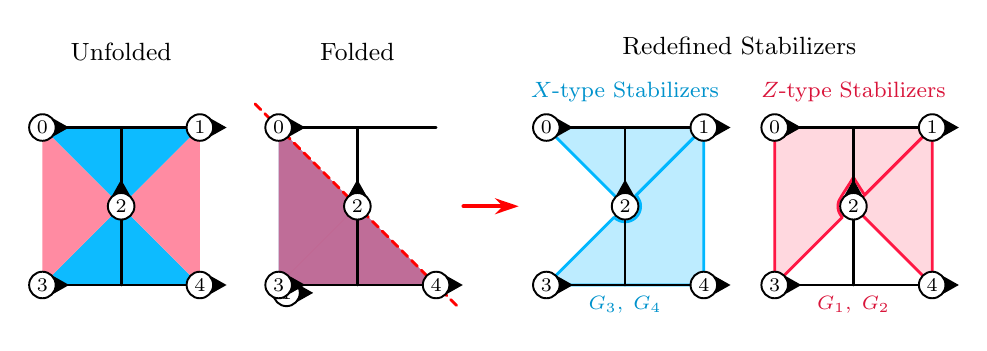
\begin{tikzpicture}[line cap=round,line join=round,thick,scale=1.0]
  \coordinate (Left)   at (-4.85, 0);
  \coordinate (Middle) at (-1.85, 0);
  \coordinate (XGrid)  at ( 1.55, 0);
  \coordinate (ZGrid)  at ( 4.45, 0);

  \node[above,font=\small] at ($(Left)+(0,1.72)$) {Unfolded};
  \node[above,font=\small] at ($(Middle)+(0,1.72)$) {Folded};
  \node[above,font=\small] at ($(XGrid)!0.5!(ZGrid)+(0,1.80)$) {Redefined Stabilizers};
  \node[above,font=\footnotesize,text=Xcol!80!black] at ($(XGrid)+(0,1.20)$) {$X$-type Stabilizers};
  \node[above,font=\footnotesize,text=Zcol!85!black] at ($(ZGrid)+(0,1.20)$) {$Z$-type Stabilizers};
  \node[font=\scriptsize,text=Xcol!80!black] at ($(XGrid)+(0,-1.25)$) {$G_3,\;G_4$};
  \node[font=\scriptsize,text=Zcol!85!black] at ($(ZGrid)+(0,-1.25)$) {$G_1,\;G_2$};

  % --- Left Patch (Unfolded) ---
  \begin{scope}[shift={(Left)}]
    \FiveQPatchFilled
    \FiveQPatchCircles
  \end{scope}

  % --- Middle Patch (Folded) ---
  \begin{scope}[shift={(Middle)}]
    \FiveQPatchOverlapped
    \def\m{0.30}
    \draw[dashed, draw=red, line width=1pt, dash pattern=on 3pt off 2pt]
      ($(q0)+(-\m,\m)$) -- ($(q4)+(\m,-\m)$);
    \FiveQPatchCirclesOneUnderThree
  \end{scope}

  \draw[-{Stealth[length=3mm,width=2mm]},red,line width=1.6pt]
    ($(Middle)+(1.35,0)$) -- ($(XGrid)+(-1.35,0)$);

  % --- Redefined X-type grid ---
  \begin{scope}[shift={(XGrid)}]
    \FiveQPatchRedefinedXGrid
    \FiveQPatchCircles
  \end{scope}

  % --- Redefined Z-type grid ---
  \begin{scope}[shift={(ZGrid)}]
    \FiveQPatchRedefinedZGrid
    \FiveQPatchCircles
  \end{scope}
\end{tikzpicture}
\caption{5-Qutrit Surface Code Patch}
\end{subfigure}

\vspace{2.0ex}

% ===================== (b) Definition =====================
\hspace*{-1.5em}
\begin{subfigure}[c]{0.48\textwidth}
\centering
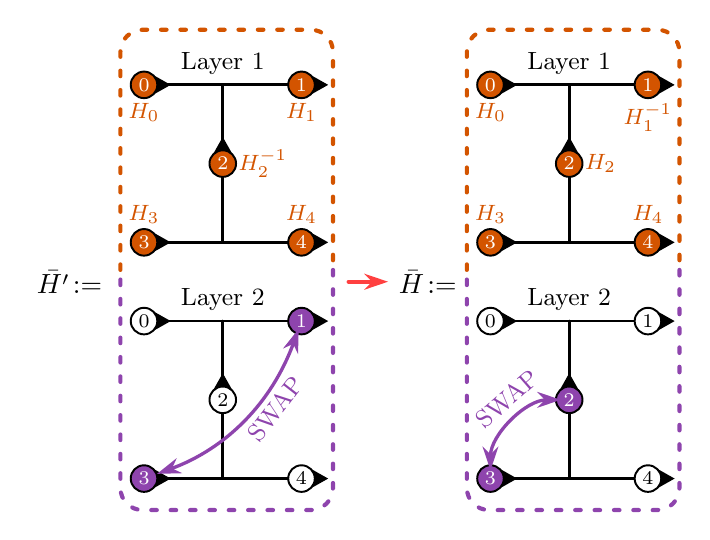
\begin{tikzpicture}[line cap=round,line join=round,thick,scale=1.0]
  \coordinate (LeftTop) at (-2.2,  1.50);
  \coordinate (LeftBot) at (-2.2, -1.50);
  \coordinate (RightTop) at ( 2.2,  1.50);
  \coordinate (RightBot) at ( 2.2, -1.50);

  \node[scale=1.0, anchor=east] at ($(LeftTop)+(-1.4, -1.5)$) {$\bar{H'}\!:=$};
  \node[scale=1.0, anchor=east] (HLabel) at ($(RightTop)+(-1.3, -1.5)$) {$\bar{H}\!:=$};

  \def\lw{1.5pt} \def\rc{8pt}
  % LEFT BOX 
  \path let \p1 = ($(LeftTop)+(-1.3,1.7)$), \p2 = ($(LeftBot)+(1.4,-1.4)$)
        in coordinate (LTL) at (\x1,\y1) coordinate (LBR) at (\x2,\y2)
           coordinate (LTR) at (\x2,\y1) coordinate (LBL) at (\x1,\y2);
  \coordinate (LMidLeft) at ($(LTL)!0.5!(LBL)$); \coordinate (LMidRight) at ($(LTR)!0.5!(LBR)$);
  \draw[HCol, dash pattern=on 2pt off 5pt, line width=\lw, rounded corners=\rc] (LMidLeft)--(LTL)--(LTR)--(LMidRight);
  \draw[SwapCol, dash pattern=on 2pt off 5pt, line width=\lw, rounded corners=\rc] (LMidRight)--(LBR)--(LBL)--(LMidLeft);

  % RIGHT BOX
  \path let \p1 = ($(RightTop)+(-1.3,1.7)$), \p2 = ($(RightBot)+(1.4,-1.4)$)
        in coordinate (RTL) at (\x1,\y1) coordinate (RBR) at (\x2,\y2)
           coordinate (RTR) at (\x2,\y1) coordinate (RBL) at (\x1,\y2);
  \coordinate (RMidLeft) at ($(RTL)!0.5!(RBL)$); \coordinate (RMidRight) at ($(RTR)!0.5!(RBR)$);
  \draw[HCol, dash pattern=on 2pt off 5pt, line width=\lw, rounded corners=\rc] (RMidLeft)--(RTL)--(RTR)--(RMidRight);
  \draw[SwapCol, dash pattern=on 2pt off 5pt, line width=\lw, rounded corners=\rc] (RMidRight)--(RBR)--(RBL)--(RMidLeft);

  \begin{scope}[shift={(LeftTop)}]
    \FiveQPatchEdges
    \foreach \P/\txt in {q0/0,q1/1,q2/2,q3/3,q4/4}{ \draw[line width=\qdLine,fill=HCol] (\P) circle (\qdR); \node[font=\numFont, text=white] at (\P) {\txt}; }
    \WedgeArrow{q0}{0}\WedgeArrow{q1}{0}\WedgeArrow{q3}{0}\WedgeArrow{q4}{0}\WedgeArrow{q2}{90}
    \node[anchor=south, font=\small, yshift=0mm] at (0, 1.0) {Layer 1};
    \begin{scope}[text=HCol, font=\footnotesize]
       \node[below, yshift=-3pt] at (q0) {$H_0$}; \node[below, yshift=-3pt] at (q1) {$H_1$};
       \node[right, xshift=2pt]  at (q2) {$H_2^{-1}$}; \node[above, yshift=3pt]  at (q3) {$H_3$}; \node[above, yshift=3pt]  at (q4) {$H_4$};
    \end{scope}
  \end{scope}

  \begin{scope}[shift={(LeftBot)}]
    \FiveQPatchEdges
    \foreach \P/\txt in {q0/0,q2/2,q4/4}{ \draw[line width=\qdLine,fill=white] (\P) circle (\qdR); \node[font=\numFont] at (\P) {\txt}; }
    \foreach \P/\txt in {q1/1,q3/3}{ \draw[line width=\qdLine,fill=SwapCol] (\P) circle (\qdR); \node[font=\numFont, text=white] at (\P) {\txt}; }
    \WedgeArrow{q0}{0}\WedgeArrow{q1}{0}\WedgeArrow{q3}{0}\WedgeArrow{q4}{0}\WedgeArrow{q2}{90}
    \node[anchor=south, font=\small, yshift=0mm] at (0, 1.0) {Layer 2};
    \draw[{Stealth[length=3mm,width=2mm]}-{Stealth[length=3mm,width=2mm]}, color=SwapCol, line width=1.2pt, shorten >=5pt, shorten <=3pt]
      (q1) to[bend left=25] node[midway, below right, rotate=52, xshift=-7pt, font=\small] {SWAP} (q3);
  \end{scope}

  \draw[-{Stealth[length=3mm,width=2mm]},red!75,line width=1.6pt] (-0.6, 0) -- (-0.1, 0);

  \begin{scope}[shift={(RightTop)}]
    \FiveQPatchEdges
    \foreach \P/\txt in {q0/0,q1/1,q2/2,q3/3,q4/4}{ \draw[line width=\qdLine,fill=HCol] (\P) circle (\qdR); \node[font=\numFont, text=white] at (\P) {\txt}; }
    \WedgeArrow{q0}{0}\WedgeArrow{q1}{0}\WedgeArrow{q3}{0}\WedgeArrow{q4}{0}\WedgeArrow{q2}{90}
    \node[anchor=south, font=\small, yshift=0mm] at (0, 1.0) {Layer 1};
    \begin{scope}[text=HCol, font=\footnotesize]
       \node[below, yshift=-3pt] at (q0) {$H_0$}; \node[below, yshift=-3pt] at (q1) {$H_1^{-1}$};
       \node[right, xshift=2pt]  at (q2) {$H_2$}; \node[above, yshift=3pt]  at (q3) {$H_3$}; \node[above, yshift=3pt]  at (q4) {$H_4$};
    \end{scope}
  \end{scope}

  \begin{scope}[shift={(RightBot)}]
    \FiveQPatchEdges
    \foreach \P/\txt in {q0/0,q1/1,q4/4}{ \draw[line width=\qdLine,fill=white] (\P) circle (\qdR); \node[font=\numFont] at (\P) {\txt}; }
    \foreach \P/\txt in {q2/2,q3/3}{ \draw[line width=\qdLine,fill=SwapCol] (\P) circle (\qdR); \node[font=\numFont, text=white] at (\P) {\txt}; }
    \WedgeArrow{q0}{0}\WedgeArrow{q1}{0}\WedgeArrow{q3}{0}\WedgeArrow{q4}{0}\WedgeArrow{q2}{90}
    \node[anchor=south, font=\small, yshift=0mm] at (0, 1.0) {Layer 2};
    \draw[{Stealth[length=3mm,width=2mm]}-{Stealth[length=3mm,width=2mm]}, color=SwapCol, line width=1.2pt, shorten >=3pt, shorten <=3pt]
      (q2) to[bend right=45] node[midway, below, xshift =-7pt, yshift=14pt, rotate=41, font=\small] {SWAP} (q3);
  \end{scope}
\end{tikzpicture}
\caption{Logical $H$}
\label{fig: logical H}
\end{subfigure}
\quad
% ===================== (c) S Definition =====================
\begin{subfigure}[c]{0.48\textwidth}
\centering
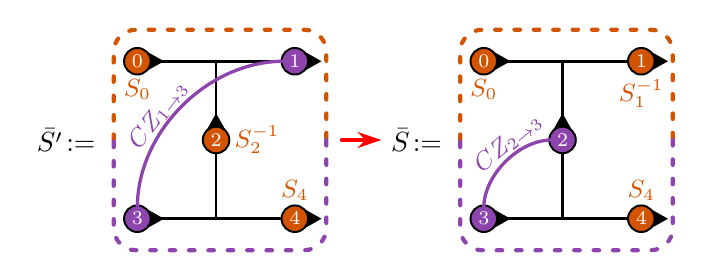
\begin{tikzpicture}[line cap=round,line join=round,thick,scale=1.0]
  \coordinate (Left)  at (-2.2, 0);
  \coordinate (Right) at ( 2.2, 0);
  \def\lw{1.5pt} \def\rc{8pt}

  \coordinate (LTL) at ($(Left)+(-1.3, 1.4)$); \coordinate (LBR) at ($(Left)+(1.4, -1.4)$);
  \coordinate (LTR) at ($(Left)+(1.4, 1.4)$);  \coordinate (LBL) at ($(Left)+(-1.3, -1.4)$);
  \coordinate (LMidLeft) at ($(LTL)!0.5!(LBL)$); \coordinate (LMidRight) at ($(LTR)!0.5!(LBR)$);
  \draw[HCol, dash pattern=on 2pt off 5pt, line width=\lw, rounded corners=\rc] (LMidLeft)--(LTL)--(LTR)--(LMidRight);
  \draw[SwapCol, dash pattern=on 2pt off 5pt, line width=\lw, rounded corners=\rc] (LMidRight)--(LBR)--(LBL)--(LMidLeft);

  \coordinate (RTL) at ($(Right)+(-1.3, 1.4)$); \coordinate (RBR) at ($(Right)+(1.4, -1.4)$);
  \coordinate (RTR) at ($(Right)+(1.4, 1.4)$);  \coordinate (RBL) at ($(Right)+(-1.3, -1.4)$);
  \coordinate (RMidLeft) at ($(RTL)!0.5!(RBL)$); \coordinate (RMidRight) at ($(RTR)!0.5!(RBR)$);
  \draw[HCol, dash pattern=on 2pt off 5pt, line width=\lw, rounded corners=\rc] (RMidLeft)--(RTL)--(RTR)--(RMidRight);
  \draw[SwapCol, dash pattern=on 2pt off 5pt, line width=\lw, rounded corners=\rc] (RMidRight)--(RBR)--(RBL)--(RMidLeft);

  \node[scale=1.0, anchor=east] at ($(Left)+(-1.4, 0)$) {$\bar{S'}\!:=$};
  \node[scale=1.0, anchor=east] (SLabel) at ($(Right)+(-1.4, 0)$) {$\bar{S}\!:=$};

  \newcommand{\DrawLHSPattern}{
      \FiveQPatchEdges
      \foreach \P in {q0, q2, q4} { \draw[line width=\qdLine,fill=HCol] (\P) circle (\qdR); }
      \foreach \P in {q1, q3} { \draw[line width=\qdLine,fill=SwapCol] (\P) circle (\qdR); }
      \foreach \P/\txt in {q0/0,q1/1,q2/2,q3/3,q4/4}{ \node[font=\numFont, text=white] at (\P) {\txt}; }
      \WedgeArrow{q0}{0}\WedgeArrow{q1}{0}\WedgeArrow{q3}{0}\WedgeArrow{q4}{0}\WedgeArrow{q2}{90}
      \node[text=HCol, font=\small, below, yshift=-3pt] at (q0) {$S_0$};
      \node[text=HCol, font=\small, right, xshift=3pt] at (q2) {$S_2^{-1}$};
      \node[text=HCol, font=\small, above, yshift=3pt] at (q4) {$S_4$};
      \draw[color=SwapCol, line width=1.2pt, shorten <=4pt, shorten >=4pt] 
         (q1) to[out=180, in=90] coordinate[pos=0.45] (mid) (q3);
      \node[text=SwapCol, font=\small, rotate=52, anchor=south, xshift=-12pt, yshift=-1pt] at (mid) {$CZ_{1\to 3}$};
  }
  \newcommand{\DrawRHSPattern}{
      \FiveQPatchEdges
      \foreach \P in {q0, q1, q4} { \draw[line width=\qdLine,fill=HCol] (\P) circle (\qdR); }
      \foreach \P in {q2, q3} { \draw[line width=\qdLine,fill=SwapCol] (\P) circle (\qdR); }
      \foreach \P/\txt in {q0/0,q1/1,q2/2,q3/3,q4/4}{ \node[font=\numFont, text=white] at (\P) {\txt}; }
      \WedgeArrow{q0}{0}\WedgeArrow{q1}{0}\WedgeArrow{q3}{0}\WedgeArrow{q4}{0}\WedgeArrow{q2}{90}
      \node[text=HCol, font=\small, below, yshift=-3pt] at (q0) {$S_0$};
      \node[text=HCol, font=\small, below, yshift=-3pt] at (q1) {$S_1^{-1}$};
      \node[text=HCol, font=\small, above, yshift=3pt] at (q4) {$S_4$};
      \draw[color=SwapCol, line width=1.2pt, shorten <=4pt, shorten >=4pt] 
         (q3) to[out=90, in=180] coordinate[pos=0.5] (midR) (q2);
      \node[text=SwapCol, font=\small, rotate=40, anchor=south, xshift=5pt, yshift=-2pt] at (midR) {$CZ_{2\to 3}$};
  }
  \begin{scope}[shift={(Left)}] \DrawLHSPattern \end{scope}
  \begin{scope}[shift={(Right)}] \DrawRHSPattern \end{scope}
  \draw[-{Stealth[length=3mm,width=2mm]},red,line width=1.6pt] (-0.6, 0) -- (-0.1, 0);
\end{tikzpicture}
\caption{Logical $S$}
\label{fig: logical S}
\end{subfigure}

\vspace{2.0ex}

% ===================== (d) Parallel Operations =====================
\begin{subfigure}[b]{0.9\textwidth}
\centering
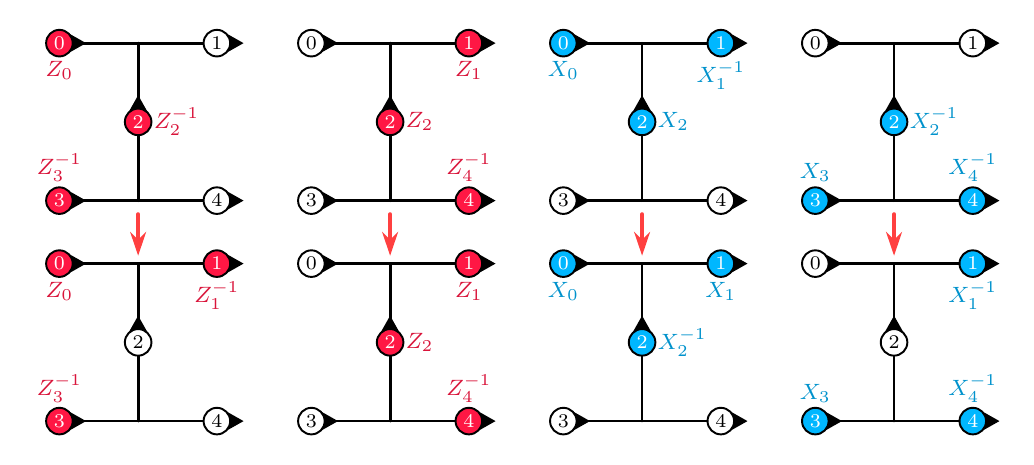
\begin{tikzpicture}[line cap=round,line join=round,thick,scale=1.0]
  \def\yTop{1.6} \def\yBot{-1.2}

  % COL 1
  \def\x{-4.8}
  \begin{scope}[shift={(\x, \yTop)}]
     \FiveQPatchEdges
     \foreach \P/\txt in {q1/1, q4/4}{ \draw[line width=\qdLine,fill=white] (\P) circle (\qdR); \node[font=\numFont] at (\P) {\txt}; }
     \foreach \P/\txt in {q0/0, q2/2, q3/3}{ \draw[line width=\qdLine,fill=Zcol] (\P) circle (\qdR); \node[font=\numFont, text=white] at (\P) {\txt}; }
     \WedgeArrow{q0}{0}\WedgeArrow{q1}{0}\WedgeArrow{q3}{0}\WedgeArrow{q4}{0}\WedgeArrow{q2}{90}
     \begin{scope}[text=Zcol!85!black, font=\footnotesize]
        \node[below, yshift=-3pt] at (q0) {$Z_0$}; \node[right, xshift=2pt] at (q2) {$Z_2^{-1}$}; \node[above, yshift=3pt] at (q3) {$Z_3^{-1}$};
     \end{scope}
  \end{scope}
  \begin{scope}[shift={(\x, \yBot)}]
     \FiveQPatchEdges
     \foreach \P/\txt in {q2/2, q4/4}{ \draw[line width=\qdLine,fill=white] (\P) circle (\qdR); \node[font=\numFont] at (\P) {\txt}; }
     \foreach \P/\txt in {q0/0, q1/1, q3/3}{ \draw[line width=\qdLine,fill=Zcol] (\P) circle (\qdR); \node[font=\numFont, text=white] at (\P) {\txt}; }
     \WedgeArrow{q0}{0}\WedgeArrow{q1}{0}\WedgeArrow{q3}{0}\WedgeArrow{q4}{0}\WedgeArrow{q2}{90}
     \begin{scope}[text=Zcol!85!black, font=\footnotesize]
        \node[below, yshift=-3pt] at (q0) {$Z_0$}; \node[below, yshift=-3pt] at (q1) {$Z_1^{-1}$}; \node[above, yshift=3pt] at (q3) {$Z_3^{-1}$};
     \end{scope}
  \end{scope}
  \draw[-{Stealth[length=3mm,width=2mm]},red!75,line width=1.6pt] (\x, 0.425) -- (\x, -0.1);

  % COL 2
  \def\x{-1.6}
  \begin{scope}[shift={(\x, \yTop)}]
     \FiveQPatchEdges
     \foreach \P/\txt in {q0/0, q3/3}{ \draw[line width=\qdLine,fill=white] (\P) circle (\qdR); \node[font=\numFont] at (\P) {\txt}; }
     \foreach \P/\txt in {q1/1, q2/2, q4/4}{ \draw[line width=\qdLine,fill=Zcol] (\P) circle (\qdR); \node[font=\numFont, text=white] at (\P) {\txt}; }
     \WedgeArrow{q0}{0}\WedgeArrow{q1}{0}\WedgeArrow{q3}{0}\WedgeArrow{q4}{0}\WedgeArrow{q2}{90}
     \begin{scope}[text=Zcol!85!black, font=\footnotesize]
        \node[below, yshift=-3pt] at (q1) {$Z_1$}; \node[right, xshift=2pt] at (q2) {$Z_2$}; \node[above, yshift=3pt] at (q4) {$Z_4^{-1}$};
     \end{scope}
  \end{scope}
  \begin{scope}[shift={(\x, \yBot)}]
     \FiveQPatchEdges
     \foreach \P/\txt in {q0/0, q3/3}{ \draw[line width=\qdLine,fill=white] (\P) circle (\qdR); \node[font=\numFont] at (\P) {\txt}; }
     \foreach \P/\txt in {q1/1, q2/2, q4/4}{ \draw[line width=\qdLine,fill=Zcol] (\P) circle (\qdR); \node[font=\numFont, text=white] at (\P) {\txt}; }
     \WedgeArrow{q0}{0}\WedgeArrow{q1}{0}\WedgeArrow{q3}{0}\WedgeArrow{q4}{0}\WedgeArrow{q2}{90}
     \begin{scope}[text=Zcol!85!black, font=\footnotesize]
        \node[below, yshift=-3pt] at (q1) {$Z_1$}; \node[right, xshift=2pt] at (q2) {$Z_2$}; \node[above, yshift=3pt] at (q4) {$Z_4^{-1}$};
     \end{scope}
  \end{scope}
  \draw[-{Stealth[length=3mm,width=2mm]},red!75,line width=1.6pt] (\x, 0.425) -- (\x, -0.1);

  % COL 3
  \def\x{1.6}
  \begin{scope}[shift={(\x, \yTop)}]
     \FiveQPatchEdges
     \foreach \P/\txt in {q3/3, q4/4}{ \draw[line width=\qdLine,fill=white] (\P) circle (\qdR); \node[font=\numFont] at (\P) {\txt}; }
     \foreach \P/\txt in {q0/0, q1/1, q2/2}{ \draw[line width=\qdLine,fill=Xcol] (\P) circle (\qdR); \node[font=\numFont, text=white] at (\P) {\txt}; }
     \WedgeArrow{q0}{0}\WedgeArrow{q1}{0}\WedgeArrow{q3}{0}\WedgeArrow{q4}{0}\WedgeArrow{q2}{90}
     \begin{scope}[text=Xcol!80!black, font=\footnotesize]
        \node[below, yshift=-3pt] at (q0) {$X_0$}; \node[below, yshift=-3pt] at (q1) {$X_1^{-1}$}; \node[right, xshift=2pt] at (q2) {$X_2$};
     \end{scope}
  \end{scope}
  \begin{scope}[shift={(\x, \yBot)}]
     \FiveQPatchEdges
     \foreach \P/\txt in {q3/3, q4/4}{ \draw[line width=\qdLine,fill=white] (\P) circle (\qdR); \node[font=\numFont] at (\P) {\txt}; }
     \foreach \P/\txt in {q0/0, q1/1, q2/2}{ \draw[line width=\qdLine,fill=Xcol] (\P) circle (\qdR); \node[font=\numFont, text=white] at (\P) {\txt}; }
     \WedgeArrow{q0}{0}\WedgeArrow{q1}{0}\WedgeArrow{q3}{0}\WedgeArrow{q4}{0}\WedgeArrow{q2}{90}
     \begin{scope}[text=Xcol!80!black, font=\footnotesize]
        \node[below, yshift=-3pt] at (q0) {$X_0$}; \node[below, yshift=-3pt] at (q1) {$X_1$}; \node[right, xshift=2pt] at (q2) {$X_2^{-1}$};
     \end{scope}
  \end{scope}
  \draw[-{Stealth[length=3mm,width=2mm]},red!75,line width=1.6pt] (\x, 0.425) -- (\x, -0.1);

  % COL 4
  \def\x{4.8}
  \begin{scope}[shift={(\x, \yTop)}]
     \FiveQPatchEdges
     \foreach \P/\txt in {q0/0, q1/1}{ \draw[line width=\qdLine,fill=white] (\P) circle (\qdR); \node[font=\numFont] at (\P) {\txt}; }
     \foreach \P/\txt in {q2/2, q3/3, q4/4}{ \draw[line width=\qdLine,fill=Xcol] (\P) circle (\qdR); \node[font=\numFont, text=white] at (\P) {\txt}; }
     \WedgeArrow{q0}{0}\WedgeArrow{q1}{0}\WedgeArrow{q3}{0}\WedgeArrow{q4}{0}\WedgeArrow{q2}{90}
     \begin{scope}[text=Xcol!80!black, font=\footnotesize]
        \node[right, xshift=2pt] at (q2) {$X_2^{-1}$}; \node[above, yshift=3pt] at (q3) {$X_3$}; \node[above, yshift=3pt] at (q4) {$X_4^{-1}$};
     \end{scope}
  \end{scope}
  \begin{scope}[shift={(\x, \yBot)}]
     \FiveQPatchEdges
     \foreach \P/\txt in {q0/0, q2/2}{ \draw[line width=\qdLine,fill=white] (\P) circle (\qdR); \node[font=\numFont] at (\P) {\txt}; }
     \foreach \P/\txt in {q1/1, q3/3, q4/4}{ \draw[line width=\qdLine,fill=Xcol] (\P) circle (\qdR); \node[font=\numFont, text=white] at (\P) {\txt}; }
     \WedgeArrow{q0}{0}\WedgeArrow{q1}{0}\WedgeArrow{q3}{0}\WedgeArrow{q4}{0}\WedgeArrow{q2}{90}
     \begin{scope}[text=Xcol!80!black, font=\footnotesize]
        \node[below, yshift=-3pt] at (q1) {$X_1^{-1}$}; \node[above, yshift=3pt] at (q3) {$X_3$}; \node[above, yshift=3pt] at (q4) {$X_4^{-1}$};
     \end{scope}
  \end{scope}
  \draw[-{Stealth[length=3mm,width=2mm]},red!75,line width=1.6pt] (\x, 0.425) -- (\x, -0.1);
\end{tikzpicture}
\caption{Stabilizers for the $[[5,1,2]]_3$ code}
\end{subfigure}

\vspace{2.0ex}
% ===================== (e) Logical X =====================
\begin{subfigure}[c]{0.35\textwidth}
\centering
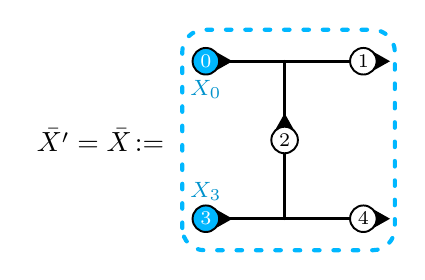
\begin{tikzpicture}[line cap=round,line join=round,thick,scale=1.0]
  \node[scale=1.0, anchor=east] at (-1.4, 0) {$\bar{X'}=\bar{X}\!:=$};
   
  % Added blue box
  \def\lw{1.5pt} \def\rc{8pt}
  \coordinate (LTL_X) at (-1.3, 1.4); \coordinate (LBR_X) at (1.4, -1.4);
  \coordinate (LTR_X) at ( 1.4, 1.4); \coordinate (LBL_X) at (-1.3, -1.4);
  \draw[Xcol, dash pattern=on 2pt off 5pt, line width=\lw, rounded corners=\rc] (LBL_X)--(LTL_X)--(LTR_X)--(LBR_X)--cycle;
   
  \FiveQPatchEdges
  \foreach \P/\txt in {q1/1, q2/2, q4/4}{ \draw[line width=\qdLine,fill=white] (\P) circle (\qdR); \node[font=\numFont] at (\P) {\txt}; }
  \foreach \P/\txt in {q0/0, q3/3}{ \draw[line width=\qdLine,fill=Xcol] (\P) circle (\qdR); \node[font=\numFont, text=white] at (\P) {\txt}; }
  \WedgeArrow{q0}{0}\WedgeArrow{q1}{0}\WedgeArrow{q3}{0}\WedgeArrow{q4}{0}\WedgeArrow{q2}{90}
  \begin{scope}[text=Xcol!80!black, font=\footnotesize]
     \node[below, yshift=-3pt] at (q0) {$X_0$};
     \node[above, yshift=3pt]  at (q3) {$X_3$};
  \end{scope}
\end{tikzpicture}
\caption{Logical $X$}
\end{subfigure}
\quad
% ===================== (f) Logical Z =====================
\begin{subfigure}[c]{0.6\textwidth}
\centering
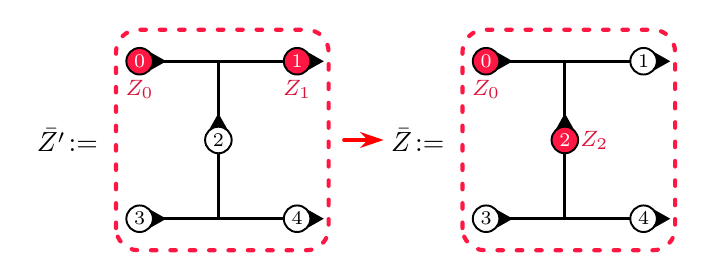
\begin{tikzpicture}[line cap=round,line join=round,thick,scale=1.0]
  % Define centers
  \coordinate (Left)  at (-2.2, 0);
  \coordinate (Right) at ( 2.2, 0);

  % Labels
  \node[scale=1.0, anchor=east] at ($(Left)+(-1.4, 0)$) {$\bar{Z'}\!:=$};
  \node[scale=1.0, anchor=east] at ($(Right)+(-1.4, 0)$) {$\bar{Z}\!:=$};
   
  % Added red boxes
  \def\lw{1.5pt} \def\rc{8pt}
  % Left Box
  \coordinate (LTL_Z) at ($(Left)+(-1.3, 1.4)$); \coordinate (LBR_Z) at ($(Left)+(1.4, -1.4)$);
  \coordinate (LTR_Z) at ($(Left)+(1.4, 1.4)$); \coordinate (LBL_Z) at ($(Left)+(-1.3, -1.4)$);
  \draw[Zcol, dash pattern=on 2pt off 5pt, line width=\lw, rounded corners=\rc] (LBL_Z)--(LTL_Z)--(LTR_Z)--(LBR_Z)--cycle;

  % Right Box
  \coordinate (RTL_Z) at ($(Right)+(-1.3, 1.4)$); \coordinate (RBR_Z) at ($(Right)+(1.4, -1.4)$);
  \coordinate (RTR_Z) at ($(Right)+(1.4, 1.4)$); \coordinate (RBL_Z) at ($(Right)+(-1.3, -1.4)$);
  \draw[Zcol, dash pattern=on 2pt off 5pt, line width=\lw, rounded corners=\rc] (RBL_Z)--(RTL_Z)--(RTR_Z)--(RBR_Z)--cycle;

  % Left Patch: Z0 Z1
  \begin{scope}[shift={(Left)}]
     \FiveQPatchEdges
     \foreach \P/\txt in {q2/2, q3/3, q4/4}{ \draw[line width=\qdLine,fill=white] (\P) circle (\qdR); \node[font=\numFont] at (\P) {\txt}; }
     \foreach \P/\txt in {q0/0, q1/1}{ \draw[line width=\qdLine,fill=Zcol] (\P) circle (\qdR); \node[font=\numFont, text=white] at (\P) {\txt}; }
     \WedgeArrow{q0}{0}\WedgeArrow{q1}{0}\WedgeArrow{q3}{0}\WedgeArrow{q4}{0}\WedgeArrow{q2}{90}
     \begin{scope}[text=Zcol!85!black, font=\footnotesize]
        \node[below, yshift=-3pt] at (q0) {$Z_0$};
        \node[below, yshift=-3pt] at (q1) {$Z_1$};
     \end{scope}
  \end{scope}

  % Right Patch: Z0 Z2
  \begin{scope}[shift={(Right)}]
     \FiveQPatchEdges
     \foreach \P/\txt in {q1/1, q3/3, q4/4}{ \draw[line width=\qdLine,fill=white] (\P) circle (\qdR); \node[font=\numFont] at (\P) {\txt}; }
     \foreach \P/\txt in {q0/0, q2/2}{ \draw[line width=\qdLine,fill=Zcol] (\P) circle (\qdR); \node[font=\numFont, text=white] at (\P) {\txt}; }
     \WedgeArrow{q0}{0}\WedgeArrow{q1}{0}\WedgeArrow{q3}{0}\WedgeArrow{q4}{0}\WedgeArrow{q2}{90}
     \begin{scope}[text=Zcol!85!black, font=\footnotesize]
        \node[below, yshift=-3pt] at (q0) {$Z_0$};
        \node[right, xshift=2pt]  at (q2) {$Z_2$};
     \end{scope}
  \end{scope}

  % Arrow in middle (adjusted for gap)
  \draw[-{Stealth[length=3mm,width=2mm]},red,line width=1.6pt] (-0.6, 0) -- (-0.1, 0);

\end{tikzpicture}
\caption{Logical $Z$}
\end{subfigure}
% END OF PAGE 1
\end{figure}

\begin{figure}[H]\ContinuedFloat
\centering
% ===== MAIN CAPTION HERE =====
\caption{Comparison of 5-qutrit surface code definitions and logical operators. 
(a) The left-hand side (LHS) shows the conventional folded and unfolded definitions from \cite{Moussa2016}. Blue and red regions represent truncated conventional $X$- and $Z$-type stabilizers, respectively. In the folded version, blended colors indicate the mirror duality between these stabilizers. The right-hand side (RHS) illustrates the proposed convention, with the redefined $X$- and $Z$-type stabilizers shown on separate grids using colored patch perimeters. This avoids the folding procedure via local SWAPs, thereby eliminating the need for additional ancillas. 
(b) The proposed logical Hadamard gate, $\bar{H}$. Together with the logical Phase gate $\bar{S}$ shown in (c), these operators generate the single-qutrit logical Clifford group. Unlike the conventional $\bar{H'}$, this implementation requires only nearest-neighbor SWAP gates in Layer 2. 
(c) The proposed logical Phase gate, $\bar{S}$, which utilizes only nearest-neighbor $CZ$ gates, distinct from the conventional $\bar{S'}$. 
(d) Redefined $X$- and $Z$-type stabilizers, selected to be preserved by the logical Clifford group while maintaining mirror dual symmetry. 
(e) The logical $\bar{X}$ operator (unchanged). 
(f) The redefined logical $\bar{Z}$, constructed to commute with stabilizers and generate the Pauli group with $\bar{X}$, ensuring the Pauli group is preserved by the logical Clifford group.}
\label{fig: 5-qutrit-code}

\end{figure}



\subsubsection{Encoding Circuit}

To initialize the system in the code space, we employ a specific unitary circuit that maps the physical ground state $\ket{0}^{\otimes 5}$ to the logical state $\ket{\bar{+}}$. This state corresponds to the $+1$ eigenstate of the logical Pauli operator $\overline{X} = X_0 \otimes X_3$, defined in Eq.~\eqref{eq:logicalPauli}.

\begin{figure}[htbp]
    \centering
    \begin{quantikz}
      \lstick{$q_0: \ket{0}$} & \qw & \qw & \gate{X_3} & \gate{X_3} & \qw \\
      \lstick{$q_1: \ket{0}$} & \qw & \gate{X_3^{\dagger}} & \ctrl{-1} & \qw & \qw \\
      \lstick{$q_2: \ket{0}$} & \gate{H_3^{\dagger}} & \ctrl{-1} & \gate{X_3} & \qw & \qw \\
      \lstick{$q_3: \ket{0}$} & \gate{H_3^{\dagger}} & \qw & \qw & \ctrl{-3}  & \qw \\
      \lstick{$q_4: \ket{0}$} & \gate{H_3^{\dagger}} & \qw & \ctrl{-2}  & \qw  & \qw
    \end{quantikz}
    \caption{Non-fault-tolerant encoding circuit for the $[[5,1,2]]_3$ surface code. The circuit maps the physical state $\ket{0}^{\otimes 5}$ to the logical state $\ket{\bar{+}}$, which is the $+1$ eigenstate of the logical $\bar{X}$ operator. The gates denoted are qutrit Hadamard ($H_3$) and Generalized SUM/CNOT gates. Errors occurring during state preparation are accounted for as SPAM errors in the LRB protocol.}
    \label{fig:encoding_circuit}
\end{figure}

The encoding circuit shown in \autoref{fig:encoding_circuit} is a non-fault-tolerant state preparation sequence to minimize the use of ancillas and physical gate count. In the context of LRB, the quality of the encoding step is classified under State Preparation and Measurement (SPAM) errors. As established in standard RB theory, these SPAM errors are absorbed into the $A$ and $B$ parameters of the fidelity decay curve (Eq.~\eqref{eq:fseq}) and do not affect the extracted decay parameter $f$ or the estimated gate fidelity \cite{Magesan2011PRL,Magesan2012PRA}. Consequently, a compact, non-fault-tolerant encoding is sufficient for providing a consistent entry point into the logical code space for benchmarking purposes.


\subsection{Logical Randomized Benchmarking with Detection (LRB-D)}
\label{sub:lrb_d}

Standard Logical Randomized Benchmarking (LRB) characterizes the performance of a code by actively correcting errors using decoder feedback throughout the Clifford sequence \cite{Combes2017}. However, the $[[5,1,2]]_3$ code utilized in this work is a distance $d=2$ code. While it can detect the presence of any single-qutrit error, it cannot identify the specific error location and type without ambiguity. Consequently, the code violates the Knill-Laflamme error correction conditions for generic single-qutrit errors, making faithful error correction impossible.

To address this, we employ a detection-only variant of the protocol, denoted as LRB-D. Instead of attempting to correct errors and return the system to the code space, LRB-D treats the stabilizer measurements as a filter. We post-select exclusively on shots where the system remains in the code space. Thereby, discarding any experimental runs (shots) where a non-trivial error syndrome is detected. This effectively benchmarks the code's ability to preserve the logical information in the absence of detectable errors.

We initially simulate this protocol on the \texttt{sdim} qudit stabilizer simulator before executing it on hardware. This numerical validation allows us to verify the expected logical fidelity decay and the effectiveness of the post-selection filter under controlled noise models, establishing a necessary performance baseline prior to running the protocol on the IQM Garnet QPU.

\subsubsection{LRB-D Protocol}
The LRB-D protocol proceeds as follows, illustrated in \autoref{fig:lrb_d_full}:

\begin{enumerate}
    \item \textbf{Logical State Preparation:} Using the circuit in \autoref{fig:encoding_circuit}, the system is encoded into the logical state $\ket{\bar{+}}$, the $+1$ eigenstate of the logical $\bar{X}$ operator.
    
    \item \textbf{Random Logical Clifford Sequence:} A sequence of $m$ logical Clifford gates, $\mathcal{C} = \{\bar C_1, \bar C_2, \dots, \bar C_m\}$, sampled uniformly from the logical single-qutrit Clifford group, is applied to the encoded state.
    
    \textit{Simulation: To model the noisy experimental conditions, we insert the single-qudit noise channel of the chosen noise model (\autoref{sub:noise_models}) on the qudits involved in each logical operation. In the depolarizing model the channel is applied once to every involved qudit at the end of the decomposed logical gate, as illustrated in \autoref{fig:lrb_b}, while in the SI1000 model noise follows every physical gate at the rates of \autoref{tab:si1000-noise}.}
    
    \item \textbf{Inversion:} The sequence is inverted by applying $\bar C_{inv} = (\prod_{i=1}^m \bar C_i)^{-1}$. In the absence of logical errors, this returns the system to the $\ket{\bar{+}}$ state.
    
    \textit{Simulation: The inversion gate is treated identically to the random sequence, with the same local noise insertion applied to the relevant qudits immediately following the decomposed physical gates that make up the logical inverse.}
    
    \item \textbf{Stabilizer Measurement and Post-selection (Terminal and Intermediate Check):} 
    We measure the code stabilizers $G_1, \dots, G_4$ utilizing the syndrome extraction circuits depicted in \autoref{fig:lrb_c} and \autoref{fig:lrb_d}. This verification is implemented either as a single \emph{terminal check} immediately preceding the logical readout, or at \emph{arbitrary intervals} interspersed within the Clifford sequence $\{\bar C_1, \bar C_2, \dots, \bar C_m\}$. In the terminal-only case no ancilla circuits are run, and the check is instead evaluated classically from the terminal $X$-basis data readout, which determines the two $X$-type stabilizers alongside the logical measurement. The intermediate strategy utilizes continuous error detection by filtering the state trajectory, allowing only error-free shots to propagate to the subsequent gate. We strictly post-select on the trivial ``no-error'' syndrome across the checks performed:
    \begin{equation}
        \text{Keep shot if: } \forall k \in \{1, \dots, 4\}, \quad \text{outcome}(G_k) = 0 \pmod 3
    \end{equation}
    Any shot yielding a non-trivial syndrome (corresponding to eigenvalues $\omega$ or $\omega^2$, or integer outcomes 1 and 2) is discarded. This post-selection acts as a filter, excluding trajectories contaminated by detectable physical errors to isolate the logical gate fidelity.

    \textit{Simulation: In the numerical simulation of the syndrome extraction, we model interaction errors by inserting the two-qutrit channel $\mathcal{E}^{(2)}_{\mathcal{D}}$ of \autoref{sub:noise_models} immediately following every two-qudit gate (generalized $CX$ or $CX^\dagger$) interacting the ancilla and data qutrits. The single-qutrit channel is likewise applied to the ancilla immediately following the Hadamard gates ($H_3, H_3^{-1}$) in the $X$-type stabilizer circuits, as illustrated in \autoref{fig:lrb_d}. Under the SI1000 model the resets, readouts, and idling qutrits in these circuits carry the additional channels listed in \autoref{tab:si1000-noise}.}
    
    
    \item \textbf{Logical Measurement:} For the surviving shots, we execute the logical readout by measuring $q_0$ and $q_3$ in the $X$ basis as the logical operator is defined as $\bar{X} = X_0 \otimes X_3$. We obtain outcomes $m_0, m_3 \in \{0, 1, 2\}$. The logical measurement result $m_{\bar{X}}$ is determined by the modular sum of these physical outcomes:
    \begin{equation}
        m_{\bar{X}} = (m_0 + m_3) \pmod 3
    \end{equation}
    We then calculate the expectation value $\langle \bar{X} \rangle$ of the logical measurement, where the result $m_{\bar{X}}=0$ corresponds to the target eigenvalue $+1$:
    \begin{equation}
        \langle \bar{X} \rangle = P_0(1) + P_1(\omega) + P_2(\omega^2)
    \end{equation}
    Here, $P_j$ is the proportion of post-selected shots yielding the logical outcome $j$.
\end{enumerate}
\begin{figure}[H]
    \centering
    % --- Row 1: Parts (a) and (b) ---
    \begin{subfigure}[b]{0.63\textwidth}
        \centering
        \scalebox{0.72}{
        \begin{quantikz}
          \lstick{$\ket{0}$} & 
            \gate[wires=5]{\textcolor{LightBlue}{\ket{\bar{+}}\bra{\bar{+}}}} &
            \gate[wires=5]{\textcolor{red}{\bar C_1}} &
            \gate[wires=5]{\textcolor{purple}{\Lambda_{\mathcal{E}_{\mathcal{D}}}}} &
            \gate[wires=5]{\textcolor{red}{\bar C_2}} &
            \gate[wires=5]{\textcolor{purple}{\Lambda_{\mathcal{E}_{\mathcal{D}}}}} &
            \push{\dots} & \gate[wires=5]{\textcolor{red}{\bar C_m}} &
            \gate[wires=5]{\textcolor{purple}{\Lambda_{\mathcal{E}_{\mathcal{D}}}}} &
            \gate[wires=5]{\textcolor{red}{\bar C_{1:m}^{-1}}} &
            \gate[wires=5]{\textcolor{purple}{\Lambda_{\mathcal{E}_{\mathcal{D}}}}} &
            \meter{} &
            \qw \\
          \lstick{$\ket{0}$} & & & & & & \push{\dots} & & & & & \meter{} &\qw \\
          \lstick{$\ket{0}$} & & & & & & \push{\dots} & & & & & \meter{} &\qw \\
          \lstick{$\ket{0}$} & & & & & & \push{\dots} & & & & & \meter{} &\qw \\
          \lstick{$\ket{0}$} & & & & & & \push{\dots} & & & & & \meter{} &\qw \\
        \end{quantikz}
        }
        \vspace{-0.4cm}
        \caption{Simulated LRB-D circuit with local noise insertion}
        \label{fig:lrb_a}
    \end{subfigure}
    \hfill
    \begin{subfigure}[b]{0.35\textwidth}
    
        \centering
        \raisebox{0.8cm}{
        \scalebox{0.7}{
        \begin{quantikz}
          \lstick{$q_0: \ket{0}$} & \gate{S_3} & \gate{\textcolor{purple}{\mathcal{E}_{\mathcal{D}}}} & \qw \\
          \lstick{$q_1: \ket{0}$} & \gate{S_3^{-1}} & \gate{\textcolor{purple}{\mathcal{E}_{\mathcal{D}}}} & \qw \\
          \lstick{$q_2: \ket{0}$} & \ctrl{1} & \gate{\textcolor{purple}{\mathcal{E}_{\mathcal{D}}}} & \qw  \\
          \lstick{$q_3: \ket{0}$} & \gate{Z_3} & \gate{\textcolor{purple}{\mathcal{E}_{\mathcal{D}}}} & \qw \\  
          \lstick{$q_4: \ket{0}$} & \gate{S_3} & \gate{\textcolor{purple}{\mathcal{E}_{\mathcal{D}}}}& \qw
        \end{quantikz}
        }
        }
        \caption{$\mathcal{E}_{\mathcal{D}}$ on qutrits involved \newline in $\bar C_i$}
        \vspace{-0.4cm}
        \label{fig:lrb_b}
    \end{subfigure}
    \hspace{-1.0cm}
    \vspace{0.2cm}

    % --- Row 2: Parts (c) and (d) ---
    % Note: No \centering here inside the row logic, effectively.
    % The trailing \hfill at the very end of the row pushes these two to the left.
    
    % Part (c): Z-type Stabilizers
    \hspace{-2.6cm}
    \begin{subfigure}[b]{0.45\textwidth} % Reduced width slightly to ensure fit
        \centering
        % G1
       
        \scalebox{0.58}{
        \begin{quantikz}
          \lstick{$q_0$} & \ctrl{5} & \gate[wires=6]{\textcolor{purple}{\mathcal{E}^{(2)}_{\mathcal{D}}}} & \qw & \qw & \qw & \qw & \qw & \qw \\
          \lstick{$q_1$} & \qw & \qw & \ctrl{4} & \gate[wires=5]{\textcolor{purple}{\mathcal{E}^{(2)}_{\mathcal{D}}}} & \qw & \qw & \qw & \qw \\
          \lstick{$q_2$} & \qw & \qw & \qw & \qw & \qw & \qw & \qw & \qw \\
          \lstick{$q_3$} & \qw & \qw & \qw & \qw & \ctrl{2} & \gate[wires=3]{\textcolor{purple}{\mathcal{E}^{(2)}_{\mathcal{D}}}} & \qw & \qw \\  
          \lstick{$q_4$} & \qw & \qw & \qw & \qw & \qw & \qw & \qw & \qw \\
          \lstick{$a: \ket{0}$} & \gate{X_3} & \qw & \gate{X_3^{\dagger}} & \qw & \gate{X_3^{\dagger}} & \qw & \meter{} & \qw
        \end{quantikz}
        }
        \par \vspace{0.4cm}
        % G2
        \scalebox{0.58}{
        \begin{quantikz}
          \lstick{$q_0$} & \qw & \qw & \qw & \qw & \qw & \qw & \qw & \qw \\
          \lstick{$q_1$} & \ctrl{4} & \gate[wires=5]{\textcolor{purple}{\mathcal{E}^{(2)}_{\mathcal{D}}}} & \qw & \qw & \qw & \qw & \qw & \qw \\
          \lstick{$q_2$} & \qw & \qw & \ctrl{3} & \gate[wires=4]{\textcolor{purple}{\mathcal{E}^{(2)}_{\mathcal{D}}}} & \qw & \qw & \qw & \qw \\
          \lstick{$q_3$} & \qw & \qw & \qw & \qw & \qw & \qw & \qw & \qw  \\  
          \lstick{$q_4$} & \qw & \qw & \qw & \qw & \ctrl{1} & \gate[wires=2]{\textcolor{purple}{\mathcal{E}^{(2)}_{\mathcal{D}}}} & \qw & \qw \\
          \lstick{$a: \ket{0}$} & \gate{X_3} & \qw & \gate{X_3} & \qw & \gate{X_3^{\dagger}} & \qw & \meter{} & \qw
        \end{quantikz}
        }
        \captionsetup{margin={0.4cm, 0.4cm}}
        \caption{Syndrome extraction circuits for $Z$-type stabilizers: $Z_0Z_1^{-1}Z_3^{-1}$ and $Z_1Z_2Z_4^{-1}$}
        
        \label{fig:lrb_c}
    \end{subfigure}
    \hspace{-.5cm} % Small fixed gap between c and d
    % Part (d): X-type Stabilizers
    \begin{subfigure}[b]{0.45\textwidth}
        \centering
        % G3
        \scalebox{0.58}{
        \begin{quantikz}
          \lstick{$q_0$} & \qw & \qw & \gate{X_3} & \gate[wires=6]{\textcolor{purple}{\mathcal{E}^{(2)}_{\mathcal{D}}}} & \qw & \qw & \qw & \qw & \qw & \qw & \qw & \qw \\ % Added extra & \qw
          \lstick{$q_1$} & \qw & \qw & \qw & \qw & \gate{X_3} & \gate[wires=5]{\textcolor{purple}{\mathcal{E}^{(2)}_{\mathcal{D}}}} & \qw & \qw & \qw & \qw & \qw & \qw \\ % Added extra & \qw
          \lstick{$q_2$} & \qw & \qw & \qw & \qw & \qw & \qw & \gate{X_3^{\dagger}} & \gate[wires=4]{\textcolor{purple}{\mathcal{E}^{(2)}_{\mathcal{D}}}} & \qw & \qw & \qw & \qw \\ % Added extra & \qw
          \lstick{$q_3$} & \qw & \qw & \qw & \qw & \qw & \qw & \qw & \qw & \qw & \qw & \qw & \qw \\ % Added extra & \qw 
          \lstick{$q_4$} & \qw & \qw & \qw & \qw & \qw & \qw & \qw & \qw & \qw & \qw & \qw & \qw \\ % Added extra & \qw
          \lstick{$a: \ket{0}$} & \gate{H_3} & \gate{\textcolor{purple}{\mathcal{E}_{\mathcal{D}}}} & \ctrl{-5} & \qw & \ctrl{-4} & \qw & \ctrl{-3} & \qw & \gate{H_3^{-1}} & \gate{\textcolor{purple}{\mathcal{E}_{\mathcal{D}}}} & \meter{} & \qw
        \end{quantikz}
        }
        \par \vspace{0.4cm}
        % G4
        \scalebox{0.58}{
        \begin{quantikz}
          \lstick{$q_0$} & \qw & \qw & \qw & \qw & \qw & \qw & \qw & \qw & \qw & \qw & \qw & \qw \\ % Added extra & \qw
          \lstick{$q_1$} & \qw & \qw & \gate{X_3^{\dagger}} & \gate[wires=5]{\textcolor{purple}{\mathcal{E}^{(2)}_{\mathcal{D}}}} & \qw & \qw & \qw & \qw & \qw & \qw & \qw & \qw \\ % Added extra & \qw
          \lstick{$q_2$} & \qw & \qw & \qw & \qw & \qw & \qw & \qw & \qw & \qw & \qw & \qw & \qw \\ % Added extra & \qw
          \lstick{$q_3$} & \qw & \qw & \qw & \qw & \gate{X_3} & \gate[wires=3]{\textcolor{purple}{\mathcal{E}^{(2)}_{\mathcal{D}}}} & \qw & \qw & \qw & \qw & \qw & \qw \\ % Added extra & \qw 
          \lstick{$q_4$} & \qw & \qw & \qw & \qw & \qw & \qw & \gate{X_3^{\dagger}} & \gate[wires=2]{\textcolor{purple}{\mathcal{E}^{(2)}_{\mathcal{D}}}} & \qw & \qw & \qw  & \qw \\ % Added extra & \qw
          \lstick{$a: \ket{0}$} & \gate{H_3} & \gate{\textcolor{purple}{\mathcal{E}_{\mathcal{D}}}} & \ctrl{-4} & \qw & \ctrl{-2} & \qw & \ctrl{-1} & \qw & \gate{H_3^{-1}} & \gate{\textcolor{purple}{\mathcal{E}_{\mathcal{D}}}} & \meter{} & \qw
        \end{quantikz}
        }
        \captionsetup{margin={1cm, -1.2cm}}
        \caption{Syndrome extraction circuits for $X$-type stabilizers: $X_0X_1X_2^{-1}$ and $X_1^{-1}X_3X_4^{-1}$}
        \label{fig:lrb_d}
    \end{subfigure}
    \hfill % <--- This pushes (c) and (d) to the left

    \caption{Overview of the simulated LRB-D protocol. (a) The full protocol circuit illustrating the $\ket{\bar +}$ initialization, the random logical Clifford sequence, inversion, and measurement, with effective single qutrit depolarizing noise $\Lambda_{\mathcal{E}_{\mathcal{D}}}$ inserted after each gate. (b) A detailed view of the physical simulation model, where single-qutrit depolarizing errors $\mathcal{E}_{\mathcal{D}}$ are applied after every physical gate in a decomposition. (c) Syndrome extraction circuits for Z-type stabilizers, incorporating two-qutrit depolarizing noise $\mathcal{E}^{(2)}_{\mathcal{D}}$ after entangling gates. (d) Syndrome extraction circuits for X-type stabilizers, featuring additional single-qutrit noise on the ancilla. These circuits enable post-selection at either the terminal step or intermediate intervals. The noise boxes are drawn for the depolarizing model, and the same insertion points anchor the SI1000 placements of \autoref{tab:si1000-noise}.}
    \label{fig:lrb_d_full}
\end{figure}

\subsubsection{Post-selection Intervals}
A critical parameter in LRB-D is the frequency of stabilizer checks. In a standard distance $d \ge 3$ code, error correction would ideally occur after every logical gate to prevent error accumulation. In our detection setting, we explore two regimes of post-selection intervals:

\begin{itemize}
    \item \textbf{Terminal Post-selection:} Stabilizers are measured only at the end of the sequence, immediately before the logical readout. This minimizes the circuit overhead and potential errors introduced by the syndrome extraction circuit itself, but allows physical errors to accumulate and potentially evolve into undetectable logical errors (e.g., a weight-2 logical operator) during the sequence.
    
    \item \textbf{Intermediate Post-selection:} Stabilizers are measured at fixed $k$ intervals (e.g., after every logical Clifford or every 5 logical Cliffords). This filters out error trajectories earlier, preventing physical errors from compounding into logical errors. While this approach significantly reduces the yield (the fraction of accepted shots), it provides a more rigorous benchmark of the logical gate fidelity by ensuring the state remains in the code space throughout the computation.
\end{itemize}

By comparing the decay rates under these different post-selection regimes, LRB-D allows us to characterize the effective logical noise channel and verify the suppression of logical errors relative to the physical baseline.


\subsubsection{Irreducible Representations and Syndrome Dynamics}
\label{sub:irreps}

The behavior of the twirled error channel in the logical setting can be explained by studying the representation theory of the Clifford group.
A short review of the relevant representation theory is included in \Cref{sec:rep-theory}.

The logical Clifford group $\bar{C}_3$ defines a representation of the Clifford group $C_3$.
Importantly, the module corresponding to this representation is not the $3^5$ dimensional physical space $\mathcal{H}_{phys}$, but instead the $9^5$ dimensional space $\mathcal{B}({\mathcal{H}_{phys}})$.
To avoid confusion, we will denote by $\mathcal{S}_{phys}$ the space of linear maps $\mathcal{B}(\mathcal{H}_{phys})$.
The representation $\bar{\pi} : C_3 \to 
\mathrm{End}(\mathcal{S}_{phys})$ defined by the logical Clifford group is the typical conjugation
$$
\bar{\pi}(C)(\rho) = C \rho C^\dagger.
$$
By Maschke's theorem, $\mathcal{S}_{phys}$ decomposes as a direct sum of irreducible representations (irreps).
While there are $10$ irreps of the Clifford group---one for each conjugacy class \ACE{cite the paper that lists conjugacy classes}---only two of them are important to us.
The first is the trivial irrep $V_{triv}$ and the second is the eight dimensional irrep $V_{pauli}$ coming from conjugation of the $8$ traceless Pauli matrices.
The remaining irreps will be denoted as $V_i$ for $i \geq 2$. In this notation, we obtain the decomposition
\begin{align}
    \mathcal{S}_{phys} \cong m_{triv} V_{triv} \oplus m_{pauli} V_{pauli} \oplus \bigoplus_{i = 2}^{9} m_i V_i
\end{align}
where the $m_i$ denote the multiplicity of each irrep in the direct sum.
Using the orthogonality of characters, we can compute $m_{triv} = 201$ and $m_{pauli} = 2241$.
Noting that in the one-qutrit case each of the multiplicities above is $1$, we can already see a stark difference between the five- and one-qutrit cases.

Let $\mathrm{End}_{\bar{C}_3}(\mathcal{S}_{phys})$ denote the subset of linear maps $T : \mathcal{S}_{phys} \to \mathcal{S}_{phys}$ that commute with the action of $C_3$.
A corollary of Schur's lemma tells us that $\mathrm{End}_{\bar{C}_3}(\mathcal{S}_{phys})$ is isomorphic, as an algebra, to a direct sum of matrix algebras as in
\begin{align}
    \mathrm{End}_{\bar{C}_3}(\mathcal{S}_{phys}) &\cong \mathrm{Mat}_{m_{triv}}(\mathbb{C}) \otimes I_{V_{triv}} \oplus \mathrm{Mat}_{m_{pauli}}(\mathbb{C})\otimes I_{V_{pauli}} \oplus \bigoplus_{i = 2}^9 \mathrm{Mat}_{m_i} (\mathbb{C}) \otimes I_{V_i}\\
    &\cong \mathrm{Mat}_{m_{triv}}(\mathbb{C}) \oplus \mathrm{Mat}_{m_{pauli}}(\mathbb{C}) \oplus \bigoplus_{i = 2}^9 \mathrm{Mat}_{m_i}(\mathbb{C}) .
\end{align}
This corresponds to the fact that a $C_3$-linear endomorphism cannot map a vector in $m_i V_i$ to a vector whose support intersects nontrivially with $m_j V_j$ when $i \neq j$.
Notice that the twirled error channel is constructed to be $C_3$-linear and thus admits such a decomposition
\begin{align}
    \Lambda_{eff} = M_{triv}\otimes I_{V_{triv}} \oplus M_{pauli} \otimes I_{V_{pauli}} \oplus M
\end{align}
in an appropriate basis.
Up to another change of basis, we may write the effective error channel
\begin{align}
    \Lambda_{eff} = \Lambda_{triv} \oplus \Lambda_{pauli} \otimes I_{V_{pauli}} \oplus M
\end{align}
where $\Lambda_{triv}$ and $\Lambda_{pauli}$ are the diagonal matrices of eigenvalues for $M_{triv}$ and $M_{pauli}$ respective.
The final $M$ denotes the total contribution for all $8$ other irreps.
As long as our initial state is a stabilizer state, the matrix $M$ is entirely inconsequential.
This follows as a stabilizer state $\rho$ will have decomposition 
\begin{align}
    \rho = \rho_{triv} \oplus \rho_{pauli} \oplus 0
\end{align}
for $\rho_{triv} \in m_{triv} V_{triv}$ and $\rho_{pauli} \in m_{pauli}V_{pauli}$.
Thus the dynamics of the effective channel are succinctly described by the $m_{triv} + m_{pauli} = 201 + 2241 = 2442$ diagonal elements of $\Lambda_{triv}$ and $\Lambda_{pauli}$.
While this is a much smaller number than $9^5$, it is much larger than the $1 + 1 = 2$ relevant eigenvalues in the one-qutrit case.

With $\Lambda_{eff}$ diagonalized, it is quite simple to see what repeated application of the error channel will look like. Namely, we have the identity 
\begin{align}
    \Lambda_{eff}^k = \Lambda_{triv}^k \oplus \Lambda_{pauli}^k \otimes I_{V_{pauli}} \oplus M^k.
\end{align}

%%% REP THEORY MOVED TO "rep theory appendix.tex" AIDAN 1/19/26



\subsection{Noise Models}
\label{sub:noise_models}

We benchmark the LRB-D protocol under two circuit-level noise models: the uniform depolarizing model built on Eq.~\eqref{eq:1-depol}, and a qutrit generalization of the SI1000 model introduced for superconducting qubit architectures in \cite{GidneyHoneycomb2021}. Both models are built entirely out of qutrit Pauli channels. This keeps every noisy circuit inside the stabilizer formalism and enables the efficient sampling methods described in \autoref{sub:sim_framework}.

\subsubsection{Depolarizing Model}
\label{subsub:depol_model}
\texttt{sdim} implements the depolarizing channel of Eq.~\eqref{eq:1-depol} in its Weyl form: with probability $p$ it applies a uniformly random non-identity Pauli $X^a Z^b$ to the qutrit. The two conventions describe the same family of channels and are related by $p_{\mathrm{mix}} = \tfrac{9}{8}\,p$, because one ninth of the uniform Pauli mixture reproduces the input state. The two-qutrit channel used in the syndrome extraction circuits is defined the same way,
\begin{equation}
    \mathcal{E}^{(2)}_{\mathcal{D}}(p)(\rho) = (1-p)\,\rho + \frac{p}{80}\sum_{P \neq I \otimes I} P \rho\, P^\dagger,
    \label{eq:2-depol}
\end{equation}
with $P$ ranging over the $80$ non-identity two-qutrit Paulis, and corresponds to the mixing form $(1-p_{\mathrm{mix}})\,\rho + \tfrac{p_{\mathrm{mix}}}{9} I$ with $p_{\mathrm{mix}} = \tfrac{81}{80}\,p$. In everything that follows, $p$ refers to the Weyl-form probability that the simulator actually applies a Pauli error. The placement of these channels in the depolarizing model is the one described in \autoref{sub:lrb_d} and illustrated in \autoref{fig:lrb_d_full}: $\mathcal{E}_{\mathcal{D}}(p)$ applied once to every qutrit involved in a logical Clifford at the end of its decomposed circuit, $\mathcal{E}^{(2)}_{\mathcal{D}}(p)$ after every two-qutrit gate in the syndrome extraction circuits, and $\mathcal{E}_{\mathcal{D}}(p)$ on the ancilla after the Hadamards in the $X$-type checks.

\subsubsection{Qutrit SI1000 Model}
\label{subsub:si1000_model}
The depolarizing model treats every operation in the circuit as equally noisy. Real hardware does not. On superconducting processors the entangling gates, measurements, and resets are roughly an order of magnitude noisier than the single-qubit gates, and qubits that idle while a neighbor is measured or reset accumulate additional error. The SI1000 (superconducting-inspired) model of \cite{GidneyHoneycomb2021} captures this hierarchy with a single parameter $p$ that sets every rate in the circuit.

We generalize SI1000 to qutrits by replacing each qubit channel with its natural qutrit counterpart. The depolarizing components become the qutrit channels of \autoref{subsub:depol_model}. The classical bit flips that SI1000 attaches to resets and measurements become uniform shift channels,
\begin{equation}
    \mathcal{F}_X(x)(\rho) = (1-x)\,\rho + \frac{x}{2}\left( X \rho X^\dagger + X^2 \rho\, (X^2)^\dagger \right),
    \label{eq:flip-channel}
\end{equation}
together with the analogous phase channel $\mathcal{F}_Z(x)$, in which $Z$ and $Z^2$ replace $X$ and $X^2$. We use $\mathcal{F}_X$ around computational-basis resets and measurements, where a shift error changes the recorded outcome, and $\mathcal{F}_Z$ before $X$-basis measurements, where a phase error is what corrupts the readout. The full set of placement rules is summarized in \autoref{tab:si1000-noise}.

\begin{table}[H]
  \centering
  \begin{tabular}{l|l}
    \hline
    Circuit location & Injected channel \\
    \hline
    After each single-qutrit gate & $\mathcal{E}_{\mathcal{D}}(p/10)$ \\
    After each two-qutrit gate & $\mathcal{E}^{(2)}_{\mathcal{D}}(p)$ \\
    After each ancilla reset & $\mathcal{F}_X(2p)$ \\
    Before each computational-basis measurement & $\mathcal{E}_{\mathcal{D}}(p)$ followed by $\mathcal{F}_X(5p)$ \\
    Before each $X$-basis measurement & $\mathcal{E}_{\mathcal{D}}(p)$ followed by $\mathcal{F}_Z(5p)$ \\
    Idling during a measurement or reset layer & $\mathcal{E}_{\mathcal{D}}(2p)$ \\
    \hline
  \end{tabular}
  \caption{Placement rules for the qutrit SI1000 noise model. Every rate in the circuit is fixed by the single parameter $p$. The model requires $p \le 0.2$ so that the measurement flip rate $5p$ remains a valid probability.}
  \label{tab:si1000-noise}
\end{table}

Two conventions accompany this model in our simulations. First, the encoded state preparation circuit and the terminal logical data readout are kept noiseless, so the injected noise isolates the benchmarked Clifford sequence and its stabilizer checks rather than the preparation of the initial state. Any residual preparation or readout imperfection would in any case be absorbed into the SPAM parameters of the RB decay fit. Second, we report SI1000 results in terms of the normalized noise strength $\lambda = 5p$, the largest single-location rate in the model, which also fixes the pairing between the encoded runs and the physical RB baseline used in \autoref{sub:si1000_results}.

\subsection{Simulation Framework}
\label{sub:sim_framework}

All of our numerical results are produced with the \texttt{sdim} qudit stabilizer simulator \cite{sdim}, which extends tableau-based stabilizer simulation to prime-dimensional qudits and samples noisy circuits in the Pauli frame picture. \autoref{sec:sdim-dem} reviews the simulator itself in more detail. The circuits in this work are expressed in terms of the generalized Hadamard, phase, $SUM$, and controlled-phase gates of \autoref{sec:bg}, computational and $X$-basis measurements, ancilla resets, and parameterized one- and two-qutrit Pauli noise channels.

For every combination of random Clifford sequence, benchmark depth, and stabilizer check schedule, we generate one annotated \texttt{sdim} circuit. The annotation includes the decomposed logical gates, the syndrome extraction blocks, noise placeholders positioned according to the chosen model of \autoref{sub:noise_models}, and \texttt{DETECTOR} and \texttt{LOGICAL\_OBSERVABLE} declarations that record which linear combinations of measurement outcomes are deterministic in the absence of noise. Each noise placeholder stores its rate as a multiplier relative to the swept parameter, so a single set of generated circuits serves the entire probability sweep. The logical Clifford catalog itself, along with the inverse lookup used to construct the recovery gate, is generated with a Cayley graph construction described in \autoref{sec:clifford-gen}.

The annotated circuits can be sampled through two backends. The first is direct frame simulation as described above. The second, which we use for the SI1000 sweep, compiles each circuit into a compact $q$-ary detector error model (DEM), a structure introduced for qubit stabilizer circuits by the Stim simulator \cite{Gidney2021Stim}. The DEM records how every possible fault in the circuit shifts each detector and logical observable modulo three, after which post-selected LRB-D statistics can be sampled at a cost that no longer depends on the size of the underlying stabilizer computation. \autoref{sec:sdim-dem} explains the construction, why it is exact for our noise models, and how it is sampled.



\section{Results}\label{sec:results}

\subsection{LRB-D under Depolarizing Noise}
\label{sub:simulation_results}

We validated the LRB-D protocol using the \texttt{sdim} qudit
stabilizer simulator \cite{sdim} for the folded $[[5,1,2]]_3$ qutrit
surface-code under the circuit-level
depolarizing noise model of \autoref{subsub:depol_model}, with the
channels inserted at the locations displayed in
\autoref{fig:lrb_d_full}. For each physical noise
strength $p$ (18 values in the sweep) and each logical depth $m$, we
(i) prepare $\ket{\bar{+}}$, (ii) apply a random length-$m$ logical
Clifford sequence followed by its ideal inverse, (iii) perform
stabilizer checks according to a chosen post-selection schedule, and
(iv) measure the logical $\bar{X}$ observable, retaining only shots
with trivial syndrome on every check. As post-selection can
drive the acceptance probability to near-zero at large $p$ and/or
large $m$, we used $10^6$ shots per depth to keep the accepted-shot
statistics usable across the sweep.

\subsubsection{Terminal post-selection: strong non-Markovianity}
In the terminal post-selection regime, stabilizer
verification is performed only once, at the end of the sequence. This
maximizes yield, but it also allows the state to leak into (and
return from) non-trivial syndrome sectors many times before the final
filter is applied. As a consequence, the observed survival curves are
not well-described by a single-exponential decay: the LRB-D traces
exhibit behaviour that cannot be captured by the decay model of
Eq.~\eqref{eq:fseq}.


This is precisely the regime where the representation-theoretic
picture of \autoref{sub:irreps} becomes operational. As the
logical Clifford action on $\mathcal{B}(\mathcal{H}_{phys})$ contains
large multiplicities (e.g., $m_{triv}=201$ and $m_{pauli}=2241$), the
twirled effective channel has many decay eigenmodes available in the
stabilizer-relevant subspace. Terminal post-selection does not
suppress these modes; instead, it produces a depth-dependent mixture
of them through repeated excursions into the syndrome sectors,
yielding the non-Markovian curves in \autoref{fig:sim_terminal_nofit}.
In this regime it is therefore difficult to assign a single,
protocol-independent logical gate fidelity to the device, since
the extracted decay rate depends sensitively on which portion of the
curve is fit.

\begin{figure}[H]
  \centering
  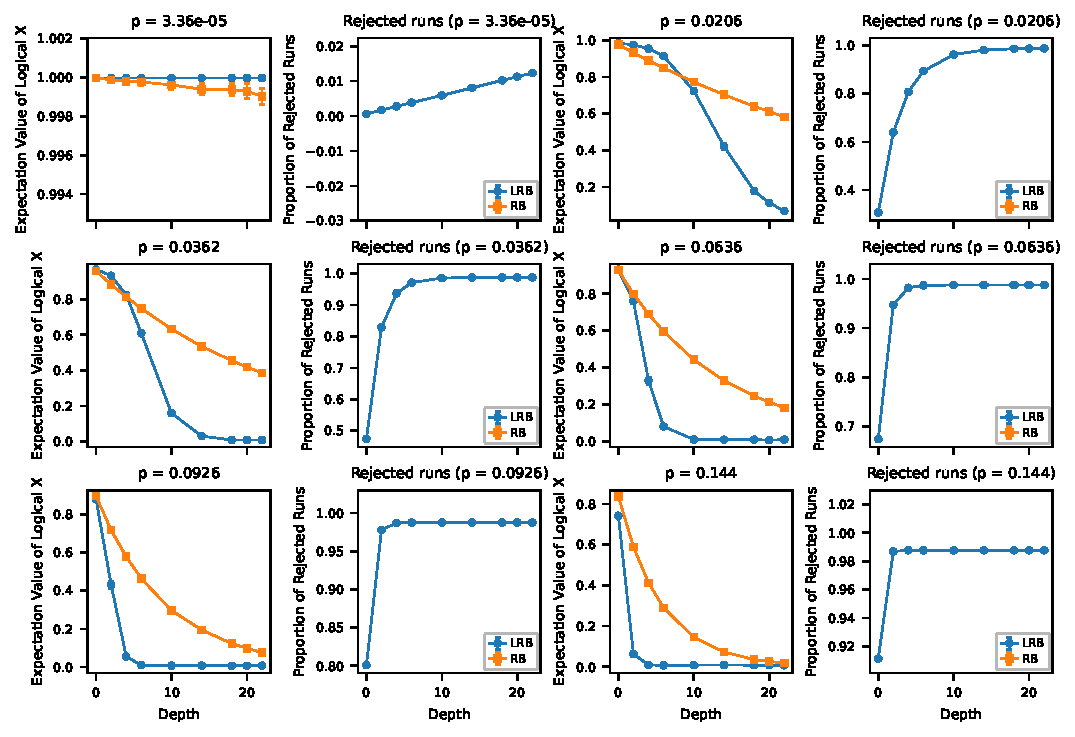
\includegraphics[width=0.95\textwidth]{
    figures/const-0-Summary-Graph-NoFit.pdf}
  \caption{Terminal post-selection. We pick out 6 $p$ values that display the non-Markovian evolution of the LRB-D traces. Columns 1 and 3: $\langle \bar{X}\rangle$ versus logical depth for
    LRB-D (blue) compared to a $\langle {X}\rangle$ versus physical RB baseline (orange). Columns 2 and 4: fraction of rejected shots versus depth. The LRB-D traces
    are visibly non-exponential, consistent with depth-dependent
    mixing among many decay modes when stabilizer filtering is applied
    only at the end of the sequence.}
  \label{fig:sim_terminal_nofit}
\end{figure}

\subsubsection{Uniform-interval post-selection: interpolating between
Markovian and non-Markovian regimes}
We next perform uniform-interval post-selection,
where stabilizers are checked every $k$ logical Cliffords and the run
is rejected as soon as a non-trivial syndrome is detected. This
introduces an adjustable reset timescale for the syndrome degrees
of freedom. All fitting in this subsection is confined to these
interval-check runs. The accepted-shot survival curves are fit to the
decay model of Eq.~\eqref{eq:fseq} with the offset fixed to $B = 0$,
since a fully depolarized logical qutrit yields a vanishing $\bar{X}$
expectation, and fidelities are extracted through Eq.~\eqref{eq:fbar}.

\paragraph{Near-Markovian limit ($k=1$).}
For $k=1$, the code-space projector is effectively applied after
every logical gate. Empirically, this recovers decay curves that are
well-approximated by a single exponential, as seen in
\autoref{fig:sim_unif1_fit}. Conceptually, frequent projection
suppresses the buildup of syndrome memory and collapses the dynamics
toward the minimal two-eigenvalue structure familiar from single-qutrit
RB (a trivial mode and a Pauli mode), in sharp contrast to the
high-multiplicity structure discussed in \autoref{sub:irreps}.

\begin{figure}[H]
  \centering
  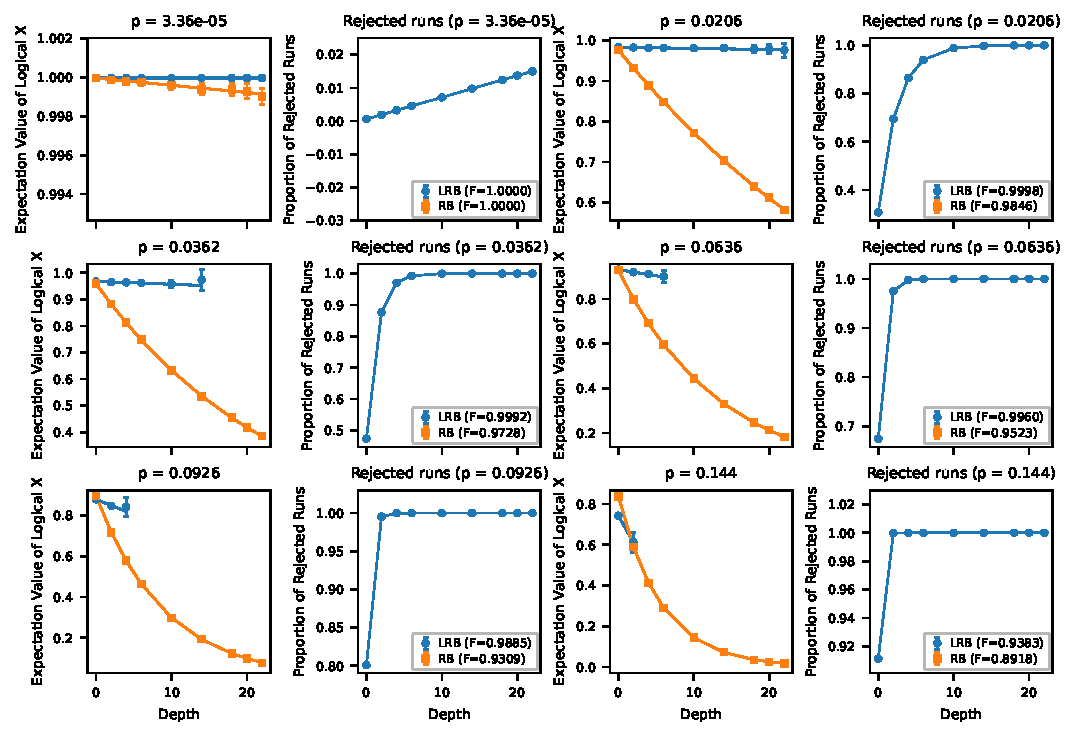
\includegraphics[width=0.95\textwidth]{
    figures/unif-1-Summary-Graph-Fit.pdf}
  \caption{Uniform interval $k=1$.
    Frequent stabilizer filtering largely restores a single-exponential
    decay model for LRB-D, at the expense of rapidly
    increasing rejection with $p$ and $m$. The \texttt{F} in the legend represents the average (logical) gate fidelity, and we notice that we get a significant improvement in fidelity due to the encoding.}
  \label{fig:sim_unif1_fit}
\end{figure}

\paragraph{Intermediate intervals ($k=2,3,4$).}
Observing \autoref{fig:sim_unif2_fit}, \autoref{fig:sim_unif3_fit}, and \autoref{fig:sim_unif4_fit}, for $k=2,3,4$, we still obtain usable single-exponential
approximations across much of the sweep, but
small deviations become more apparent as $k$ increases. Interpreted
through \autoref{sub:irreps}, these deviations reflect the gradual
reintroduction of additional decay modes associated with the many
copies of $V_{triv}$ and $V_{pauli}$ that become accessible within
each $k$-gate window. In other words, uniform-interval post-selection
interpolates between the two-mode RB-like limit ($k=1$) and the
strongly multi-mode terminal limit.

\begin{figure}[H]
  \centering
  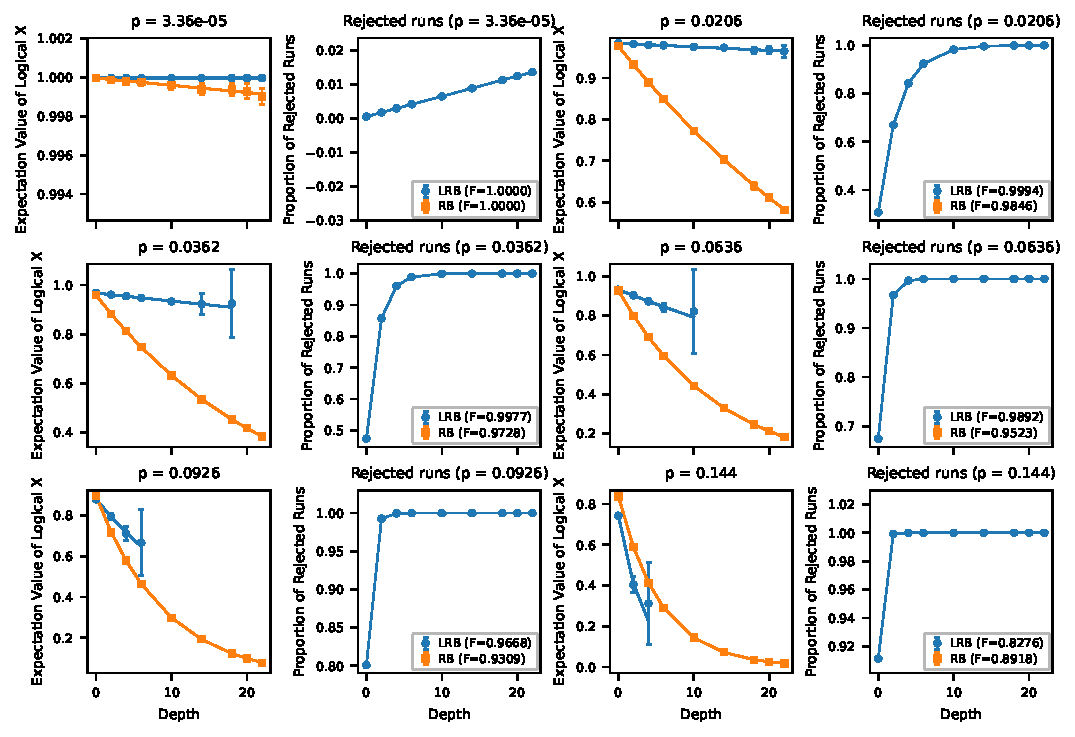
\includegraphics[width=0.95\textwidth]{
    figures/unif-2-Summary-Graph-Fit.pdf}
  \caption{Uniform interval $k=2$.
    Single-exponential fits remain a good approximation, but the
    extracted decay begins to show mild contamination from additional
    modes permitted between checks.}
  \label{fig:sim_unif2_fit}
\end{figure}

\begin{figure}[H]
  \centering
  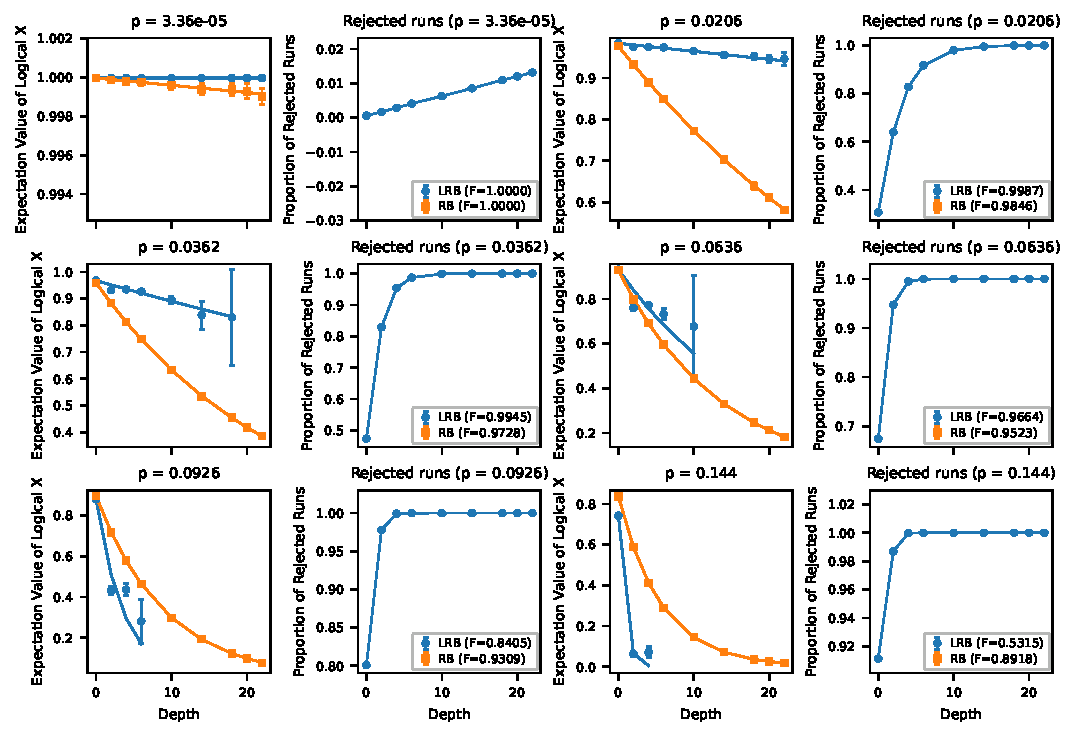
\includegraphics[width=0.95\textwidth]{
    figures/unif-3-Summary-Graph-Fit.pdf}
  \caption{Uniform interval $k=3$.
    Increasing the time between projections further increases the
    influence of syndrome-sector dynamics and amplifies departures
    from a pure single-mode decay.}
  \label{fig:sim_unif3_fit}
\end{figure}

\begin{figure}[H]
  \centering
  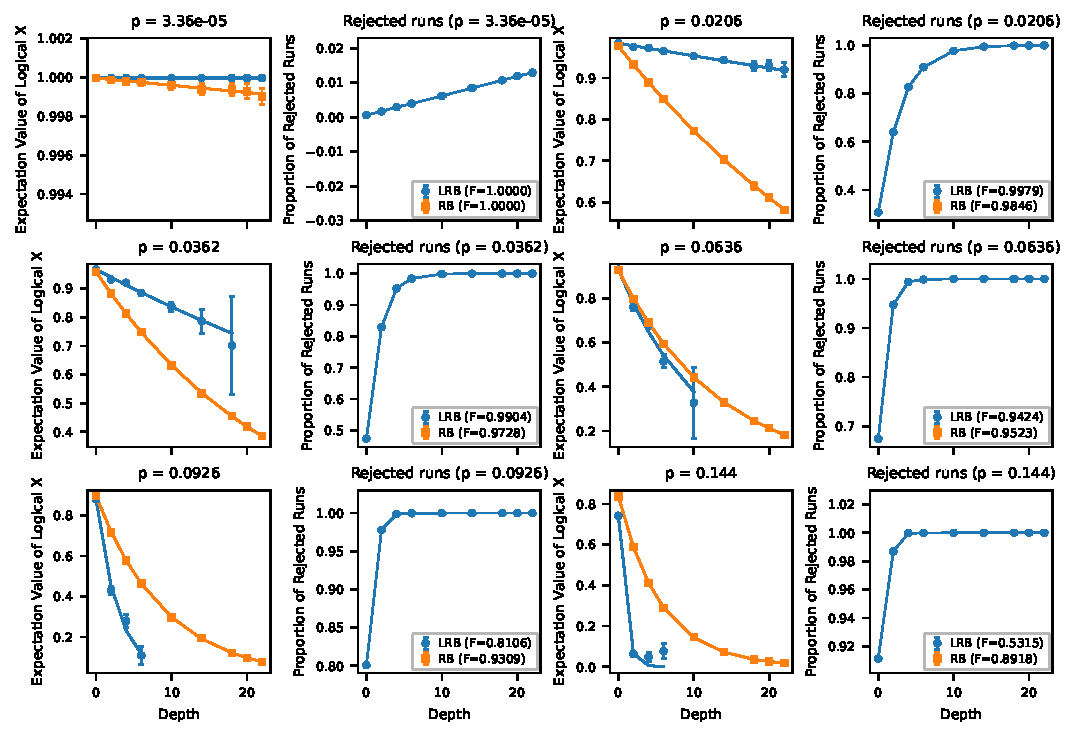
\includegraphics[width=0.95\textwidth]{
    figures/unif-4-Summary-Graph-Fit.pdf}
  \caption{Uniform interval $k=4$.
    A practical compromise regime: yields improve relative to $k=1$
    while remaining close enough to exponential behavior to extract an
    effective decay rate in much of the sweep.}
  \label{fig:sim_unif4_fit}
\end{figure}

\paragraph{Extreme intervals: re-emergent non-Markovianity.}
At large check intervals, the LRB-D curves become visibly more
irregular and less amenable to a single-exponential description.
\autoref{fig:sim_unif22_fit} shows an extreme example
(\texttt{$k=11$}), where the fitted curve captures only an average
trend while the data exhibit clear multi-timescale structure,
reflecting increased mixing among the many irrep-associated eigenmodes
between stabilizer projections. More generally, when $k$
becomes large, it no longer makes sense to interpret the LRB-D trace
through a single Markovian exponential decay model. The post-selected
(acceptance-conditioned) dynamics within the code manifold can mix
multiple irrep-associated decay modes \emph{in a depth-dependent way}
over each interval, so enforcing a fit to Eq.~\eqref{eq:fseq} becomes
a coarse phenomenological summary rather than a meaningful logical
fidelity estimator. In our folded-code sweeps, we observe that beyond about
$k=4$ the curves become strongly non-exponential across a substantial
portion of the parameter range, with visibly increasing non-Markovian
structure. For this reason, we focus our quantitative fitting and
pseudo-threshold extraction on $k=1$ through $k=4$,
using larger $k$ primarily to illustrate the non-Markovian crossover.

\begin{figure}[H]
  \centering
  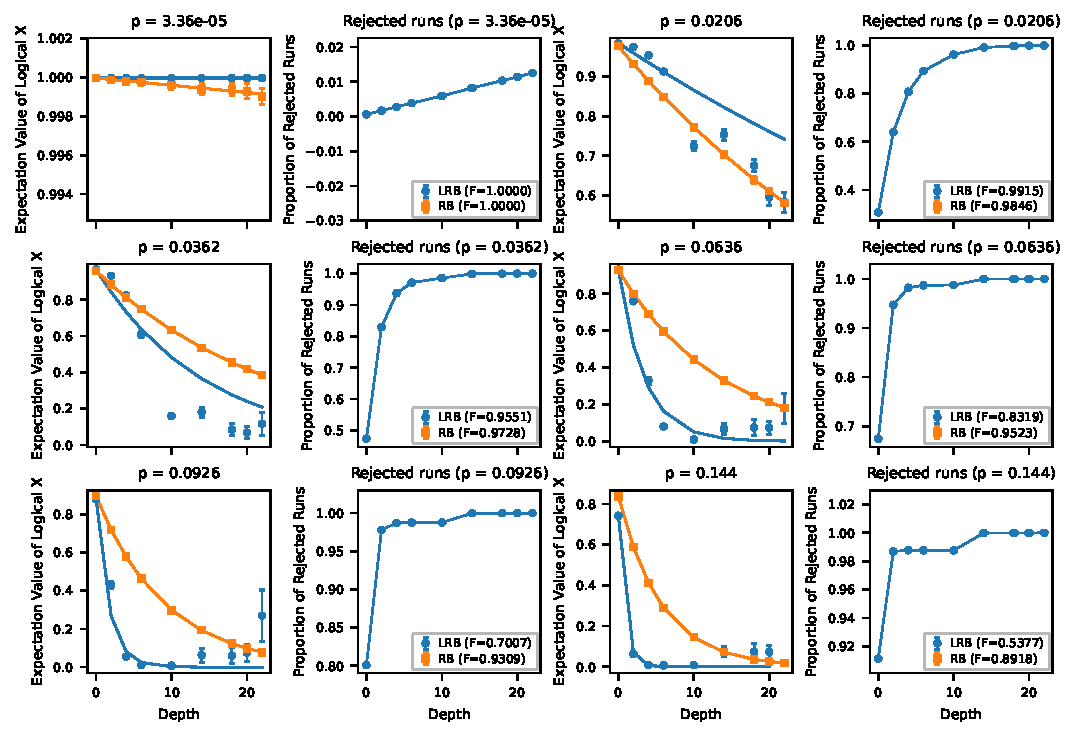
\includegraphics[width=0.95\textwidth]{
    figures/unif-11-Summary-Graph-Fit.pdf}
  \caption{Extreme uniform interval $k=11$.
    With rare stabilizer filtering throughout a logical Clifford sequence, the syndrome bath has time to
    develop substantial memory, and non-Markovian features re-emerge
    even under uniform interval post-selection.}
  \label{fig:sim_unif22_fit}
\end{figure}

\subsubsection{Pseudo-threshold analysis and the cost of post-selection}
In \autoref{fig:pseudo_threshold_panels}, we restrict the
pseudo-threshold analysis to $k=1$ through $k=4$.
To quantify when LRB-D provides an advantage over an unencoded
physical baseline, we compare the extracted error rates from (i)
LRB-D under uniform $k$-interval post-selection and (ii) standard
single-qutrit RB under the same physical noise parameter $p$. For each
$k$, we define a \emph{pseudo-threshold} $p^\star(k)$ as the value of
$p$ where the fitted LRB-D error rate intersects the fitted RB error
rate. Below $p^\star(k)$, the post-selected logical protocol exhibits
lower error than the physical reference. Above $p^\star(k)$, the
benefits of encoding are outweighed by the accumulated error paths
and the severe acceptance loss.

\begin{figure}[H]
  \centering
  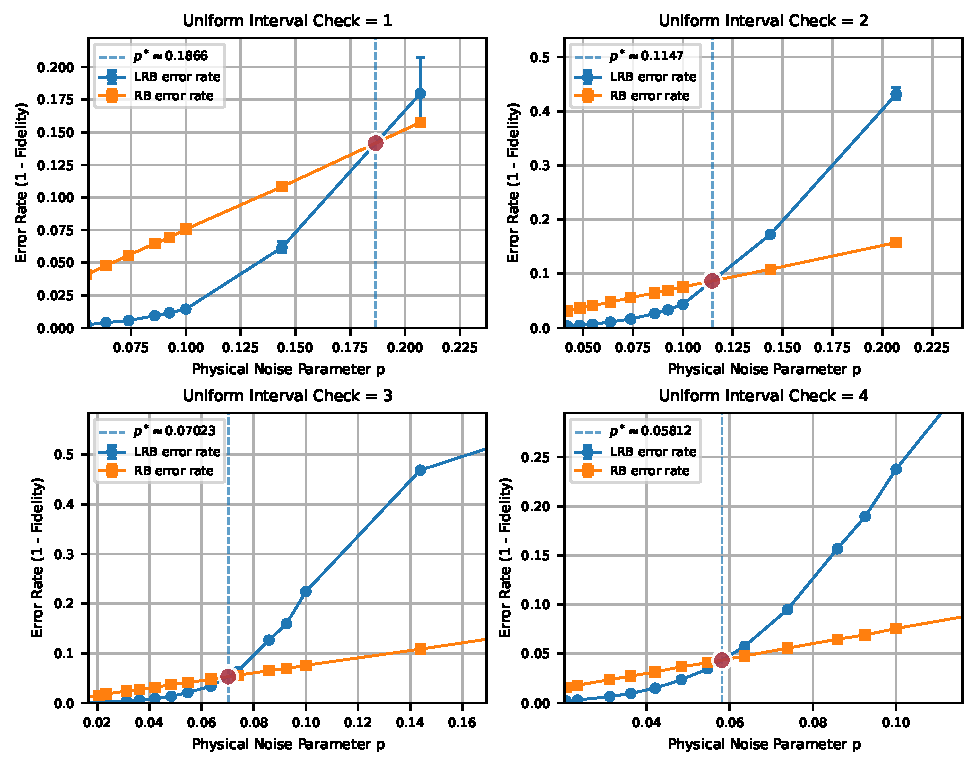
\includegraphics[width=\textwidth]{figures/unif-threshold-error-vs-p-paper-grid.pdf}
  \caption{Pseudo-threshold construction for uniform-interval post-selection.
    We plot fitted RB and LRB-D error rates versus $p$ for uniform check intervals
    $k=1,2,3,4$ and define $p^\star(k)$ by their intersection. As we get more liberal with our intervals, we observe that the pseudo-threshold starts to drop. However, the tradeoff is that we have more shot acceptances at each error parameter $p$.}
  \label{fig:pseudo_threshold_panels}
\end{figure}

For the folded $[[5,1,2]]_3$ patch, we find
$p^\star(1)\approx 0.186611 \pm 0.012320$,
$p^\star(2)\approx 0.114679 \pm 0.000768$,
$p^\star(3)\approx 0.070231 \pm 0.000258$,
and $p^\star(4)\approx 0.058116 \pm 0.000202$.
\autoref{fig:pseudo_threshold_trend} summarizes the decline
of $p^\star(k)$ with increasing $k$, quantifying the intuitive and
irrep-consistent statement that allowing longer syndrome sector
correlation times degrades the effective logical protection.

\begin{figure}[H]
  \centering
  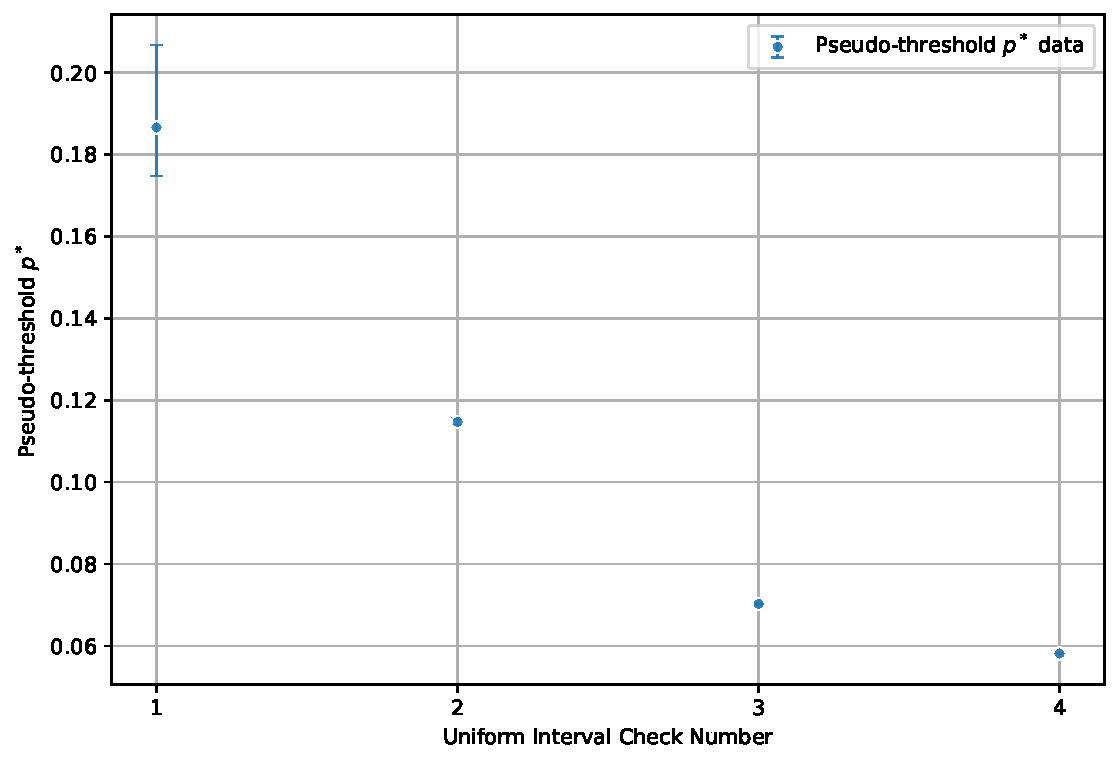
\includegraphics[width=0.65\textwidth]{
    figures/unif-1-to-4-pseudo-threshold-vs-interval-check-fit.pdf}
  \caption{Pseudo-threshold versus check interval. The
    pseudo-threshold decreases rapidly as stabilizer checks become less
    frequent, reflecting increased multi-mode contamination and
    longer-lived syndrome memory between projections to the codespace.}
  \label{fig:pseudo_threshold_trend}
\end{figure}

Post-selection is essential here because $[[5,1,2]]_3$ is an error-\emph{detection} code: it allows us to benchmark a small early-FTQC patch
without committing to an ambiguous decoder and violating Knill-Laflamme's error correction conditions. It also provides a tunable
knob ($k$) that cleanly exposes the crossover from RB-like (two-mode)
exponential decay to multi-mode, non-Markovian behavior described in
\autoref{sub:irreps}. 

The principal drawback is sampling overhead: as
seen in the rejection panels of \autoref{fig:sim_unif1_fit}--
\autoref{fig:sim_unif22_fit}, the accepted fraction can collapse
quickly with $p$ and depth, requiring very large shot counts to
maintain statistical power. Moreover, because LRB-D reports a
\emph{conditional} logical performance (conditioned on no detected
error), it does not directly represent the unconditional reliability
of a long computation. Instead, it characterizes the quality of the
logical dynamics within the detected code manifold and how strongly
they are perturbed by excursions into syndrome sectors.

\subsection{LRB-D under SI1000 Noise}
\label{sub:si1000_results}

We next benchmark the folded $[[5,1,2]]_3$ patch under the qutrit SI1000 noise model of \autoref{subsub:si1000_model}. The protocol is unchanged from \autoref{sub:simulation_results}. Each stabilizer generator is measured with its own ancilla, so the simulated system consists of nine qutrits, five data and four ancillas. We sweep 15 raw noise strengths $p$ from $0$ to $0.05$, corresponding to normalized strengths $\lambda = 5p$ from $0$ to $0.25$, with logical depths up to $m=22$ and $10^6$ shots per depth spread over 30 independent random Clifford sequences. These runs are sampled through the compiled detector error model backend of \autoref{sec:sdim-dem}, which is what makes this shot count affordable across the full grid of check schedules.

The physical reference is single-qutrit RB with the depolarizing channel $\mathcal{E}_{\mathcal{D}}(p_{RB})$ applied after every Clifford, simulated at $p_{RB} = \lambda$ on the matching grid with $10^4$ shots per depth. Since $\lambda$ is the flip rate on each ancilla readout, the worst single location in the encoded circuit, the comparison asks whether an encoded qutrit whose worst location fails at rate $\lambda$ can outperform a bare qutrit that suffers that same rate at every gate.

\subsubsection{Terminal post-selection}
In the terminal regime no stabilizer checks are inserted during the sequence, and the accept or reject decision is made only once, from the terminal $X$-basis data readout by evaluating the two $X$-type stabilizers on the recorded outcomes. \autoref{fig:si1000_terminal} shows the resulting traces. The LRB-D curves again fail to follow a single exponential, with a flat shoulder at small depth followed by a faster decay, which is the same multi-mode syndrome memory discussed in \autoref{sub:irreps}. For this reason we extract no fit parameters in the terminal regime. Compared to the depolarizing results of \autoref{fig:sim_terminal_nofit}, however, the departure is visibly milder, and the encoded traces now sit above the matched physical baseline across the entire sweep. The reason is the SI1000 rate hierarchy. Between checks the logical Cliffords only pick up single-qutrit noise at rate $p/10 = \lambda/50$ and entangling noise at rate $\lambda/5$, so at a fixed value of the noise coordinate the encoded sequence accumulates far less error than the depolarizing model injects, while the physical baseline is held at the full rate $\lambda$ per gate.

\begin{figure}[H]
  \centering
  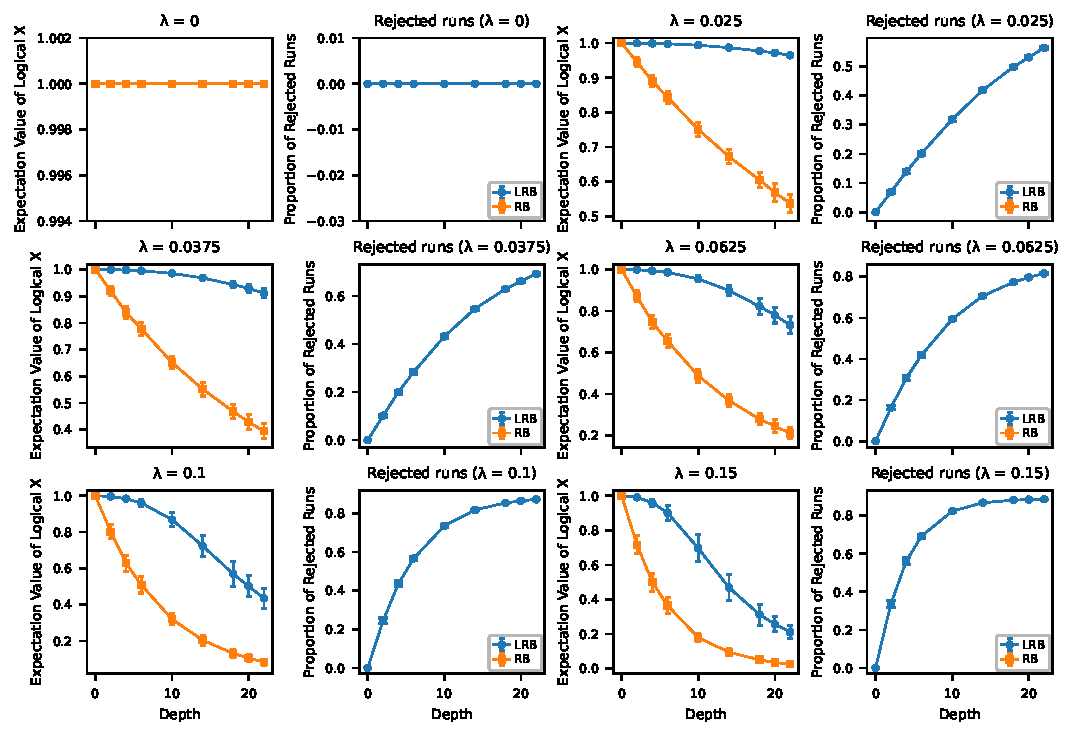
\includegraphics[width=0.95\textwidth]{
    figures/si1000-const-0-Summary-Graph-NoFit.pdf}
  \caption{Terminal post-selection under qutrit SI1000 noise. We pick out six representative values of $\lambda$ up to $0.15$. Columns 1 and 3: $\langle \bar{X}\rangle$ versus logical depth for LRB-D (blue) compared to the $\langle X \rangle$ physical RB baseline at $p_{RB}=\lambda$ (orange). Columns 2 and 4: fraction of rejected shots versus depth. The LRB-D traces remain non-exponential, but the deviation is milder than in the depolarizing model and the encoded qutrit retains an advantage over the matched physical baseline throughout.}
  \label{fig:si1000_terminal}
\end{figure}

\subsubsection{Uniform-interval post-selection}
We then apply uniform-interval post-selection, checking all four stabilizers every $k$ logical Cliffords and rejecting a shot as soon as any check returns a non-trivial outcome. All fitting in this section is confined to these interval-check runs. For each $k$ we fit the accepted-shot survival curves to the decay model of Eq.~\eqref{eq:fseq} with the offset fixed to $B = 0$, following the convention of \autoref{sub:simulation_results}. The physical RB baseline is fit with the same zero-offset model, and fidelities are extracted through Eq.~\eqref{eq:fbar}.

\paragraph{Near-Markovian limit ($k=1$).}
As in the depolarizing case, checking after every logical Clifford collapses the dynamics back toward a two-mode structure, and the decay curves in \autoref{fig:si1000_unif1_fit} are well described by a single exponential. The encoded advantage below threshold is substantial. At $\lambda = 0.025$ we extract an average logical gate fidelity of $\bar{F} = 0.9993$ against a physical $\bar{F} = 0.9814$, and at $\lambda = 0.1$ we obtain $0.9710$ against $0.9288$. By $\lambda = 0.15$ the two are statistically indistinguishable, at $0.8980$ against $0.8965$, which is consistent with the pseudo-threshold extracted below. The cost of this regime is that every check layer now carries its own noise. Each of the four ancilla readouts flips at rate $5p = \lambda$, so a sizable fraction of shots is rejected by the very first check layer even at depth zero, and the rejected fraction saturates toward one within a few logical gates at moderate $\lambda$.

\begin{figure}[H]
  \centering
  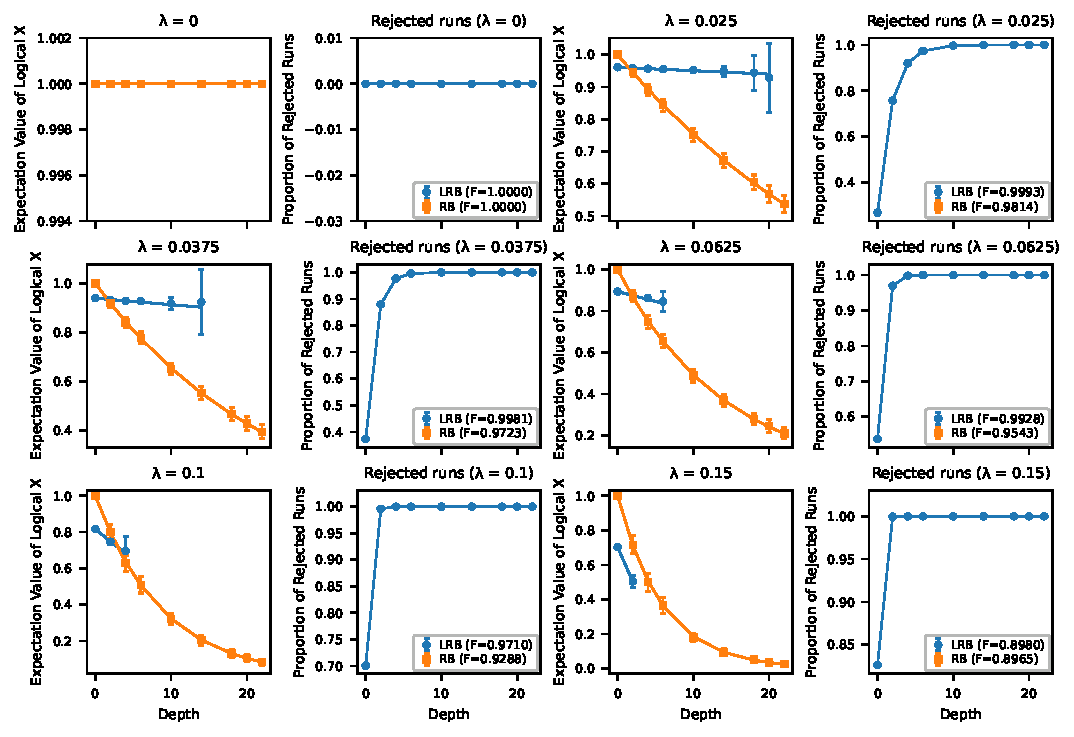
\includegraphics[width=0.95\textwidth]{
    figures/si1000-unif-1-Summary-Graph-Fit.pdf}
  \caption{Uniform interval $k=1$ under qutrit SI1000 noise. Frequent stabilizer filtering restores a single-exponential decay for LRB-D, and the fitted logical fidelities \texttt{F} show a clear improvement over the matched physical baseline below the pseudo-threshold. The noisy check layers make the acceptance cost front-loaded, with substantial rejection already at depth zero.}
  \label{fig:si1000_unif1_fit}
\end{figure}

\paragraph{Intermediate intervals ($k=2,3,4$).}
Spacing the checks out, shown in \autoref{fig:si1000_unif2_fit}, \autoref{fig:si1000_unif3_fit}, and \autoref{fig:si1000_unif4_fit}, trades acceptance for fit quality in the same way as in the depolarizing model. Single-exponential fits remain usable across most of the sweep, with small deviations growing as $k$ increases and more decay modes become accessible between projections. The deviations grow more slowly with $k$ than they did under depolarizing noise, which again reflects how little error the SI1000 model injects between check layers at fixed $\lambda$. As before, we restrict quantitative fitting and threshold extraction to $k \le 4$, and beyond this range the traces develop the same strongly non-exponential features seen in the depolarizing sweeps.

\begin{figure}[H]
  \centering
  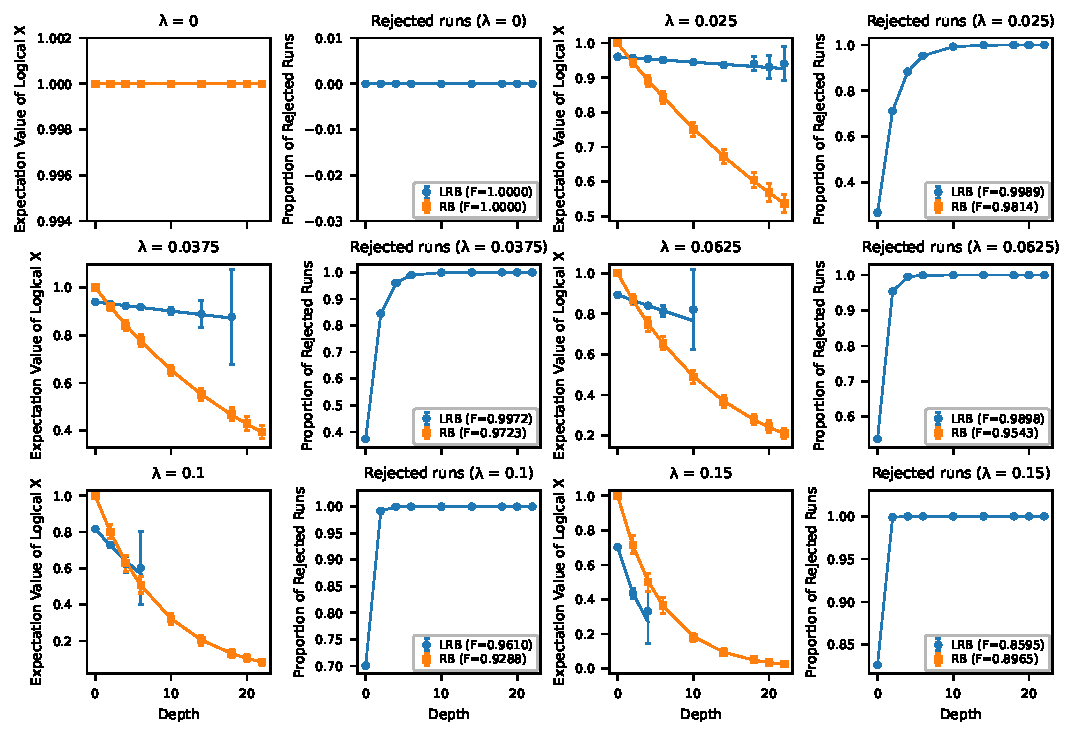
\includegraphics[width=0.95\textwidth]{
    figures/si1000-unif-2-Summary-Graph-Fit.pdf}
  \caption{Uniform interval $k=2$ under qutrit SI1000 noise. Halving the check frequency improves acceptance while the fits remain close to single-exponential.}
  \label{fig:si1000_unif2_fit}
\end{figure}

\begin{figure}[H]
  \centering
  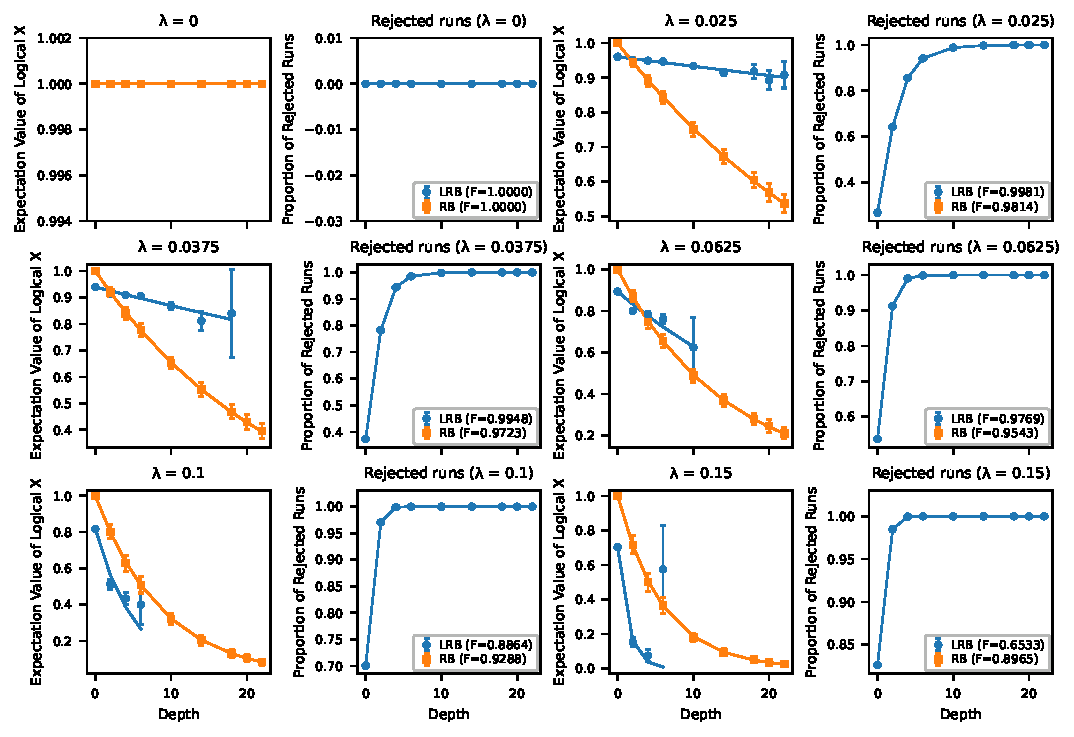
\includegraphics[width=0.95\textwidth]{
    figures/si1000-unif-3-Summary-Graph-Fit.pdf}
  \caption{Uniform interval $k=3$ under qutrit SI1000 noise. Mild multi-mode contamination becomes visible in the extracted decays as the interval grows.}
  \label{fig:si1000_unif3_fit}
\end{figure}

\begin{figure}[H]
  \centering
  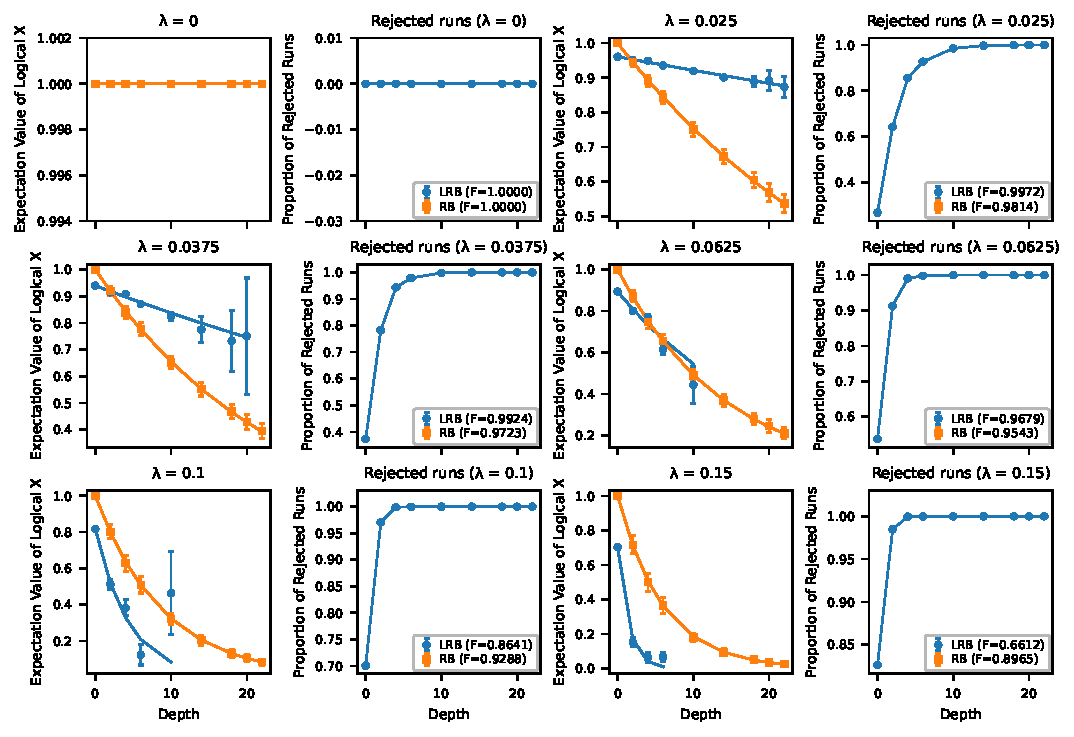
\includegraphics[width=0.95\textwidth]{
    figures/si1000-unif-4-Summary-Graph-Fit.pdf}
  \caption{Uniform interval $k=4$ under qutrit SI1000 noise. As in the depolarizing model this is a practical compromise, with better yields than $k=1$ and decays that are still close enough to exponential to fit.}
  \label{fig:si1000_unif4_fit}
\end{figure}

\subsubsection{Pseudo-thresholds}
\autoref{fig:si1000_threshold_panels} repeats the pseudo-threshold construction of \autoref{sub:simulation_results} on the SI1000 interval-check data, plotting the LRB-D error rate fitted for each uniform check interval at coordinate $\lambda$ against the fitted physical RB error rate at $p_{RB} = \lambda$ and defining $\lambda^\star(k)$ by their intersection. Error bars on the fitted rates are 68\% bootstrap intervals over 500 resamples, and threshold uncertainties use 1000 bootstrap resamples. For the folded patch we find
$\lambda^\star(1) \approx 0.150569 \pm 0.002474$,
$\lambda^\star(2) \approx 0.123274 \pm 0.001336$,
$\lambda^\star(3) \approx 0.079668 \pm 0.000573$,
and $\lambda^\star(4) \approx 0.072530 \pm 0.000871$,
where the quoted uncertainties are bootstrap standard deviations. The bootstrap intervals are mildly asymmetric, for example the 68\% interval for $\lambda^\star(1)$ is $[0.1473, 0.1520]$.

\begin{figure}[H]
  \centering
  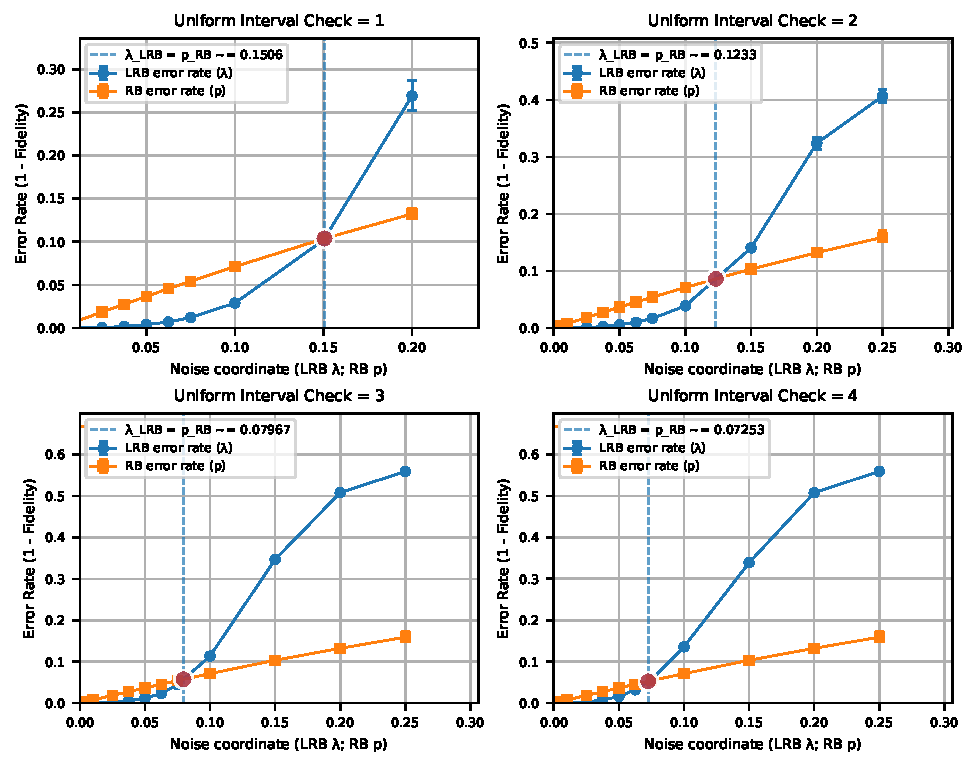
\includegraphics[width=\textwidth]{figures/si1000-unif-threshold-error-vs-p-paper-grid.pdf}
  \caption{Pseudo-threshold construction under qutrit SI1000 noise for uniform check intervals $k=1,2,3,4$. Fitted LRB-D error rates at coordinate $\lambda$ are compared against fitted physical RB error rates at $p_{RB}=\lambda$, and $\lambda^\star(k)$ is defined by their intersection. The RB baseline is linear in $p_{RB}$ as expected for the depolarizing channel, while the LRB-D error rates rise steeply once the check layers and entangling gates dominate.}
  \label{fig:si1000_threshold_panels}
\end{figure}

The trend with $k$, summarized in \autoref{fig:si1000_threshold_trend}, is instructive when placed next to the depolarizing results. At $k=1$ the SI1000 pseudo-threshold sits below the depolarizing value of $p^\star(1) \approx 0.187$, which we attribute to the check layers themselves. Under SI1000 the ancilla readouts are the noisiest locations in the circuit, so checking after every logical gate maximizes exposure to exactly the operations the model penalizes most. For $k \ge 2$ the ordering reverses, with the SI1000 thresholds at $0.123$, $0.080$, and $0.073$ sitting above their depolarizing counterparts of $0.115$, $0.070$, and $0.058$. With so little noise accumulating between checks, spacing the projections out costs less than it does under depolarizing noise, and the decline of $\lambda^\star(k)$ with $k$ is correspondingly shallower. From $k=1$ to $k=4$ the threshold falls by a factor of about $2.1$ under SI1000 compared to about $3.2$ under depolarizing noise.

\begin{figure}[H]
  \centering
  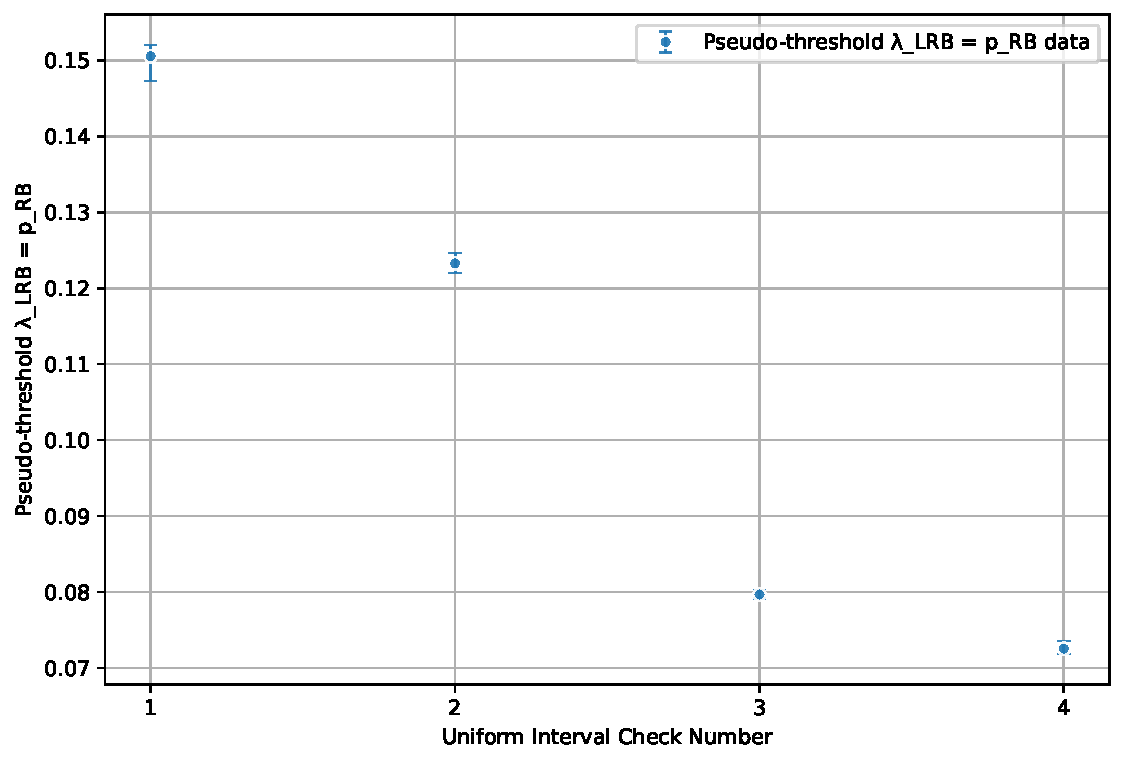
\includegraphics[width=0.65\textwidth]{
    figures/si1000-unif-1-to-4-pseudo-threshold-vs-interval-check-fit.pdf}
  \caption{Pseudo-threshold versus check interval under qutrit SI1000 noise. The threshold decreases as checks become less frequent, but more slowly than in the depolarizing model, since the SI1000 rate hierarchy concentrates the noise in the check layers rather than in the logical gates between them.}
  \label{fig:si1000_threshold_trend}
\end{figure}

The acceptance overhead deserves the same caveat as before. Because the check layers are the dominant noise locations, uniform-interval post-selection under SI1000 rejects aggressively, and past moderate $\lambda$ the accepted fraction at $k=1$ collapses within a few logical gates. The $10^6$ shots per depth point provided by the DEM backend are what keep the accepted-shot statistics usable deep into the sweep. The conditional interpretation of LRB-D discussed at the end of \autoref{sub:simulation_results} carries over unchanged.


\subsection{IQM QPU}


\appendix

\section{Representation Theory}\label{sec:rep-theory}

\subsection{Group Modules and Irreducible Representations}

The aim of this section if to serve as a review of the basics of representation theory.
This will not be an exhaustive review by any means.
For a more thorough mathematical treatment of the representation of finite groups we direct the reader to \cite{sagan2001symmetric}.

Let $G$ denote a finite group. We will denote the identity element of $G$ by $e$ to avoid confusion. 
A $G$-module is a finite dimensional vector space $V$ equipped with a group action $\cdot : G \times V \to V$ satisfying 
\begin{enumerate}
    \item \textbf{(Identity)} For all vectors $\ket{v} \in V$, the equality $e \cdot \ket{v} = \ket{v}$ is satisfied.
    \item \textbf{(Linearity)} For all linear combinations $\alpha \ket{v} + \beta \ket{w}$ and all group elements $g \in G$, the equality $g \cdot (\alpha \ket{v}+\beta\ket{b}) = \alpha (g\cdot \ket{v}) + \beta (g \cdot \ket{w})$ is satisfied.
    \item \textbf{(Compatability)} For all group elements $g,h \in G$ and vectors $\ket{v} \in V$, the equality $(gh) \cdot \ket{v} = g\cdot (h \cdot \ket{v})$ is satisfied.
\end{enumerate}
The linearity axiom implies the existence of a map $\pi: G \to \mathrm{End}(V)$ mapping the group element $g$ to the linear endomorphism $\ket{v} \mapsto g\cdot \ket{v}$. 
The identity and compatibility axioms imply that $\pi$ is actually a group homomorphism. 

\begin{lemma}
    We call a group homomorphism $\pi : G \to \mathrm{End}(V)$ a representation of $G$. If $\pi: G \to \mathrm{End}(V)$ is a representation, then $V$ is a $G$-module under 
    \begin{align}
        g \cdot \ket{v} = \pi(G)\ket{v}.
    \end{align}
    Moreover, if $V$ is a $G$-module, then the map $\pi(g)(\ket{v}) = g\cdot \ket{v}$ is a representation of $G$.
\end{lemma}
In light of this result, it is somewhat standard to conflate representation of $G$ and $G$-modules. 
As with all linear maps, representations are typically described by how each element of $G$ acts on each basis vector of $V$.
% Alternatively, one can describe a representation by first describing how the group $G$ acts on some set $X$ and then extending the action to the free vector space $\mathbb{C}[X]$ by linearity.

Sometimes, a representation can be reduced to a direct sum of smaller representations in the sense that 
\begin{align}
    \pi(g) = \pi_0(g) \oplus \pi_1(g) \oplus \dots \oplus \pi_k(g)
\end{align}
for each $\pi_i$ a representation.
In this case, we write $\pi = \pi_0 \oplus \dots \oplus \pi_k$.
This corresponds to a decomposition of $G$-modules $V = V_0 \oplus \dots \oplus V_k$ where each $V_i$ is a $G$-module.
If no such decomposition exists, then we call the representation (or $G$-module) irreducible.
Irreducible representations are typically referred to by the abbreviation ``irrep''.

\begin{theorem}[Maschke's Theorem \cite{sagan2001symmetric} Theorem 1.5.3] \label{thm:maschkes-theorem}
    Every representation $\pi : G \to \mathrm{End}(V)$ decomposes into a direct sum
    \begin{align}
        \pi \cong m_0 \pi_0 \oplus m_1 \pi_1 \oplus \dots \oplus m_k \pi_k
    \end{align}
    where $\pi_i$ and $\pi_j$ are distinct irreducible representations of $G$. Here $m_i \pi_i \cong \bigoplus_{j=0}^{m_i - 1} \pi_i$.

    Similarly, if $V$ is a finite dimensional $G$-module, then 
    \begin{align}
        V = m_0 V_0 \oplus \dots \oplus m_k V_k
    \end{align}
    where $V_i$ and $V_j$ are distinct irreducible $G$-modules.
\end{theorem}
Maschke's theorem requires two important caveats. 
Firstly, we must be working over an algebraically closed field. 
Secondly, it must be possible to average over the group, so an analog of Maschke's theorem holds for compact Lie groups.

\subsubsection{Schur's Lemma}

Suppose that $V$ is a $G$-module. 
We let $\mathrm{End}_G(V)$ denote all of the elements $T \in \mathrm{End}_G(V)$ such that for all $g \in G$
\begin{align}
    T \pi(g) = \pi(g)T.
\end{align}
Elements of $T$ are said to be invariant under the action of $G$ or $G$-linear.
This condition ends up being rather stringent.

\begin{lemma}[Schur's Lemma \cite{sagan2001symmetric} Theorem 1.6.5]\label{lem:schurs-lemma}
    Let $V$ and $W$ be $G$-modules and let $\pi_V$ and $\pi_W$ be the associated representations.
    We define $\mathrm{Hom}_G(V, W)$ by $T \in \mathrm{Hom}_G(V, W)$ if for all $g \in G$
    \begin{align}
        T \pi_V(g) = \pi_W(g) T.
    \end{align}
    If $V$ and $W$ are irreducible, then exactly one of the following holds.
    \begin{enumerate}
        \item The $G$-modules $V$ and $W$ are not isomorphic and $\mathrm{Hom}_G(V,W) = 0$.
        \item The $G$-modules $V$ and $W$ are isomorphic and $\mathrm{Hom}_G(V,W) \cong \mathbb{C}$ in the sense that $\mathrm{End}_G(V) = \{ \lambda I_V \mid \lambda \in \mathbb{C} \}$.
    \end{enumerate}
\end{lemma}

\begin{cor}[\cite{sagan2001symmetric} Theorem 1.7.9]
    Let $V$ be a $G$-module with such that
    \begin{align}
        V = m_0 V_0 \oplus \dots \oplus m_k V_k
    \end{align}
    with $V_i$ and $V_j$ distinct irreducible modules.
    Let $d_i$ be the dimension of $V_i$.
    Then the following hold.
    \begin{enumerate}
        \item The dimension of $V$ is given by $\mathrm{dim}(V) = m_0 d_0 + \dots + m_k d_k$.
        \item \label{item:artin-wedderburn} The endomorphism algebra of $V$ is isomorphic to the direct sum
        \begin{align}
            \mathrm{End}_G(V) \cong \bigoplus_{i = 0}^k \mathrm{End}(\mathbb{C}^{m_i}).
        \end{align}
        \item The endomorphism algebra $\mathrm{End}_G(V)$ has dimension $m_0^2 + m_1^2 + \dots + m_k^2$.
    \end{enumerate}
\end{cor}

\begin{proof}
    We will only include a proof of \Cref{item:artin-wedderburn} as it is the most important.
    From the decomposition of $V$, we get the equality
    \begin{align}
        \mathrm{End}_G(V) \cong \bigoplus_{i,j = 0}^k \mathrm{Hom}_G(m_iV_i,m_jV_j).
    \end{align}
    The elements of $\mathrm{Hom}_G(m_i V_i, m_j V_j)$ can be thought of as $m_i \times m_j$ matrices whose entries are in $\mathrm{Hom}_G(V_i, V_j)$. 
    However, if $i \neq j$, the by Schur's lemma we know that $\mathrm{Hom}_G(V_i, V_j)$ only contains the zero map. 
    Thus, all of the terms in the direct sum for $i \neq j$ are zero and can be ignored. 
    When $i = j$, the elements of $\mathrm{Hom}_G(V_i,V_i) = \mathrm{End}_G(V_i)$ are all multiples of the identity map. 
    So, the elements $g_i \in \mathrm{End}_G(m_iV_i)$ can be written in the form
    \begin{align}
        g_i = M_i \otimes I_{V_i},
    \end{align}
    where $M_i \in \mathrm{End}(\mathbb{C}^{m_i})$ is an $m_i \times m_i$ matrix with complex entries. 
    % Moreover, any such matrix $M_i$ defines an element $g_i = M_i \otimes I_{V_i} \in \mathrm{End}_G(m_i V_i)$.
    A routine argument shows $\mathrm{End}_G(m_iV_i)$ is isomorphic to the matrix algebra $\mathrm{End}(\mathbb{C}^{m_i})$ under the map $g_i \mapsto M_i$.
    Finally, we conclude that $\mathrm{End}_G(V) \cong \bigoplus_{i = 0}^k \mathrm{End}_G(m_i V_i)$ and hence
    \begin{align}
        \mathrm{End}_G(V) \cong \bigoplus_{i=0}^k \mathrm{End}(\mathbb{C}^{m_i}).
    \end{align}
\end{proof}

Concretely, Schur's lemma and its corollary impose a relatively stringent structure on the elements of $\mathrm{End}_G(V)$. 
For our purposes the most important property is that if $T \in \mathrm{End}_G(V)$ and $\ket{v} \in m_i V_i$ is supported entirely in copies of the $V_i$ module, then $T\ket{v} \in m_i V_i$ is also supported entirely in copies of $V_i$. 
The following result guarantees that the twirled error channel that we aim to study is invariant under the action of the Clifford group.

\begin{lemma}[Twirling] \label{lem:twirling}
    Suppose $V$ is a finite dimensional $G$-module with associated representation for $G$ finite. Given any $T \in \mathrm{End}(V)$ (notably $T$ need not be $G$-linear), the twirled map
    \begin{align}
        T_G = \frac{1}{|G|} \sum_{g \in G} \pi(g)^{-1} T \pi(g)
    \end{align}
    is an element of $\mathrm{End}_G(V)$.
\end{lemma}

\begin{proof}
    Fix $g \in G$. Conjugating $T_G$ by $\pi(g)$ yields 
    \begin{align}
        \pi(g)^{-1} T_G \pi(g) = \frac{1}{|G|} \sum_{h \in G} \pi(g)^{-1} \pi(h)^{-1} T \pi(h) \pi(g) = \frac{1}{|G|} \sum_{h \in G} \pi(hg)^{-1} T \pi(hg).
    \end{align}
    Since the right coset $Gg$ is equal to $G$, we can reindex the sum to obtain 
    \begin{align}
        \pi(g)^{-1} T_G \pi(g) = \frac{1}{|G|} \sum_{h \in G} \pi(hg)^{-1} T \pi(hg) = \frac{1}{|G|} \sum_{h \in G} \pi(h)^{-1} T \pi(h) = T_G.
    \end{align}
    We conclude that $\pi(g)^{-1} T_G \pi(g) = T_G$ and hence $T_G \pi(g) = \pi(g) T_G$.
\end{proof}

\subsection{Character Theory}

\Cref{item:artin-wedderburn} and \Cref{lem:twirling} show us that in order to fully understand a twirled channel, it is necessary to understand how many copies of each irreducible representation are present in a given representation.
Luckily, if the irreps are understood, then there is an efficient algorithm for computing how many copies of that irrep occur in the decomposition.
This technique comes from a subject called character theory.

\subsubsection{Characters and Conjugacy Classes}

If $\pi : G \to \mathrm{End}(V)$ is a representation, then the character $\chi_\pi : G \to \mathbb{C}$ of $\pi$ is defined by 
\begin{align}
    \chi_\pi(g) = \Tr \pi(g).
\end{align}
By the cyclic property of the trace, characters satisfy the property $\chi_\pi(h g h^{-1}) = \chi_\pi(g)$.
Because of this, characters are constant on the conjugacy classes.
Such a function is called a class function.
Evidently, the space of class functions has dimension equal to the number of conjugacy classes of $G$.
Moreover, the space is equipped with a natural inner product 
\begin{align}
    \langle \chi, \tau \rangle = \frac{1}{|G|} \sum_{g \in G} \chi(g)^* \tau(g).
\end{align}
The following lemma is among the most important results in character theory.

\begin{lemma}[Character Orthogonality \cite{sagan2001symmetric} Theorem 1.9.3] \label{lem:character-orthogonality}
    If $\pi_1$ and $\pi_2$ are irreducible representations of the finite group $G$, then 
    \begin{align}
        \langle \chi_{\pi_1}, \chi_{\pi_2}\rangle = \begin{cases}
            1 & \pi_1 \cong \pi_2, \\
            0 & \text{otherwise}.
        \end{cases}
    \end{align}
\end{lemma}

\begin{cor}[\cite{sagan2001symmetric} Corollary 1.9.4] \label{cor:character-relations}
    Let $\pi : G \to \mathrm{End}(V)$ be a representation and $\pi = m_0 \pi_1 \oplus \dots \oplus m_k \pi_k$ be the decomposition of the representation $\pi$ into irreps. The following hold.
    \begin{enumerate}
        \item The character $\chi_{\pi}$ can be written as $\chi_{\pi} = m_0 \chi_{\pi_0} + m_1 \chi_{\pi_1} + \dots + m_k \chi_{\pi_k}$.
        \item \label{item:irrep-mult-test} The inner product $\langle \chi_{\pi}, \chi_{\pi_i}\rangle = m_i$ for all $0 \leq i \leq k$.
        \item The inner product $\langle \chi_{\pi}, \chi_{\pi} \rangle = m_0^2 + \dots + m_k^2$. In particular this is always an integer.
        \item The representation $\pi$ is irreducible if and only if $\langle \chi_{\pi}, \chi_{\pi} \rangle = 1$.
        \item If $\tau$ is another representation of $G$, then $\pi$ and $\tau$ are isomorphic if and only if $\chi_{\pi}(g) = \chi_{\tau}(g)$ for all $g \in G$.
    \end{enumerate}
\end{cor}

\Cref{lem:character-orthogonality} and \Cref{cor:character-relations} show us two remarkable facts.
Firstly, the irrep characters are orthonormal and thus linearly independent.
From this we can conclude that the irrep characters form a basis for the space of class functions and, in particular, that there must be exactly as many irreps as there are conjugacy classes of $G$.
Secondly, \Cref{item:irrep-mult-test} gives us an efficient method of determining how many copies of a given irrep are present in an arbitrary representation of $G$.

\section{The \texttt{sdim} Simulator and Detector Error Model Sampling}
\label{sec:sdim-dem}

This appendix describes the simulation machinery behind the numerical results, namely the \texttt{sdim} qudit stabilizer simulator and the compact $q$-ary detector error model (DEM) backend used for the SI1000 sweep.

\subsection{Qudit stabilizer simulation}

\texttt{sdim} \cite{sdim} is a tableau-based stabilizer simulator for prime-dimensional qudits. It generalizes the binary tableau formalism of \cite{Aaronson2004} to arithmetic over $\mathbb{Z}_q$, representing stabilizer generators as Weyl operators $\omega^c X^{\mathbf{a}} Z^{\mathbf{b}}$ with exponent vectors $\mathbf{a}, \mathbf{b} \in \mathbb{Z}_q^n$ \cite{Gottesman1999,Hostens2005}. Clifford gates act on the tableau by linear updates of these exponent vectors, and computational or Fourier-basis measurements are handled by the qudit analog of the usual stabilizer measurement rules. All circuits in this work use $q=3$.

Noise is included through parameterized Pauli channels, inserted as explicit noise operations in the circuit. The single-qutrit operation carries a channel tag and a probability. The depolarizing tag applies a uniformly random non-identity $X^a Z^b$ with the stated probability, the shift tag applies a uniformly random non-identity power of $X$, and the phase tag applies a uniformly random non-identity power of $Z$, matching the channels defined in \autoref{sub:noise_models}. The two-qutrit operation applies a uniformly random non-identity two-qutrit Pauli, or samples from an explicitly supplied distribution over all $81$ two-qutrit Paulis.

Rather than rerunning the tableau algorithm shot by shot, \texttt{sdim} samples in the Pauli frame picture. A single noiseless reference shot is simulated with the full tableau algorithm. For every additional shot, only a Pauli frame, one pair of exponents $(a_i, b_i)$ per qutrit, is propagated through the Clifford circuit. Noise operations update the frame stochastically, and each measurement returns the reference outcome shifted by the frame content on the measured qutrit modulo three. This separates the polynomially expensive stabilizer computation, done once, from the cheap per-shot frame propagation.

\subsection{Detectors and logical observables}

A detector is a linear combination of measurement records, $D = \sum_i c_i m_i \bmod 3$ with integer coefficients $c_i$, chosen so that $D$ takes a fixed known value on every noiseless execution of the circuit. A logical observable is the same kind of expression, except that its value carries logical information instead of being fixed. This is the qudit generalization of the detector formalism introduced by Stim for qubit circuits \cite{Gidney2021Stim}, with sums modulo two replaced by sums modulo three and with coefficients in $\{\pm 1\}$ to account for daggered stabilizer components.

Our LRB-D circuits declare one detector per stabilizer check, labeled by the check round and the ancilla wire. Since every ancilla is freshly reset before its syndrome extraction block, the noiseless value of each ancilla readout is zero, and the detector is simply that readout. The post-selection rule of the protocol, keeping only shots in which every check returns the trivial syndrome, is then exactly the statement that every detector vanished. The terminal logical observable is $m_0 + m_3 \bmod 3$ evaluated on the final $X$-basis readouts of qutrits $q_0$ and $q_3$, matching $\bar{X} = X_0 \otimes X_3$. In the terminal-only protocol, where all five data qutrits are read out directly in the $X$ basis, the two $X$-type stabilizers are declared as detectors with the coefficient patterns $m_0 + m_1 - m_2$ and $m_3 - m_1 - m_4$, mirroring $G_3$ and $G_4$.

\subsection{Compiling the detector error model}

A detector error model is a list of the independent fault locations in the circuit, each with its firing probability and its effect on every detector and logical observable. The key structural fact is linearity. A fault $X^a Z^b$ inserted at some location propagates through the remaining Clifford circuit to a final Pauli whose exponents depend linearly on $(a,b)$, and detector values are themselves linear in the measurement outcomes modulo three. Consequently the shift that a fault induces on any detector is
\begin{equation}
    \Delta D = a\, r_X + b\, r_Z \bmod 3,
\end{equation}
where $r_X$ and $r_Z$ are the responses to the unit faults $X$ and $Z$ at that location. A two-qutrit fault location behaves the same way with four unit responses. It therefore suffices to probe each noise location with two unit faults for a single-qutrit channel or four for a two-qutrit channel.

Compilation proceeds directly through the frame simulator. For every noise location and every unit component, we run the frame simulation with exactly that one unit fault inserted and all other noise disabled, and record the difference of every detector and logical observable against a fault-free baseline, modulo three. The probing runs are batched, and the result is a sparse table that maps each location and unit component to the list of detectors and logical observables it shifts, together with the coefficient of the shift. Locations whose channel probability is zero are dropped. The compiled model is cached per circuit, so the probing cost is paid once for each annotated circuit regardless of how many shots are later sampled.

\subsection{Sampling and exactness}

Sampling the compiled model is elementary. For each shot, every active location fires independently with its probability. When a location fires, the fault exponents are drawn according to its channel, a uniformly random non-zero pair $(a,b)$ for depolarizing noise, a non-zero $a$ alone for the shift channel, a non-zero $b$ alone for the phase channel, and a uniformly random non-zero four-tuple for the two-qutrit channel. The corresponding responses, scaled by the drawn exponents, are accumulated into the detector and logical event arrays modulo three. A shot is accepted precisely when every accumulated detector value is zero, and the logical outcome is the reference outcome shifted by the accumulated logical response.

Because our noise models consist entirely of Pauli channels acting inside a Clifford circuit, and because faults compose additively in the frame picture, this procedure reproduces exactly the joint distribution of detector and logical events that direct frame simulation would produce. Nothing is approximated. What changes is the cost profile. After the one-time compilation, the per-shot work is proportional to the number of active noise locations and the sparsity of their responses, and is independent of the stabilizer computation itself. This is what made the SI1000 production grid of \autoref{sub:si1000_results} affordable across its 45 stabilizer check schedules.


\section{Generating the Single-Qutrit Clifford Group}
\label{sec:clifford-gen}

Both the physical RB and the logical LRB-D protocols sample uniformly from the single-qutrit Clifford group, so we need an explicit catalog of its elements, a realization of each element as a circuit, and a fast way to look up inverses for the recovery gate. This appendix records how that catalog is constructed.

Modulo global phases, the single-qutrit Clifford group $\mathcal{C}_3$ contains $216$ elements. It factors into the qutrit Pauli group and the quotient $\mathcal{C}_3 / \mathcal{P}_3$, which is isomorphic to the symplectic group $Sp(2,\mathbb{Z}_3) = SL(2,\mathbb{Z}_3)$ of order $24$ \cite{Appleby2005,Hostens2005}. Counting phase-free Pauli representatives $X^a Z^b$ with $a,b \in \mathbb{Z}_3$ gives $9$ elements, and $9 \times 24 = 216$. We exploit this factorization and build the group in two stages, first the $24$ coset representatives and then their products with the $9$ Pauli monomials.

\paragraph{Coset representatives from a Cayley graph.}
The quotient $\mathcal{C}_3/\mathcal{P}_3$ is generated by the images of $H$ and $S$. We represent each generator by its conjugation action on the eight non-identity Pauli classes $\{X, Z, XZ, X^2, Z^2, X^2Z, Z^2X, X^2Z^2\}$, which realizes the quotient faithfully as a permutation group on eight symbols. We then perform a breadth-first traversal of the Cayley graph of this group. Starting from the identity, every known element is multiplied on the right by each generator, and the first time a new element is produced we record its label as the label of its parent extended by the corresponding generator symbol. Because the traversal is breadth-first, each of the $24$ elements receives a minimal-length word in $H$ and $S$, and the traversal terminates once all $24$ are found. Repeated symbols are then compressed into power notation, so for instance $SSHS$ becomes $S^2HS$. The graph explored by this traversal is shown in \autoref{fig:cayley-c3modp3}, with every node carrying the canonical word that the traversal assigned to it.

\begin{figure}[H]
  \centering
  \resizebox{0.92\textwidth}{!}{%
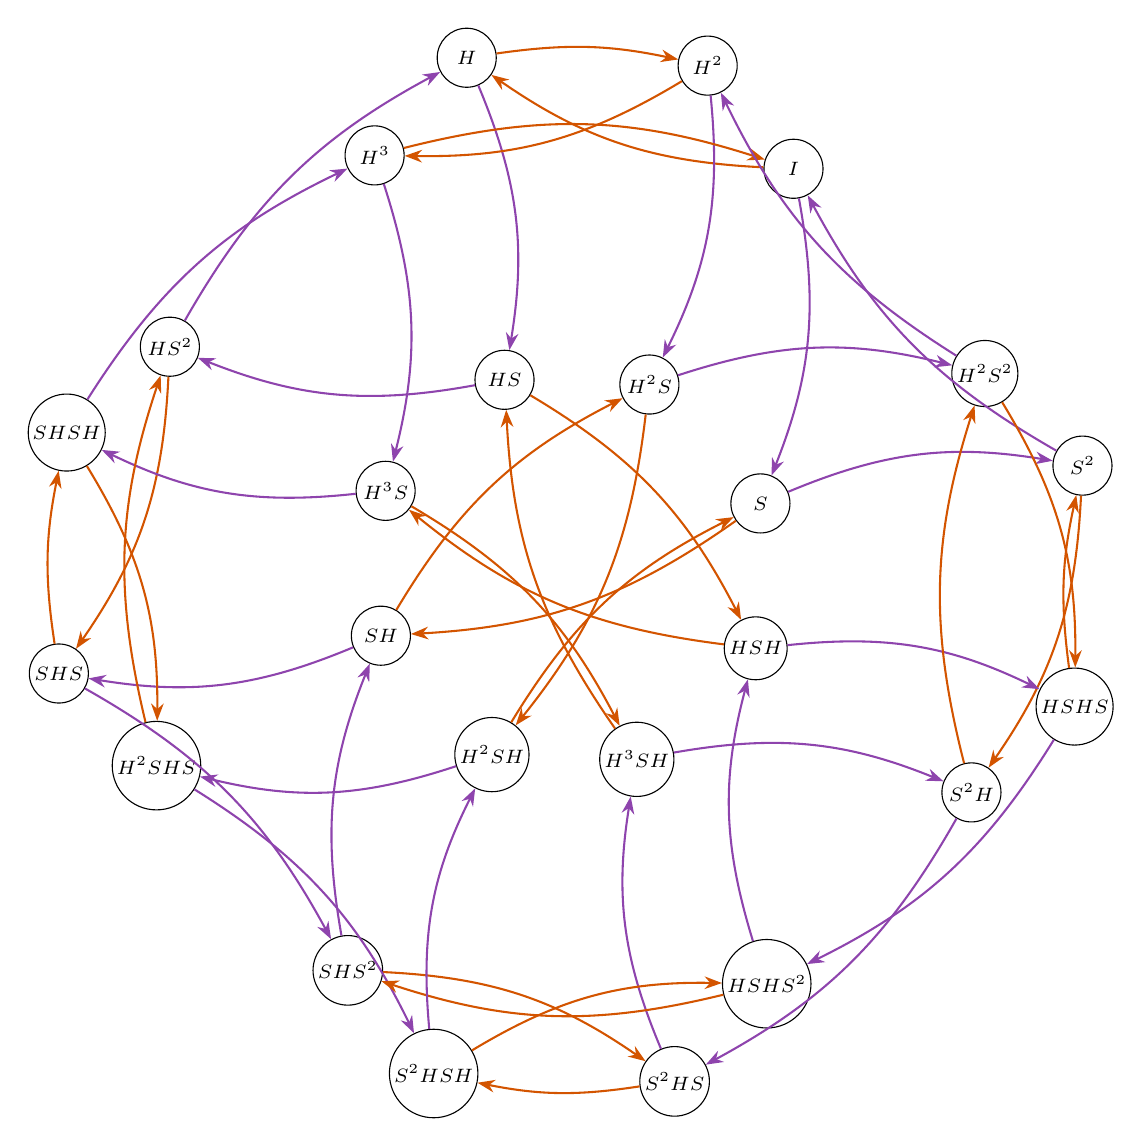
\begin{tikzpicture}[>={Stealth[length=2.2mm,width=1.6mm]},
  cnode/.style={circle,draw=black,fill=white,inner sep=1.1pt,minimum size=7.5mm,font=\scriptsize},
  Hedge/.style={->,HCol,line width=0.75pt},
  Sedge/.style={->,SwapCol,line width=0.75pt}]
  \node[cnode] (n0) at (2.83,5.09) {$I$};
  \node[cnode] (n1) at (-1.32,6.5) {$H$};
  \node[cnode] (n2) at (2.41,0.84) {$S$};
  \node[cnode] (n3) at (1.74,6.4) {$H^2$};
  \node[cnode] (n4) at (-0.84,2.41) {$HS$};
  \node[cnode] (n5) at (-2.41,-0.84) {$SH$};
  \node[cnode] (n6) at (6.5,1.32) {$S^2$};
  \node[cnode] (n7) at (-2.49,5.26) {$H^3$};
  \node[cnode] (n8) at (1.0,2.35) {$H^2S$};
  \node[cnode] (n9) at (2.35,-1.0) {$HSH$};
  \node[cnode] (n10) at (-5.09,2.83) {$HS^2$};
  \node[cnode] (n11) at (-6.5,-1.32) {$SHS$};
  \node[cnode] (n12) at (5.09,-2.83) {$S^2H$};
  \node[cnode] (n13) at (-2.35,1.0) {$H^3S$};
  \node[cnode] (n14) at (-1.0,-2.35) {$H^2SH$};
  \node[cnode] (n15) at (5.26,2.49) {$H^2S^2$};
  \node[cnode] (n16) at (6.4,-1.74) {$HSHS$};
  \node[cnode] (n17) at (-6.4,1.74) {$SHSH$};
  \node[cnode] (n18) at (-2.83,-5.09) {$SHS^2$};
  \node[cnode] (n19) at (1.32,-6.5) {$S^2HS$};
  \node[cnode] (n20) at (0.84,-2.41) {$H^3SH$};
  \node[cnode] (n21) at (-5.26,-2.49) {$H^2SHS$};
  \node[cnode] (n22) at (2.49,-5.26) {$HSHS^2$};
  \node[cnode] (n23) at (-1.74,-6.4) {$S^2HSH$};
  \draw[Hedge] (n0) to[bend left=16] (n1);
  \draw[Sedge] (n0) to[bend left=16] (n2);
  \draw[Hedge] (n1) to[bend left=10] (n3);
  \draw[Sedge] (n1) to[bend left=16] (n4);
  \draw[Hedge] (n2) to[bend left=16] (n5);
  \draw[Sedge] (n2) to[bend left=16] (n6);
  \draw[Hedge] (n3) to[bend left=16] (n7);
  \draw[Sedge] (n3) to[bend left=16] (n8);
  \draw[Hedge] (n4) to[bend left=16] (n9);
  \draw[Sedge] (n4) to[bend left=16] (n10);
  \draw[Hedge] (n5) to[bend left=16] (n8);
  \draw[Sedge] (n5) to[bend left=16] (n11);
  \draw[Hedge] (n6) to[bend left=16] (n12);
  \draw[Sedge] (n6) to[bend left=16] (n0);
  \draw[Hedge] (n7) to[bend left=16] (n0);
  \draw[Sedge] (n7) to[bend left=16] (n13);
  \draw[Hedge] (n8) to[bend left=16] (n14);
  \draw[Sedge] (n8) to[bend left=16] (n15);
  \draw[Hedge] (n9) to[bend left=16] (n13);
  \draw[Sedge] (n9) to[bend left=16] (n16);
  \draw[Hedge] (n10) to[bend left=16] (n11);
  \draw[Sedge] (n10) to[bend left=16] (n1);
  \draw[Hedge] (n11) to[bend left=10] (n17);
  \draw[Sedge] (n11) to[bend left=16] (n18);
  \draw[Hedge] (n12) to[bend left=16] (n15);
  \draw[Sedge] (n12) to[bend left=16] (n19);
  \draw[Hedge] (n13) to[bend left=16] (n20);
  \draw[Sedge] (n13) to[bend left=16] (n17);
  \draw[Hedge] (n14) to[bend left=16] (n2);
  \draw[Sedge] (n14) to[bend left=16] (n21);
  \draw[Hedge] (n15) to[bend left=16] (n16);
  \draw[Sedge] (n15) to[bend left=16] (n3);
  \draw[Hedge] (n16) to[bend left=10] (n6);
  \draw[Sedge] (n16) to[bend left=16] (n22);
  \draw[Hedge] (n17) to[bend left=16] (n21);
  \draw[Sedge] (n17) to[bend left=16] (n7);
  \draw[Hedge] (n18) to[bend left=16] (n19);
  \draw[Sedge] (n18) to[bend left=16] (n5);
  \draw[Hedge] (n19) to[bend left=10] (n23);
  \draw[Sedge] (n19) to[bend left=16] (n20);
  \draw[Hedge] (n20) to[bend left=16] (n4);
  \draw[Sedge] (n20) to[bend left=16] (n12);
  \draw[Hedge] (n21) to[bend left=16] (n10);
  \draw[Sedge] (n21) to[bend left=16] (n23);
  \draw[Hedge] (n22) to[bend left=16] (n18);
  \draw[Sedge] (n22) to[bend left=16] (n9);
  \draw[Hedge] (n23) to[bend left=16] (n22);
  \draw[Sedge] (n23) to[bend left=16] (n14);
\end{tikzpicture}
  }
  \caption{Cayley graph of the quotient $\mathcal{C}_3/\mathcal{P}_3 \cong SL(2,\mathbb{Z}_3)$ generated by the traversal described in the text. Each of the $24$ nodes is one coset representative, labeled by the power-compressed word assigned to it when the breadth-first traversal first reached it. Orange arrows denote right multiplication by $H$ and purple arrows denote right multiplication by $S$. The $S$ arrows close into eight directed $3$-cycles and the $H$ arrows close into six directed $4$-cycles, reflecting the orders of the two generators, and every element is reachable from the identity $I$ within five generator applications.}
  \label{fig:cayley-c3modp3}
\end{figure}


\paragraph{Full expressions.}
The full catalog is the set of products $P \cdot C$, where $P$ ranges over the nine Pauli monomials and $C$ over the $24$ coset words. After normalizing the identity cases and removing duplicates, this yields exactly $216$ canonical expression strings, such as $X^2Z^2S^2HSH$. These strings are the sampling alphabet for every benchmark in this work. For the physical RB baseline, each string is parsed into its symbol and power tokens and the corresponding primitive gates are multiplied out into a single unencoded qutrit gate.

\paragraph{Logical realization.}
For the encoded protocol, each primitive symbol in an expression is replaced by its transversal logical implementation on the folded $[[5,1,2]]_3$ patch. The logical $\bar{H}$ and $\bar{S}$ are the constant-depth circuits of \autoref{fig: logical H} and \autoref{fig: logical S}, and the logical Paulis act as $\bar{X} = X_0 \otimes X_3$ and $\bar{Z} = Z_0 \otimes Z_2$. Since the expression strings are written as operator products, with the leftmost factor acting last, the substitution walks each string in reverse so that the resulting circuit applies the factors in the correct temporal order. Finally, runs of consecutive single-qutrit gates on the same physical wire are merged into single composite gates between the entangling operations. This keeps the depth of each logical Clifford close to the depth of its generating set rather than growing with the word length.

\paragraph{Inverses.}
The recovery gate $\bar{C}_{inv} = (\prod_{i=1}^m \bar{C}_i)^{-1}$ is never synthesized at run time. Instead, the group multiplication over the catalog is precomputed, and each catalog element is stored together with the expression of its inverse. Constructing the inverse of a sampled sequence then reduces to a table lookup followed by the same logical realization as any other group element.

The construction is implemented once in Cirq for the unencoded and encoded gate objects, and the resulting expression catalog together with its per-symbol gate decompositions is what the \texttt{sdim} simulation pipeline of \autoref{sub:sim_framework} consumes.


Both Marxer et al.~\cite{Marxer2023} and Luo et al.~\cite{Luo2023}
implement entangling gates by applying a baseband flux pulse to a
tunable transmon coupler. The pulse changes the interaction between
two data transmons and thereby controls their relative phases.
The relevant quantity is the \emph{conditional phase}: the phase of
a joint state after subtracting the phases attributable to the
individual systems. If a diagonal operation maps
$\ket{ij}\rightarrow e^{i\theta_{ij}}\ket{ij}$, the conditional
phase is
\begin{equation}
    \phi_{ij}
    = \theta_{ij}-\theta_{i0}-\theta_{0j}+\theta_{00}.
    \label{eq:conditional-phase}
\end{equation}
This quantity is invariant under local diagonal corrections and
therefore characterizes the entangling part of the operation.
A two-qubit CZ gate requires $\phi_{11}=\pi$, whereas the
generalized two-qutrit CZ gate requires a prescribed pattern of
four conditional phases.

\paragraph{Two-qubit CZ through a coherent excursion.}

In Marxer's implementation, the qubits are biased near the
$\ket{11}\leftrightarrow\ket{20}$ resonance. The coupler index is
omitted in this notation. Using the approximate transmon spectrum,
\begin{equation}
    \frac{E_{11}}{\hbar}\simeq\omega_1+\omega_2,
    \qquad
    \frac{E_{20}}{\hbar}\simeq2\omega_1+\alpha_1,
\end{equation}
where $\omega_1$ and $\omega_2$ are the qubit transition angular
frequencies and $\alpha_1<0$ is the first transmon's anharmonicity.
The corresponding detuning is
\begin{equation}
    \delta
    = \frac{E_{20}-E_{11}}{\hbar}
    \simeq\omega_1-\omega_2+\alpha_1.
\end{equation}
A flux pulse applied to the coupler activates the effective
exchange interaction while the qubit biases remain fixed.
After subtracting the energy of $\ket{11}$, a minimal model for
the relevant subspace is
\begin{equation}
    \frac{H_{\mathrm{sub}}(t)}{\hbar}
    =
    \begin{pmatrix}
        0 & G(t)\\
        G(t) & \delta(t)
    \end{pmatrix}_{\{\ket{11},\ket{20}\}},
    \qquad
    G\simeq\sqrt{2}\,g_{\mathrm{eff}}.
    \label{eq:two-state-model}
\end{equation}
The factor $\sqrt{2}$ arises from the transmon ladder-operator
matrix element. Coupler dressing can modify both the effective
coupling and detuning during the pulse.

For constant coupling at exact resonance, $\delta=0$, the
evolution from $\ket{11}$ is
\begin{equation}
    \ket{\psi(t)}
    = \cos(Gt)\ket{11}-i\sin(Gt)\ket{20}.
\end{equation}
At $T=\pi/G$, the population completes a round trip and
\begin{equation}
    \ket{\psi(T)}=-\ket{11}.
\end{equation}
Although the population returns to its initial value, the
amplitude acquires a phase of $\pi$. This distinction between
population return and amplitude return provides the essential
intuition for the gate: the auxiliary state $\ket{20}$ allows a
cyclic excursion that changes the phase of the computational
state $\ket{11}$.

For a constant detuned pulse, the same model gives
\begin{equation}
    \Omega=\sqrt{\delta^2+4G^2},
    \qquad
    T=\frac{2\pi}{\Omega},
    \qquad
    \ket{11}\rightarrow
    e^{i(\pi-\delta T/2)}\ket{11},
    \label{eq:detuned-return}
\end{equation}
in the chosen frame. Thus, population return alone does not
guarantee the desired conditional phase. The experimental pulse
is shaped and slightly detuned, so
Eqs.~\eqref{eq:two-state-model}--\eqref{eq:detuned-return}
provide intuition rather than a complete model of the waveform.
The pulse must be calibrated to suppress final leakage and
satisfy
\begin{equation}
    \theta_{11}-\theta_{10}-\theta_{01}+\theta_{00}
    =\pi \pmod{2\pi}.
\end{equation}
After correcting the local phases, the resulting operation is
\begin{equation}
    U_{\mathrm{CZ}}=\operatorname{diag}(1,1,1,-1).
\end{equation}
Marxer et al.\ implement this evolution using a Slepian-shaped
coupler pulse, with a $22\,\mathrm{ns}$ interaction time and a
$33\,\mathrm{ns}$ duration including padding~\cite{Marxer2023}.

\paragraph{Two-qutrit controlled phase through energy shifts.}

Luo's experiment uses $\ket{0}$, $\ket{1}$, and $\ket{2}$ of each
data transmon as logical states. An effective description follows
the dressed computational states as the coupler frequency changes.
Let $E_{ij}$ denote their energies, with the ground-state coupler
index suppressed, and define
\begin{equation}
    \chi_{ij}(t)
    =
    \frac{
        E_{ij}(t)-E_{i0}(t)-E_{0j}(t)+E_{00}(t)
    }{\hbar},
    \qquad i,j\in\{1,2\}.
    \label{eq:cross-kerr}
\end{equation}
After removing local energy contributions, the effective
conditional Hamiltonian is
\begin{equation}
    \frac{H_{\mathrm{cond}}(t)}{\hbar}
    =
    \sum_{i,j=1}^{2}
    \chi_{ij}(t)\proj{ij}.
\end{equation}
Within this diagonal description, the accumulated phases are
\begin{equation}
    \phi_{ij}
    =-\int_0^T\chi_{ij}(t)\,dt,
    \label{eq:integrated-phase}
\end{equation}
where the sign follows the convention
$U=\mathcal{T}\exp[-(i/\hbar)\int_0^T H(t)\,dt]$.

The physical origin of these conditional shifts is multilevel
hybridization: a joint state's energy differs from the sum of
the corresponding individual energies. Changing the coupler
frequency controls this nonadditivity. Pulse amplitude therefore
controls the phase rates, while pulse duration controls the
accumulated angles. Equation~\eqref{eq:integrated-phase} includes
the contributions from both the ramps and the plateau.
Experimentally, the interaction shifts are calibrated using
conditional Ramsey measurements, which compare phase evolution
for different states of the other qutrit~\cite{Luo2023}.

The target operation is the generalized qutrit CZ,
\begin{equation}
    U_{\mathrm{CZ}_3}\ket{ij}
    =e^{i2\pi ij/3}\ket{ij},
    \qquad i,j\in\{0,1,2\}.
\end{equation}
Its four nontrivial conditional phases satisfy
\begin{equation}
    \begin{pmatrix}
        \phi_{11} & \phi_{12}\\
        \phi_{21} & \phi_{22}
    \end{pmatrix}
    =
    \begin{pmatrix}
        2\pi/3 & 4\pi/3\\
        4\pi/3 & 2\pi/3
    \end{pmatrix}
    \pmod{2\pi}.
    \label{eq:qutrit-target}
\end{equation}

Luo et al.\ construct this pattern using two identical coupler
flux pulses, separated and followed by simultaneous
$\ket{1}\leftrightarrow\ket{2}$ microwave swaps on both qutrits.
The time-ordered sequence is
\begin{equation}
    \text{flux pulse}
    \;\longrightarrow\;
    \text{swaps}
    \;\longrightarrow\;
    \text{flux pulse}
    \;\longrightarrow\;
    \text{swaps}.
\end{equation}
Suppose one flux pulse contributes conditional phases
$(a,b,c,d)$ to
$(\ket{11},\ket{12},\ket{21},\ket{22})$.
For ideal swaps, and up to local phase corrections, the complete
sequence contributes
\begin{equation}
    (\phi_{11},\phi_{12},\phi_{21},\phi_{22})
    =(a+d,\;b+c,\;b+c,\;a+d).
    \label{eq:phase-pairing}
\end{equation}
For example, an input $\ket{11}$ samples the $\ket{11}$
interaction shift during the first pulse and the $\ket{22}$
shift during the second. An input $\ket{22}$ samples the same
shifts in reverse order. The swaps therefore enforce equality
within each pair and reduce the calibration to two phase sums:
\begin{equation}
    a+d=\frac{2\pi}{3},
    \qquad
    b+c=\frac{4\pi}{3}
    \pmod{2\pi}.
\end{equation}

In the paper's qutrit--coupler--qutrit notation, the resulting
operation on the dressed computational manifold is
\begin{equation}
\begin{aligned}
    U_{\mathrm{Cphase}}
    ={}&
    e^{i2\pi/3}
    \left(\proj{101}+\proj{202}\right)\\
    &+
    e^{-i2\pi/3}
    \left(\proj{102}+\proj{201}\right)\\
    &+
    \sum_{\substack{
        i,j\in\{0,1,2\}\\
        i=0\ \mathrm{or}\ j=0
    }}
    \proj{i0j}.
\end{aligned}
\end{equation}
The middle zero denotes the ground-state coupler label.
The final sum specifies that states with either qutrit in
$\ket{0}$ acquire no conditional phase after local corrections.
The equality $e^{-i2\pi/3}=e^{i4\pi/3}$ makes the connection to
Eq.~\eqref{eq:qutrit-target} explicit~\cite{Luo2023}.


\bibliographystyle{unsrt}
\bibliography{references}

\end{document}
